\documentclass[a4paper]{article}

\usepackage[english]{babel}
\usepackage[utf8x]{inputenc}
\hyphenation{sig-nif-i-cant-ly}
\hyphenation{as-sess-ment}
\hyphenation{elec-tri-fi-ca-tion} 
\hyphenation{in-ter-pre-ta-tion}
\hyphenation{in-ter-pretabil-i-ty}
\hyphenation{con-struc-tion}
\hyphenation{char-ac-ter-izes}
\hyphenation{eco-nom-i-cal-ly}
\hyphenation{op-ti-miza-tion}
\hyphenation{in-fra-struc-ture}
\hyphenation{net-works}
\hyphenation{in-vest-ments}

\usepackage[a4paper,top=3cm,bottom=2cm,left=3cm,right=3cm,marginparwidth=1.75cm]{geometry}

\usepackage{amsmath}
\usepackage{graphicx}
\usepackage{todonotes}
\usepackage[colorlinks=true, allcolors=blue]{hyperref}
\usepackage{apacite} \AtBeginDocument{\urlstyle{APACsame}}  \usepackage{tabulary}
\usepackage{natbib} \usepackage{booktabs}
\usepackage{adjustbox}
\usepackage{float}
\usepackage[bottom]{footmisc}

\setlength{\emergencystretch}{1em}

% Graceful fallback for PIDA figures: degrade to a placeholder box if a
% file is missing.  Once `code/12_PIDA_evaluation/PIDA_PE_analysis.R`
% has been run, all 8 figures will appear; until then the document
% still compiles cleanly with a "Figure forthcoming" placeholder.
% Usage: \pidaIG{<includegraphics options>}{<path-without-quotes>}
\newcommand{\pidaIG}[2]{%
  \IfFileExists{#2}{\includegraphics[#1]{#2}}{%
    \fbox{\parbox[c][3.5cm][c]{0.35\textwidth}{\centering\scriptsize\itshape%
      Figure forthcoming\\(run \texttt{PIDA\_PE\_analysis.R})\\[0.3em]%
      \tiny\texttt{\detokenize{#2}}}}%
  }%
}


\title{\textbf{Optimal Investments in Africa's Road Network}} \author{Sebastian Krantz\footnote{Kiel Institute for the World Economy and World Bank \\ \textit{E-mail:} sebastian.krantz@kielinstitut.de or skrantz@worldbank.org\\ Latest version at \href{https://sebastiankrantz.com/research.html}{sebastiankrantz.com/research}, data and code at \href{https://github.com/SebKrantz/OptimalAfricanRoads}{github.com/SebKrantz/OptimalAfricanRoads}. The findings, interpretations, and conclusions expressed in this paper are entirely those of the author and do not necessarily represent the views of the World Bank, its Executive Directors, or the governments they represent.}}

\date{\today}

\begin{document}
\maketitle
\begin{abstract}


This paper characterizes economically optimal investments in Africa's road network---based on a detailed topography of the network, road construction costs, frictions in cross-border trading, and economic geography. Drawing on 144 million trans-continental routes, it first assesses local network efficiency and market access (MA). It then derives an optimal network graph connecting 447 cities and 52 ports, elicits MA-maximizing investments, and conducts cost-benefit analysis. Using a spatial economic model and global optimization over the space of networks, it finally computes welfare-maximizing investments in spatial equilibrium for different budgets and parameters. These two frameworks are then applied to evaluate the economic optimality of the African Union's Programme for Infrastructure Development in Africa (PIDA). Findings imply that cross-border frictions and trade elasticities significantly shape optimal road network investments. Reducing frictions yields the greatest benefits, followed by road upgrades and new construction. Sequencing matters, as reduced frictions generally increase investment returns. Planned PIDA road projects are partially well-targeted but overall sub-optimal, leaving roughly half of the achievable MA gains unrealized.
\\ [0.7em]
\noindent \textbf{Keywords:} African roads, spatially optimal investments, big data, PE and GE analysis\\
\textbf{JEL Classification:} O18; R42; R10; O10
\end{abstract}


\section{Introduction}

For several decades, development economists and policymakers have highlighted insufficient or inefficient transport infrastructure, coupled with border frictions and high trading costs, as a major obstacle to African economic development and regional integration. A World Bank report from 2010 states that Sub-Saharan Africa (SSA) has 31 paved roads $km$ per 100$km^2$ of land, compared to $134km$ in other low-income countries, estimates the annual infrastructure gap at US\$93 billion and urges SSA countries to spend 1 percent of GDP on roads \citep{foster2010africa}. This is echoed by the African Development Report 2010, attesting a financing gap at 5 percent of GDP to overhaul the infrastructure sector \citep{ADB2010african}. More extensive and detailed work by \citet{teravaninthorn2009transport} and \citet{lamarque2022transport} unveils the nature of transportation and trucking in Africa, the determinants of transport costs and frictions, and discusses policy options for development along specific transport corridors. A growing economic literature evaluates the returns to large-scale transport investments. Yet, still little is known about the economic optimality of such investments, particularly in Africa. \newline 

This paper thus presents a comprehensive, data-driven, and quantitatively rigorous assessment of Africa's road network and optimal investments into it at the trans-African scale. It (1) conducts a detailed empirical stocktake of Africa's present road network; (2) characterizes global economic optimality in network investments from a market access (MA) and welfare perspective; (3) investigates the effects of cross-border frictions on optimal spatial allocations; (4) presents cost-benefit analyses and evidence on the macroeconomic feasibility of large scale (optimal) investments; and (5) benchmarks the planned PIDA road and border-post pipeline against these MA- and welfare-maximizing allocations. This agenda reflects the questions of international policymakers who, in theory, can invest in roads anywhere on the continent and may ask: (1) is it still important to invest in African roads?; (2) where are the highest-return investments?; (3) are investments sensible without trade facilitation?; (4) are they macroeconomically feasible?; and (5) how do already-planned investments measure up? The paper engages this ambitious agenda by building realistic economic topographies informed by routing engines, geospatial big data, and surveys, and analyzing investments on them using graph theory and spatial economic models. \newline

Several significant contributions have already been made. \citet{atkin2015s} show that the effect of log distance on trade costs within Ethiopia or Nigeria is 4-5 times larger than in the US, and $\sim$30\% of this effect is explained by the availability and quality of roads. Using 10 years of disaggregated monthly price data, \citet{porteous2019high} estimates a dynamic model of agricultural storage and trade comprising 6 grains traded across 230 regional markets in 42 SSA countries, connected in a network with 413 links to 30 international ports. He finds median trade costs 5x higher than elsewhere in the world. Reducing trade costs to the world average would yield a 46\% reduction in grain prices and a welfare gain equivalent to 2.17\% of GDP. He further shows that 88\% of the welfare gain can be achieved by lowering trade costs through ports and links representing just 18\% of the trade network, supporting corridor-based approaches. \newline 

\citet{graff2019spatial} studies spatial inefficiency in African national road networks using a regular 0.5$^\circ$ grid-network parameterized with OpenStreetMap (OSM) routes between adjacent cells. Employing data on population, nightlights (productivity) and ruggedness \citep{nunn2012ruggedness}, and the quantitative framework of \citet{fajgelbaum2020optimal}, he generates ideal national networks, and estimates that Africa would gain 1.3\% of total welfare from better organizing its national road systems (with national welfare gains ranging between 6.6\% for Somalia and 0.5\% for South Africa), and 0.8\% from a 10\% optimal expansion. He also documents that colonial infrastructure projects skewed trade networks towards a sub-optimal equilibrium and that regional favoritism and inefficient aid provision hinder optimal network investments \citep{graff2019spatial}. The latter is consistent with findings by \citet{jedwab2016permanent, jedwab2017history}, \citet{burgess2015value}, and \citet{bonfatti2019priority}. Similarly, \citet{gorton2022trade} analyze trade network inefficiencies and optimal expansions for Latin America closely following \citet{fajgelbaum2020optimal}. They find average welfare gains of 1.6\% from optimal reallocation and 1.6\%/1\% from a 50\%/10\% optimal expansion of national road networks. They also consider transnational networks in the MERCOSUR and Andean Community trade blocs. Disregarding borders, they find that optimal expansions better connect major cities across countries at welfare gains of 1.5\%-1.9\%. Throughout, they find that optimal network investments reduce spatial wealth disparities. \newline

A vibrant policy literature evaluates the effects of planned road interventions in Africa. Notably,  \citet{fontagne2023trade} model the effects of planned trade (AfCFTA) and transport (PIDA) integration and find that AfCFTA alone would raise exports by 3.4\% and GDP by 0.6\%, whereas concurrent completion of PIDA priority road projects up to 2040 would raise exports by 11.5\% and GDP by 2\%. The novel analysis incorporates data on border frictions and trade through ports. Further similar works investigate West-Africa \citep{lebrand2023corridors} and the Horn of Africa \citep{herrera2023infrastructure} regions. \citet{lebrand2023corridors} finds that upgrading the Dakar-Lagos road corridor yields benefits 3x the estimated costs, and 6x with reduced border delays. \citet{herrera2023infrastructure} find a 1\% welfare gain from road investments along 4 corridors, which is raised to 4.3\% if border delays are reduced by 50\%, and to 7.8\% with added electrification. \newline 

Many further works such as \citet{jedwab2022average}, \citet{Peng2021}, \citet{abbasi2022roads}, \citet{fiorini2021trade}, and \citet{moneke2020infrastructure} study the economic effects of past road interventions in Africa. The latter two find that road network expansion in Ethiopia enhanced the impact of trade liberalization/electrification on local firm productivity/industrialization, respectively. A vast literature studies the effects of road interventions in other regions, particularly China \citep{faber2014trade, baum2020does} and India \citep{asher2020rural, alder2016chinese}.\newline

This paper primarily characterizes optimal investments rather than examining planned or past interventions. Apart from the partial equilibrium simulations by \citet{porteous2019high} on a heuristic agricultural trade network, and the general equilibrium work by \citet{graff2019spatial} examining hypothetical optimal reshuffling and 10\% expansion of national road networks on a regular 0.5$^\circ$ grid parameterized in a way that has limited resemblance to optimal routing (see Section \ref{sec:netrep}), the literature has not yet seen a detailed quantitative attempt to compute what should optimally be done to improve or extend Africa's present road network. This paper attempts to fill this void. \newline 
 
  Starting from a precise continental grid of 12,016 cells with centroids exactly 50.28km apart, I obtain 144 million OSM routes connecting all points and compute distance-weighted local measures of network quality and continental market access (MA). Using data on trading across borders, which I translate into road distance/travel time, I characterize how cross-border trade frictions impede cell-MA. A trade across the median African border is equivalent to $\sim$1000km of national roads or 3.2 road days. My results imply that particularly cells across the border from major markets such as Lagos in Nigeria suffer $\leq$80\% MA losses due to frictions. \newline  
  
In the second part of the paper, I identify 447 large cities with populations above 100,000 and 52 international ports with a quarterly outflow above 100,000 TEU and obtain routes between them. I process these routes into a realistic representation of the African transport network comprising 1379 nodes and 2344 edges representing 315,000km of road segments. The network connects 444 million people or 86\% of the African urban population. I parameterize the network with fresh routing information along all links and develop an algorithm to find 481 new links (104,000km), yielding route efficiency gains of $\geq$ 50\%. Using this network graph, I simulate partial equilibrium MA returns from extending and/or upgrading the entire network or individual links. I find that continental MA, denominated in travel time, can be improved by $\leq$78\% through eliminating cross-border frictions. Upgrading the entire network to allow travel speeds of 100km/h yields a 42\% frictionless MA gain and a 27\% MA gain under current frictions. MA gains from new roads are lower and also decrease under frictions. Spatially, including frictions favors investments in national links, significantly reducing the value of transnational and remote links. I also find sizeable differences in the marginal values and cost-benefit ratios of links and propose three investment packages containing high-return links with and without border frictions. These packages cost between 17 and 61 billion 2015 USD and generate MA gains between 20\% and 38\%. They are macroeconomically feasible if they can raise the aggregate economic growth rate by $\leq$0.54\%. \newline 


The third part of the paper moves this to a general equilibrium setting following \citet{fajgelbaum2020optimal} and \citet{graff2019spatial}. I let cities trade with each other and with port cities, computing optimal investments into the full continental scale transport network. To simulate optimal investments in trans-African roads, I then reduce the network to links connecting the 47 largest (port-)cities. On both networks, I let welfare maximizing social planners spend budgets covering $\sim$1/3 of all work---15 and 35 billion USD'15, respectively. I simulate cases with/without frictions, increasing returns to infrastructure, and inequality aversion in the planner's objective. \newline  

The \$35B planner on the full network optimally connects large cities with ports and surrounding cities. Investments are redistributional as in \citet{gorton2022trade}. Under increasing returns to infrastructure, this planner upgrades many more roads and expands into remote regions, yielding higher and more equitable welfare gains. Similarly, the trans-African \$15B planner primarily upgrades road segments within different populated regions, enhancing connectivity between major cities and with ports. An inequality-averse planner also upgrades an entire corridor crossing southern central Africa from Luanda/Kinshasa to Mombasa/Dar es Salaam. Lowering the elasticity of substitution between different goods to a value of 1.5 creates incentives to also build corridors spanning northern central Africa, better connecting Rwanda/Bukavu and Khartoum to Western Africa. Under current border frictions, investments in connections through Congo and into Nigeria are reduced. Prioritizing the central African infrastructure gap thus requires inequality-averse planners, unrealistic trade elasticities, and/or efforts to reduce border frictions. \newline 

The final part of the paper then evaluates the optimality of the African Union's flagship PIDA road projects. I find that the PIDA package is partially-targeted but materially suboptimal\footnote{The welfare-maximising planner directs only 13.6--15.5\% of a PIDA-equivalent budget to PIDA-flagged corridors---and a cost-matched optimal package roughly doubles the market-access return.}---mainly due to its focus on trans-African links that are not optimal considering either present intra-African trade flows or present economic geography---the focus of this paper. It resembles estimation with unrealistic trade elasticities or optimism about trade-creation through AfCFTA.% \newline

Methodologically, in this paper, I develop a rigorous quantitative approach to characterize economically optimal investments into large road networks. I demonstrate the use of routing engines to algorithmically create accurate network graphs, including potential new roads, and simulate investments on them via established frameworks. I am also the first to account for cross-border frictions and trade through ports to study their implications for optimal spatial allocations. Detailed estimation of road construction/upgrading costs enables link-level cost-benefit analysis. I also provide a fast \href{https://github.com/OptimalTransportNetworks/OptimalTransportNetworks.jl}{Julia implementation}\footnote{https://github.com/OptimalTransportNetworks/OptimalTransportNetworks.jl} of \citet{fajgelbaum2020optimal}'s \href{https://github.com/OptimalTransportNetworks/OptimalTransportNetworkToolbox}{MATLAB toolbox}.


% \hphantom{a}\\\vspace{-1.8cm}

\section{Africa's Present Road Network}

Africa's road network is multi-layered, consisting of major transport routes between cities across countries, smaller roads connecting villages and towns, inner-city roads, and residential roads. Open Street Map (OSM) has an established hierarchy of tags to classify roads comprising motorway $>$ trunk $>$ primary $>$ secondary $>$ tertiary $>$ residential roads. Appendix Table \ref{tab:OSM_Roads} shows a summary of all non-residential roads (excluding short links connecting these roads), and Figure \ref{fig:OSM_Roads} a corresponding map. Combined there are 673,045 roads with a total length of 1,611,912km.\footnote{The OSM road network is fairly comprehensive: in 2022, Microsoft Research released a \href{https://github.com/microsoft/RoadDetections}{global dataset of segmented roads} indicating that globally, 2.3\% of roads are missing from OSM, and in Africa around 2.6\%.}


\begin{figure}[H] \vspace{-2mm}
\centering
\caption{\label{fig:OSM_Roads} African Roads (OSM April 2024)}
\vspace{2mm}

\includegraphics[width=0.93\textwidth, trim= {0.7cm 0.6cm 0.6cm 0.6cm}, clip]{"../figures/missing/OSM Roads Map Very Highres 300dpi.png"} \\ \raggedright
\scriptsize 
\emph{Notes:} Figure shows all non-residential roads in the Africa OSM (April 2024) colored by type (OSM 'highway' tag). 
% \vspace{-5mm}
\end{figure}

Only about 30\% of African transport roads are paved, amounting to 475,450km, with higher shares among motorways ($\geq$79\%), trunk roads ($\geq$71\%), and primary roads ($\geq$54\%), but $\leq$12\% of tertiary roads. Paved roads are concentrated in Northern, Southern, and Western Africa, and are largely missing in central Africa, the Horn of Africa, and Madagascar---see also Figure \ref{fig:OSM_Roads_Surface}.


% \subsection{Routing Data}

\subsection{Efficiency of Africa's Road Network}

To rigorously assess network efficiency, I employ routing engines rather than raw network plots. I partition continental Africa using an ISEA3H Discrete Global Grid System \citep{sahr2003geodesic, sahr2022user, dggridR} at resolution 9 (cell area 2591.4km$^2$, centroid spacing 50.28km), yielding 12,016 cells. Using the Open Source Routing Machine (OSRM)\footnote{A high-performance open routing engine in C++ optimized for OSM. Website: https://project-osrm.org/.} and the Africa OSM, I compute fastest car routes between all cell centroids---144 million routes---obtaining road distance and travel time for each. I clean the data by mapping inaccessible cells (in the Sahara, Congo Basin, and Madagascar) to the nearest route endpoints and, following \citet{graff2019spatial}, adding centroid-start/end distances to all routes assuming a travel speed of 10km/h (see also Figure \ref{fig:OSRM}).\footnote{I differ from \citet{graff2019spatial} in assuming 10km/h rather than 4km/h travel speed on straight centroid-to-road passages, increasing average travel time by 3.4\%.} \newline

I then measure the African network's local and global efficiency. Following \citet{wolfram2021efficiency}, I first compute two metrics to assess the efficiency of individual routes: (1) route efficiency (RE), which divides the geodesic distance $s_{ij}$ between two locations $i$ and $j$ by the road distance $r_{ij}$, resulting in an index between 0 and 1 with 1 implying a direct straight road; and (2) time efficiency (TE), which divides $s_{ij}$ by the travel time along the fastest route $t_{ij}$, and thus measures the average travel speed in the direction of the destination. Formally, for any route between two cells $i$ and $j$,
\begin{align} \label{eq:RE}
\delta^r_{ij} &= s_{ij}/r_{ij} \qquad\text{(Route Efficiency)} \\ \label{eq:TE}
\delta^t_{ij} &= s_{ij}/t_{ij} \qquad\text{(Time Efficiency)}. 
\end{align}
To visualize these metrics, I compute a weighted average across all routes starting in cell $i$, using the inverse area of an expanding circle around the cell as weight.\footnote{The reason for considering the area ($\pi s_{ij}^2$, $\pi$ cancels out) as a weight on individual routes is that with increasing distance from $i$ there are more cells $j$, and each of these cells is a less important destination for cell $i$ dwellers.} For each cell $i$, I obtain
\begin{equation} \label{eq:LRTE}
\kappa_i^m = \sum_{j\neq i} \frac{\delta^m_{ij}}{s_{ij}^2} \Big/ \sum_{j\neq i} \frac{1}{s_{ij}^2} \quad m\in r, t.
\end{equation} 
Figure \ref{fig:RTE} reports the cell-level route and time efficiency estimates. The left hand side (LHS) of Figure \ref{fig:ANS} additionally shows the average network speed (NS), computed as $r_{ij}/t_{ij}$. 
\begin{figure}[H] \vspace{-2mm}
\centering
\caption{\label{fig:RTE} Local Route and Time Efficiency of Africa's Road Network}
\vspace{3mm}
\resizebox{\textwidth}{!}{
\begin{tabular}{cc}
\includegraphics[width=0.5\textwidth, trim= {3mm 0 3mm 0}, clip]{"../figures/full_network/network_route_efficiency.pdf"} &
\includegraphics[width=0.5\textwidth, trim= {3mm 0 3mm 0}, clip]{"../figures/full_network/network_time_efficiency.pdf"}
\end{tabular}
}
\scriptsize 
\emph{Notes:} Figure shows local route efficiency (Eq. \ref{eq:RE}) and time efficiency (Eq. \ref{eq:TE}) for each cell $i$, computed as an inverse-squared spherical distance weighted average across all routes starting in $i$ (Eq. \ref{eq:LRTE}). 
% \vspace{-2mm}
\end{figure}
All three metrics are higher in cities or near major routes, with RE less concentrated than TE and NS, indicating significant heterogeneity in road quality (Figures \ref{fig:OSM_Roads_Surface} and \ref{fig:ANS}). A gravity-weighted\footnote{Using the product of start/end cell populations---shown in the RHS of Figure \ref{fig:ANS}---divided by spherical distance as weights, following the empirical trade literature \citep{head2014gravity, zipf1946p, poot2016gravity}.} global average yields NS of 64.2km/h, RE of 0.68, and TE of 43.9km/h, which is significantly below \citet{wolfram2021efficiency}'s RE estimates of 0.843/0.767 for US/European road networks. \newline


% \subsection{Market Access}

Whereas route and time efficiency are important from a transportation standpoint, the spatial economics literature such as \citet{donaldson2016railroads}, \citet{jedwab2022average} or \citet{Peng2021} has used market access (MA), typically measured as an inverse-distance weighted sum of population, or a proxy therefore such as built-up in the case of \citet{Peng2021}, to evaluate economic gains from transport investments. The MA measure for cell $i$ is
\begin{equation} \label{eq:MA}
\text{MA}_i = \sum_{j\neq i} L_j \tau_{ij}^{-\theta},
\end{equation}
where $L_j$ is a measure of population and $\tau$ a measure of distance, travel time, or transport cost, weighted by a trade elasticity $\theta$. The value of $\theta$ is contentious---\citet{jedwab2022average} use $\theta = 3.8$ whereas \citet{Peng2021} use $\theta = 1$ (in both cases, $\tau_{ij}$ measures travel time).\footnote{\label{fn:theta_sigma}The market-access exponent $\theta$ and the Armington elasticity of substitution $\sigma$ used in the general-equilibrium model of Section \ref{sec:GE} are two parameterizations of the same underlying primitive. In a CES/Armington gravity structure the trade-cost elasticity equals $\sigma - 1$ \citep{head2014gravity}, which is exactly the role $\theta$ plays in the \citet{donaldson2016railroads} market-access term. The partial-equilibrium baseline $\theta = 1$ therefore corresponds to $\sigma = 2$---the low-elasticity case I also simulate in general equilibrium---while $\theta = 3.8$ corresponds to $\sigma = 4.8$, close to the $\sigma = 5$ used by \citet{fajgelbaum2020optimal} and \citet{graff2019spatial}; the GE benchmark $\sigma = 3.8$, the median Armington estimate of \citet{bajzik2020estimating}, maps to $\theta \approx 2.8$, between the two PE values. The mapping is exact only in a frictionless constant-elasticity benchmark---the congestion term $Q^\beta$ in Eq.\ \ref{eq:delta_tau_real} and the use of travel time as the trade-cost proxy make it approximate---but it shows that the PE and GE elasticities bracket one another rather than conflict.} \newline
 
To account for cross-country income differences, I set $L_j$ equal to gridded GDP in 2015 USD PPP from \citet{kummu2018gridded} (LHS of Figure \ref{fig:GDP_IWI}) and compute MA using $\theta = 1$ \citep{Peng2021} and $\theta = 3.8$ \citep{jedwab2022average}---see Figures \ref{fig:MAM} and \ref{fig:MAMS38}. Higher $\theta$ concentrates MA, but both values elicit northern Egypt, Nigeria, and greater Johannesburg as high MA areas.

\section{Barriers to Cross-Border Trade}

Africa has 'thick borders,' and any evaluation of continental roads should at least acknowledge them. Trade barriers include traditional tariffs, which are comparatively high in Africa (see Table \ref{tab:TARIFFs}) but are being eliminated within 10 years by the African Continental Free Trade Area (AfCFTA), regulatory obstacles and border frictions. This paper concentrates on the latter. \newline %as they are more uniformly applicable and represent the larger impediment to cross-border road transport. \newline

% \subsection{Regulatory Obstacles and Border Frictions}

The World Bank's Doing Business (DB) ranking recorded the time and costs (excluding tariffs) required for trading across borders\footnote{https://archive.doingbusiness.org/en/data/exploretopics/trading-across-borders} in all African countries, with the last surveys conducted in 2019 (see Table \ref{tab:DB_TAB} and Figure \ref{fig:DB_TAB}). GDP-weighted estimates imply an average cost of 808 USD and 170 hours (81 of which are spend at the border) for exporting a container in Africa, and 1177 USD and 292 hours (124 of which spent at the border) for importing. SSA is at the bottom of the global ranking, but symmetrized bilateral exporting+importing costs vary considerably: from 509 USD across the Rwanda-Burundi border and 40 hours between Mozambique and Eswatini to exorbitant levels in Central Africa (above 4000 USD and 600 hours between the two Congo's). \newline

% \subsection{Border Frictions Adjusted Routes}

A critical question is how these cross-border trading time and cost estimates can be sensibly added to road distance and travel time. To better understand the relative value of these times, I collect data on domestic transport costs from the 2019 DB survey for a sample of 23 (mostly landlocked) African economies where exporting/importing involved domestic transportation of 100km or more. This information is not standardized across countries and thus not published in the DB indicators. For each country surveyed, the distance in km to the border, the time in hours to the border, and the cost in USD of exporting/importing a representative product are recorded. \newline  

 To estimate the average cost of an hour spent on the road, I regress the cost of the trip on the travel time in hours while controlling for the log of the velocity and a dummy indicating whether the transport was import related.\footnote{I also test the interaction of travel time and the import dummy, but the term is insignificant.} I do the same for the distance traveled.  Since I am more interested in converting times into each other rather than converting cost to time, I also regress the cost of border and documentary compliance from Table \ref{tab:DB_TAB} on the respective time required using data for all 53 available African economies. Table \ref{tab:RCTime} reports the results. \newline 
 
 Evidently, time spent on the road, valued at 15.8 USD per hour in the average African country, is more costly than time spent at the border (4\$/h) or filing documents (1.7\$/h). 

\begin{table}[H] \vspace{-2mm}
   \centering
   \caption{\label{tab:RCTime} Relative Cost of Exporting/Importing Times}
   \vspace{-1mm}
   \begin{tabular}{lcccc}
      \tabularnewline \toprule
      Cost in USD: & \multicolumn{2}{c}{Transport} & Border & Documentary\\
      Model:                                       & (1)           & (2)           & (3)           & (4)\\  
      \midrule
      Constant                                     & -711.6$^{**}$ & 276.7         & 217.8$^{***}$ & 51.83$^{*}$\\   
                                                   & (285.9)       & (317.4)       & (65.28)       & (29.63)\\   
      Travel Time (Hours)                                 & 15.79$^{***}$ &               &               &   \\   
                                                   & (2.074)       &               &               &   \\   
      Travel Distance (Km)                         &               & 1.560$^{***}$ &               &   \\   
                                                   &               & (0.2987)      &               &   \\   
      Border Time (Hours)                          &               &               & 3.988$^{***}$ &   \\   
                                                   &               &               & (0.6781)      &   \\   
      Documentary Time (Hours)                            &               &               &               & 1.655$^{***}$\\   
                                                   &               &               &               & (0.3954)\\   
      Log Velocity (Km/Hour)                           & 346.3$^{***}$ & -43.95        &               &   \\   
                                                   & (85.84)       & (102.9)       &               &   \\   
      Import Dummy                               & 106.6         & 107.7         & -44.92        & 78.76$^{***}$\\   
                                                   & (133.3)       & (135.9)       & (66.38)       & (25.79)\\   
      \midrule
      Observations                                 & 46            & 46            & 106           & 106\\  
      R$^2$                                        & 0.448       & 0.415       & 0.471       & 0.388\\  
      Adjusted R$^2$                               & 0.408       & 0.373       & 0.461       & 0.376\\  
      \bottomrule \\ [-0.9em]
      \multicolumn{5}{l}{\footnotesize \emph{Robust standard-errors in parentheses. Signif. Codes: ***: 0.01, **: 0.05, *: 0.1.}}\\ [0.4em]
      \multicolumn{5}{l}{\parbox{0.79\textwidth}{\scriptsize
\textit{Notes:} Table shows regression of domestic transport cost for exporting and importing in 23 African economies as well as border and documentary compliance costs from the 2019 Doing Business (DB) survey (available for 53 African economies) on travel distance and time and border and documentary time, respectively. All information is derived from the 2019 DB survey. \vspace{-1mm}}}      
      
   \end{tabular}
   % \vspace{-1mm}
\end{table}

 The estimates imply that in the average African country, road time is $15.79/3.988 = 3.959 \approx 4$ times more costly than border time, and $15.79/1.655 = 9.540785 \approx 10$ times more costly than documentary time. To create the NTB-adjusted travel time matrix, I thus divide border compliance time by 4 and documentary compliance time by 10 before and add them to the OSRM estimates. Using the coefficient on distance indicating an average cost of 1.6\$/km, I also obtain an adjusted road distance matrix by dividing documentary and border compliance costs by 1.6. These estimates are roughly consistent with \citet{djankov2010trading}'s result that a day of border delay is equivalent to a country distancing itself from its trade partners by $\sim$70km since 24h $\times$ 4\$/h $\div$ 1.6\$/km $=$ 60km.\footnote{This accounting likely underestimates the true extent of frictions as I only convert time/cost to travel time/distance rather than converting both measures. Table \ref{tab:RCTime} would allow converting both, but I suspect cost estimates to include labor time. Having two different adjusted MA measures can thus capture different aspects of frictions. Another consideration is that OSM travel speeds are too fast since they ignore congestion; thus, very large time-denominated frictions would overstate their effects. African borders also likely have improved significantly. } \newline 

It remains to specify how to adjust routes between cells that are not in neighboring countries. The DB surveys do not give information about the time and cost of transiting through a country. Efficient calculation of multiple routes with OSRM also does not return the geometries of routes but only the distance and travel time. I thus opt for a simple approach and add a lump-sum transit time of 2 days on all routes transiting through 3rd countries. Using the estimates from Table \ref{tab:RCTime}, this yields a 48h / 4\$/h $=$ 12h increase in travel time and or a 48h $\times$ 4\$/h $\div$ 1.6\$/km $=$ 120km increase in road distance. Fortunately, long routes do not impact MA calculations much. % \newline

Figure \ref{fig:DB_TAB_Adj} shows the frictions denominated in travel distance and time implied by each border crossing---again after imposing symmetry regarding the direction of travel. The median African border imposes an additional cost equivalent to 1043km of road travel or 76h $=$ 3.2 road days. % \newline 

\begin{figure}[H] \vspace{-1mm}
\centering
\caption{\label{fig:DB_TAB_Adj} Road Distance and Time Equivalent 2019 Border Frictions}
\vspace{2mm}
\resizebox{\textwidth}{!}{
\begin{tabular}{cc}
Distance-Equivalent Frictions, Median: 1043km & Time-Equivalent Frictions, Median: 76h \\

\includegraphics[width=0.5\textwidth, trim= {1cm 0 1cm 0}, clip]{"../figures/missing/DBS_border_dist_km_adj_map.pdf"}  & 

\includegraphics[width=0.5\textwidth, trim= {1cm 0 1cm 0}, clip]{"../figures/missing/DBS_border_time_hours_adj_map.pdf"} \\ [-0.3em] \end{tabular}
}
\raggedright
\scriptsize 
\emph{Notes:} Figure shows average (bi-directional) 2019 border and documentary compliance cost/time converted to road distance/travel time following Table \ref{tab:RCTime}, i.e., dividing costs by 1.6 and documentary/border times by 10/4, respectively.
\end{figure}

Figures \ref{fig:MAM_NTBs} and \ref{fig:MAM_NTBs_Loss} show the frictions adjusted MA maps and cell-level MA losses. Under $\theta = 1$, border frictions reduce aggregate MA by 52.3\% in time terms and 25.5\% in distance terms---the African continental market could be up to twice its effective size. Cell-level losses range from $-6.6$\% to $-81.1$\%, with Central Africa and cells near major markets (e.g., Nigeria) suffering most. Under $\theta = 3.8$, frictions become largely irrelevant (Figure \ref{fig:MAM_S38_NTBs_Loss}), but evidence from inter-city migration \citep{zipf1946p,poot2016gravity} and trade \citep{head2014gravity, Peng2021} suggests the lower elasticity is more plausible. In Section \ref{sec:PE}, I show that these frictions also shrink the benefits of road investments. Reducing them should thus be a top policy priority.


% \subsection{Border Frictions Adjusted Market Access Maps}



\section{Optimal Network Representations and Extensions} \label{sec:netrep}

The central aim of this paper is to provide quantitative evidence on which roads should be enhanced or built. This requires an accurate graph of the road network. I use OSRM to derive a graph that produces road distance/travel time estimates that closely approximate those of the routing engine. I then extend it with high-value potential new links substantially enhancing network efficiency. 


\subsection{An Optimal Graph of Africa's Transport Network} \label{ss:OTN}

Previous research such as \citet{graff2019spatial} has created a graph representation of Africa's road network by dividing the continent into cells and computing routes connecting adjacent cells. However, cell centroids may not be of economic interest or well-connected at all. I thus generate a more realistic network representation by sampling important cities and ports and letting OSRM compute routes between them, which I then process into an accurate graph. To sample cities, I use the March 2024 world cities database from \href{https://simplemaps.com/data/world-cities}{simplemaps.com} sourced from the US National Geospatial Intelligence Agency.\footnote{The Africapolis project (https://africapolis.org/) is more popular but does not provide precise city centroids.} I derive, in multiple steps,\footnote{I first find the largest cities within a 30km. I weight the population of cities with a higher administrative function such that national and administrative capitals are selected unless they are 5 times smaller than close cities. I repeat this process with an increased radius of 50km. Then, I add the populations of all cities within 30km of the selected (largest in 50km) cities to create urban agglomerations. I then remove agglomerations with a population below 100,000 and apply the algorithm one last time to find the largest agglomerations within 70km. In this last run, no additional weight is given to cities with higher administrative functions. } the largest cities with a population of more than 100,000 within a radius of 70km in continental Africa.\footnote{I.e., excluding small island states, Madagascar, and also excluding cities not connected to the mainland via roads, such as Zanzibar City.} This yields 447 cities. I add populations of smaller cities within 30km of these cities to create agglomeration data. In addition, I use data on international ports compiled by the World Bank\footnote{https://datacatalog.worldbank.org/search/dataset/0038118/Global---International-Ports} to select ports with a deployed capacity of more than 100,000 TEU in Q1 of 2020, which are 57 in Africa. From these, I take the largest within 100km, yielding 52 large ports at least 100km apart. I then match these ports to my 447 large cities within a 30km radius and am able to match 46. To the remaining 6 (among which Walvis Bay in Namibia), I add the population of cities/towns within a 40km radius (including Swakopmund for Walvis Bay) to create more loosely defined 'port cities'. In total, I obtain $447+6=453$ important (port-)cities in continental Africa. Figures \ref{fig:ATAN} and \ref{fig:TAN} plot them.  \newline 

I then let OSRM compute precise routes between all 453 (port-)cities $\leq$2000km apart. This yields 25,742 routes, plotted on the LHS of Figure \ref{fig:ATAN}. To generate an undirected graph, I apply several algorithms\footnote{Available in R packages \emph{rmapshaper}, \emph{stplanr}, \emph{sfnetworks}, \emph{tidygraph}/\emph{igraph}, and \emph{leaderCluster}. As of recent, I have released R package \emph{flownet} which includes the network data from this paper, including raw segments, and functions \texttt{consolidate\_graph()} and \texttt{simplify\_network()} to perform this workflow more easily---see the \href{https://sebkrantz.github.io/flownet/articles/introduction.html}{vignette}.} to intersect and segmentize the routes, smooth them, and finally contract intersection points within 30km of each city/node.\footnote{I first contract all nodes/intersections within 30km of the 453 cities and ports to the respective city/port centroid. I then cluster the remaining nodes with a 30km radius using density-based spatial clustering and contract these clusters to the most important node, i.e., the node used by the routes with the greatest 'gravity implied flows'.} This yields a graph with 1,379 nodes and 2,344 edges---shown on the RHS of Figure \ref{fig:ATAN}. Figure \ref{fig:ATAN_PORIG} provides an overlay version of Figure \ref{fig:ATAN}, illustrating its accuracy. The length of the transport network is 315,000km. The graph edges are colored by the appropriately scaled 'sum of gravity' across all 25,742 routes.\footnote{Each route connects two cities $i$ and $j$ with populations $P_i$ and $P_j$ and road distance $D_{ij}$ (in $km$) between them. Following \citet{poot2016gravity}, migration flow can be modeled as 
\begin{equation} \label{eq:gravity}
M_{ij} = G \frac{P_i^\alpha P_j^\beta}{D_{ij}^\gamma}.
\end{equation} 
In their New Zealand case study, the parameters $\alpha$, $\beta$, and $\gamma$ are all around 0.8-0.9. A famous early study by \citet{zipf1946p} on US inter-city migration showed that $\alpha=\beta=\gamma=1$ gives a good fit to the data. For simplicity, I adopt this specification and set $G = $ 1e-9 to reduce the size of the estimates. } %The RHS of Figure \ref{fig:ATAN} shows the sum of $M_{ij}$ across all routes using the link. Darker edges are thus expected to receive higher traffic volumes. The highest volumes are expected in the Nile Delta and along the West African coastline. Due to the border closure between Algeria and Morocco since 1994, OSRM routes all car traffic between both countries through Western Sahara, yielding an unrealistic medium-sized gravity-implied flow along this link.} 
\newline

To parameterize the network, I add city populations within 30km of the $1379-453 = 926$ navigational nodes, yielding 530 or 57\% of navigational nodes with populations. Figure \ref{fig:TAN_OI} shows these as small dark nodes. In total, $453 + 530 = 983$ nodes, comprising 71.3\% of the 1,379 nodes, are associated with cities. Compared to the initial network of 453 (port-)cities (large dark nodes), the population represented by this network increases by 14.7\% to 444.2 million, which, according to the simplemaps world cities dataset, represents 86.3\% of the African city population of 515 million. %\footnote{The Africapolis 2015 estimate sums to 574 million across 9186 urban agglomerations, versus 4339 cities in the simplemaps dataset summing to 515 million. I use simplemaps because it is more up-to-date and precise.} 
I also use OSRM to obtain road distance and travel time along each link, yielding edge weights representing the real road network. Figure \ref{fig:TAN_OI} visualizes the corresponding segments. 
 
\subsection{Optimal Network Extensions} \label{ss:ONE}
 
With an average route efficiency of 0.68 vs. 0.84 for the US, Africa's road network is far from ideal. To characterize optimal network investments, which includes the possibility of building new roads, I find sensible new links and add them to the graph as potential (presently impassable) edges. To do this I devise a network finding algorithm tailored to this task and establish its properties by letting it draw ideal hypothetical networks before applying it to enhance the existing one. \newline 

The algorithm begins with a complete graph where all nodes are connected and eliminates edges intercepted by other nodes which should be connected first. I illustrate it by letting it generate an ideal network between the 453 (port-)cities with a geodesic US route efficiency of $\geq$0.843 and a maximum 20$^\circ$ deviation from the direction of travel. Figure \ref{fig:TANC} helps explain the algorithm. It first computes the geodesic distance between some point A and another point B. Then, it computes the distance from A to all other points (cities), such as C, D, E, and F, and, using the triangle equation, the angle $\alpha$ between AB and AC, AD, AE, and AF.  It then drops points where the

\begin{figure}[h!] \vspace{-3mm}
\centering
\caption{\label{fig:TANC} Network Finding Algorithm Illustration}
\vspace{2mm}

\includegraphics[width=0.6\textwidth]{"../figures/missing/trans_africa_network_construction.png"} \\
\scriptsize 
\emph{Notes:} Figure illustrates the network finding algorithm: Intercepting node C prevents direct link between A and B.
\end{figure}

\noindent  distance is greater than AB or $\alpha > 20^\circ$. For the remaining points (C and F), it computes the distance ACB and AFB, and compares ratios AB/ACB and AB/AFB to the US route efficiency measure of 0.843. If either C or F are found route-efficient, the algorithm concludes that there should be no direct AB link because these points should be connected via C or F. The same process is repeated taking point B as a vantage point---if either AB or BA intercepted by other route-efficient points, this link is dropped. Figure \ref{fig:TAN} shows the thus generated US-grade hypothetical network connecting the 453 (port-)cities. It has 1459 edges, some of which intersect. \newline 

To propose optimal network extensions, I apply the algorithm to a graph where all 1379 nodes are fully connected. Using the US network efficiency and 20$^\circ$ angle criterion as illustrated above yields a staggering 2,031 new edges, shown in Figure \ref{fig:TAN_OI_US}. Since this is close to the number of existing edges, and many of the new links overlap, I increase the maximum angle for intercepting nodes to $\alpha = 45^\circ$, and use the European route efficiency estimate of 0.767 by \citet{wolfram2021efficiency}, which is lower than the US value of 0.843 partly due to Europe's more fragmented (water-bound) geography. In addition, I let OSRM compute a full road distance matrix between all 1,379 nodes and remove connections that already have a route efficiency of 2/3 or higher. The 516 links retained by this modified algorithm, if straight, thus reduce travel distance by $\geq$50\%. \newline 

I then verify whether these links can be constructed and remove 46 links significantly intercepted by waterbodies or protected areas. Some proposed links across the closed Morocco-Algeria border already exist. I keep them and reduce their construction costs in the network optimization process. Finally, I manually add 11 links that I consider important for improved transport flow. In total, I retain 481 new links. Figure \ref{fig:TAN_OI} draws them as thin green lines. Exempting one crossing in northern Mali, where adding a node would add no value for routing purposes, and a similar case in central Kenya, these links don't intersect and thus imply no additional nodes to the graph. \newline 


In reality, roads constructed along these links will not be perfectly straight. I assume that new links have the same average route efficiency as existing links, which is 0.83. %\footnote{The route efficiency across individual links of 0.83 is larger than the overall network route efficiency of 0.68 because the latter considers full trans-African routes comprising multiple links.} 
Thus, I divide the spherical distance spanned by new links by 0.83 to estimate their road distance (edge weight), yielding 104,000km in total. In the remainder of this paper, I show simplified graphs with straight edges in smaller plots to make them more legible. All computations, however, use edge weights corresponding to actual road distances and travel times, with existing network as in Figure \ref{fig:TAN_OI}. \newline 

Having thus created detailed graph representations of Africa's road network, I now examine economically optimal investments in the network---first in partial and then in general equilibrium. \newline


 \begin{figure}[h!] \vspace{-2mm}
\centering
\caption{\label{fig:TAN_OI} Calibrated African Transport Network Graph incl. High-Value New Links}
\includegraphics[width=0.93\textwidth, trim = {1cm 5mm 1cm 0}, clip]{"../figures/transport_network/trans_africa_network_actual_discretized_gravity_new_roads_real_edges.pdf"}
\\ \scriptsize 
\emph{Notes:} Figure shows optimal graph with 1,379 nodes and 2,344 edges ($=$ links/road segments), including 481 feasible new links proposed by the network finding algorithm. The sum of gravity (Eq. \ref{eq:gravity}) is calculated across all routes using a link.
\end{figure}
% \newline




\section{Optimal Network Investments in Partial Equilibrium} \label{sec:PE}

This section characterizes optimal road network investments in partial equilibrium (PE). This term, in the context of this study, is used to describe the selection of links based on their individual marginal benefits, without considering path-dependencies that apply when selecting multiple links. PE estimates capture the effects of changes to the network on overall network efficiency and continental MA, keeping fixed the distribution of economic activity. Since for computational reasons I only consider fixed-labor scenarios, the distribution of economic activity is also fixed in the general equilibrium (GE) simulations of Section \ref{sec:GE}, which, however, solve the path dependency issue through optimization over the space of networks. PE tools can thus be used to compare investments in individual links or predefined investment packages, but they cannot determine how a given infrastructure budget should be optimally spent on improving the network---as in GE simulations. This section, however, reaches important conclusions using much fewer assumptions than required for GE simulation and offers some insightful cost-benefit analyses. The PE objective of MA maximization is also fundamentally distinct from welfare maximization considered in GE. 


\subsection{Investments in New Links} \label{sec:IINL}

Adding all 481 proposed links raises the network RE by 7.1\% (from 0.68 to 0.72). Link-by-link simulations (Figure \ref{fig:NRE_DA_TAN}) show that the most valuable links increasing network RE by $\geq$0.1\% reconnect Morocco to Algeria, improve trans-Saharan connectivity, including through (South-)Sudan, as well as connectivity in the CEMAC region and through Botswana and Angola. I also compute city-level MA using GDP from \citet{kummu2018gridded} and Eq. \ref{eq:MA}. Setting $\theta = 1$,\footnote{\citet{Peng2021} select $\theta = 1$ in Zambia using the BIC to score different values. A low $\theta$ is also more consistent with the evidence on inter-city migration \citep{poot2016gravity, zipf1946p} and trade gravity \citep{head2014gravity}. It, in this case, also yields a lower bound on total MA gains (from new links + upgrading) since road upgrades---allowing speeds of 100km/h---generate larger MA gains and high $\theta$ concentrates MA in cities where such speeds are rare. Finally, $\theta = 1$ keeps MA and its cost-benefit ratios in the intuitive units of dollars per minute (\$/min) or per km, and dollars of MA per minute per dollar invested (\$/min/\$), rather than the uninterpretable \$/min$^\theta$ that a higher elasticity implies.} total MA is \$1.42B/$m$ USD in 2015 PPP terms (under $\theta = 3.8$ the measure would instead be denominated in the uninterpretable \$/$m^{3.8}$ and below \$1/$m^{3.8}$), and building all proposed links increases it by 5.5\%. Individual link MA gains (Figure \ref{fig:MA_DA_TAN}) follow a similar pattern to RE gains (Figure \ref{fig:NRE_DA_TAN}). \newline

Border frictions reduce the aggregate return from building new roads. Adding frictions at origin/destination borders $+$ 48h transit through third countries reduces the MA level to \$1.08B/m and the gain from all proposed links to 3.9\%. I also simulate a scenario with cumulative frictions at each border and optimizing traders. This yields a 4\% MA gain from new links, at an even lower baseline MA level of \$0.91B/m. Figures \ref{fig:MA_DA_TAN_BC} and \ref{fig:MA_DA_TAN_BC_OPT} show the respective link-level simulation results. Frictions mainly affect transnational and remote links, while national links in populated areas retain similar returns under frictions---the MA return of the median link is reduced by $\sim$50\%. With optimizing agents, some links yield higher returns under frictions due to trade diversion. \newline


% \subsection{Road Building Costs}

I next factor in heterogeneous link building costs. Analyzing the World Bank's ROCKS database (2018 update) \citep{collier2016cost, bosio2018road}, I find that the median new 2-lane highway in Africa costs \$611K/km (Table \ref{tab:ROCKS}), which is roughly consistent with alternative estimates by \citet{AfDB2014}. Following \citet{collier2016cost}, \citet{fajgelbaum2020optimal}, and \citet{graff2019spatial}, I model heterogeneous construction costs as 
\begin{equation} \label{eq:COST}
\ln\left(\frac{\text{cost}}{km}\right) = \ln(\text{120,000}) -0.11 \times (\text{dist} > 50km) + 0.12 \times \ln(\text{rugg}) + 0.085 \times \ln\left(\frac{\text{pop}}{km^2}+1\right).
\end{equation}
The coefficients are from \citet{fajgelbaum2020optimal} and \citet{collier2016cost}---averaging across specifications in Tables 4 and 5 of \citet{collier2016cost}; the intercept is calibrated so that mean cost equals \$611K/km. I extract ruggedness \citep{nunn2012ruggedness} and WorldPop 2020 population \citep{tatem2017worldpop} within a 3km buffer around each link (Figure \ref{fig:RUGG_POP}). Figure \ref{fig:COST} shows the resulting cost estimates. Reconstructing the existing 315K km network would cost \$186B USD'15; the proposed 104K km extension would cost \$56B USD'15. \newline


% \subsection{Cost-Benefit Analysis: Building New Links}

The full extension at \$56B yields an average MA return of \$1.4/km per dollar invested---short \$1.4/km/\$---which drops to \$0.65-0.76/km/\$ under frictions. Since average returns are below \$1/km/\$ under frictions, a focused package is more sensible. A consensus extension of 105 high-return links ($\geq$\$1/km/\$ in the frictionless and at least one of the frictions scenarios) costs \$12.1B and yields \$4.75/km/\$ frictionless, or \$1.82/km/\$ under the most restrictive frictions (excl. Morocco-Algeria links). Figure \ref{fig:COST_BEN} shows link-level cost-benefit ratios for the different scenarios. 
  
  
\subsection{Upgrading of Existing Links}  \label{sec:UUEL}

Since constructing new roads is expensive and the quality of African roads is low in many regions, upgrading the existing network is another vital policy option. OSM's tagging system indicates road surface and smoothness, which is reflected in OSRM travel time estimates. Figure \ref{fig:TAN_ALS} shows sizeable heterogeneity in average travel speed across links and suggests a trimodal distribution with peaks around slow $\sim$40km/h, medium $\sim$65km/h, and fast $\sim$85km/h links. Slower links ($<$60km/h) are prevalent in Central Africa, around the Horn of Africa, and along trans-Saharan connections, suggesting that roads connecting Africa's populated macro-regions most need upgrading.\newline 

The MA measure implied by current network speeds is \$1.75T/minute. Upgrading all links to $\geq$100km/h yields \$2.48T/min, a 42.1\% increase\footnote{The histogram in Figure \ref{fig:TAN_ALS} suggests 100km/h as a natural efficiency target for transport roads. \vspace{-2mm}}---dramatically higher than the 5.5\% gain from adding new links (disregarding speed). However, building new links at 100km/h yields a 14.1\% MA gain (in \$/min), highlighting the importance of road quality considerations. In total, upgrading all links, eliminating frictions, and adding the proposed links at 100km/h would increase MA by 50\%, affirming that the largest overall gains (42\%) can be reaped by improving existing roads. Figure \ref{fig:MA_DA_TAN_ALS} provides link-level detail for three policy-relevant scenarios, showing that improving major north-south/east-west roads and metropolitan connections yields the greatest MA gains, and certain new links (Morocco-Algeria, trans-Saharan) yield higher returns on an upgraded network.\newline 

Border frictions again substantially reduce upgrading gains. Applying current frictions (Table \ref{tab:RCTime}) reduces baseline MA to \$982B/min (56\% of frictionless). Upgrading all links to 100km/h under frictions yields only a 27\% MA gain (vs.\ 42\% frictionless), with particularly large losses on remote and transnational links (Figures \ref{fig:MA_DA_TAN_BT} and \ref{fig:MA_DA_TAN_BT_OPT}). Incorporating cumulative export/import frictions further reduces MA to \$820B/min, with full upgrading still yielding 27.3\% higher MA---reflecting an average 6x travel time increase under frictions that rises to 8.6x on an upgraded network. \newline

% \subsection{Road Upgrading Costs}

For cost-benefit analysis, I also estimate upgrading costs using the ROCKS database. Table \ref{tab:ROCKS_UG} summarizes the four common improvement types---upgrading, reconstruction, asphalt-mix-resurfacing, and strengthening. Their weighted average cost is \$326K/km---about half as costly as new highways at \$611K/km (Table \ref{tab:ROCKS}), but $\sim$60\% more costly than the low- and lower-middle income country average of \$205K. These estimates are consistent with \citet{AfDB2014}. Since the distribution of speeds is trimodal (Figure \ref{fig:TAN_ALS}), I classify links into three upgrade categories: (1) $<$60km/h requiring a full upgrade at \$513K/km; (2) 60-79km/h requiring mixed works at \$326K/km; (3) $\geq$80km/h requiring asphalt resurfacing at \$143K/km. I introduce heterogeneity using Eq.\ \ref{eq:COST} with modified intercepts and clip estimates at the 2.5th/97.5th percentiles (Figure \ref{fig:COST_UG}). The total cost of upgrading the entire 315K km network is estimated at \$106B USD'15, comprising of \$57.8B full upgrades, \$35.6B mixed works, and \$12.3B resurfacing. \newline


% \subsection{Cost-Benefit Analysis: Road Upgrading}

Comparing this cost to the total MA gain of 42\% or \$701B/min implies a return of \$6.6/min/\$. With border frictions, the MA gain is reduced to 27\% or between 214 and 253 billion USD/min in the two scenarios, implying a 2/2.4 \$/min/\$ return in the cumulative/simple frictions scenarios, respectively. Thus, road upgrades yield significantly higher average returns than fresh construction. \newline  
It remains to gauge the returns to upgrading individual links. Figure \ref{fig:COST_BEN_BT} shows estimates following the same schema as Figure \ref{fig:COST_BEN}, signifying that upgrading links in populated areas and critical trans-continental connections yields significant returns. The consensus package again includes links where the MA return in \$/min/\$ is greater than 1 in the frictionless case and at least one of the scenarios with frictions. It suggests prioritizing upgrading roads near urban centers and important trans-continental links. The package comprises 1255 links, 53.5\% of all links, and costs \$45B. It yields a frictionless 33.1\% MA gain of \$552B/min or 12.3\$/min/\$. 


\subsection{Joint Scenarios} % Cost-Benefit Analysis: 

Combining road construction and upgrading costs (see Figure \ref{fig:COST_ALL}), I also perform cost-benefit analysis for joint scenarios where building new links and upgrading existing ones are part of the choice set. Due to the different intercepts in Eq. \ref{eq:COST}, the cost of building a new link is always greater than upgrading an existing one \textit{ceteris paribus}. \newline

 All proposed road works combined cost 162 billion USD'15 (around 200 billion in current USD). They yield a frictionless MA gain of 50\%, amounting to \$831B/min or \$5.2/min/\$. The more restrictive cumulative frictions case yields a 31\% MA gain, amounting to \$241B/min or \$1.5/min/\$. Figure \ref{fig:COST_BEN_ALL} provides the full link-level analysis, including three consensus packages with MA gains above 1, 2 and 4 \$/min/\$, at costs of 60.9, 36.6, and 17 billion USD'15, respectively: 
\begin{itemize} 
\item The $>\$1$ package comprises upgrading 54\% of links and building 30\% of proposed links. It yields a 38\% MA gain of \$636B/min or \$10.4/min/\$ without frictions and 26.8\% $|$ \$251B/min $|$ \$4.1/min/\$ or 28\% $|$ \$221B/min $|$ \$3.6/min/\$ under simple or cumulative frictions. 
\item The $>\$2$ package comprises upgrading 37\% of links and building 18\% of proposed links. It yields a 30.6\% MA gain of \$511B/min or \$14/min/\$ without frictions and 24\% $|$ \$225B/min $|$ \$6.1/min/\$ or 25.7\% $|$ \$201.5B/min $|$ \$5.5/min/\$ under simple or cumulative frictions. 
\item The $>\$4$ package comprises upgrading 22.4\% of links and building 8.9\% of proposed links. It yields a 20\% MA gain of \$340B/min or \$20/min/\$ without frictions and 19.5\% $|$ \$182B/min $|$ \$10.7/min/\$ or 21.3\% $|$ \$167B/min $|$ \$9.8/min/\$ under simple or cumulative frictions. 
\end{itemize}
The first two packages are prone to generate a much greater developmental impact than the high-yield package, which primarily addresses low connectivity in the already large markets. 


\begin{figure}[H] \caption{\label{fig:COST_BEN_ALL} Cost-Benefit Analysis: Joint Scenarios (USD/min MA Gain per USD Invested)}
\vspace{2mm}
\begin{tabular}{cc}
No Border Frictions & Frictions at Origin/Destination $+$ 48h Transit  \\

\includegraphics[width=0.48\textwidth]{"../figures/transport_network/PE/trans_africa_network_MA_gain_all_100kmh_pusd.pdf"} &

\includegraphics[width=0.48\textwidth]{"../figures/transport_network/PE/trans_africa_network_MA_gain_all_100kmh_pusd_bt.pdf"} \\
Frictions in Network $+$ Optimizing Agents & Consensus Package ($\Delta$MA/USD $>1$)  \\

\includegraphics[width=0.48\textwidth]{"../figures/transport_network/PE/trans_africa_network_MA_gain_all_100kmh_pusd_bt_opt.pdf"} &

\includegraphics[width=0.48\textwidth]{"../figures/transport_network/PE/trans_africa_network_MA_gain_all_100kmh_pusd_cons_MAg1.pdf"} \\
Consensus Package ($\Delta$MA/USD $>2$) & Consensus Package ($\Delta$MA/USD $>4$)  \\

\includegraphics[width=0.48\textwidth]{"../figures/transport_network/PE/trans_africa_network_MA_gain_all_100kmh_pusd_cons_MAg2.pdf"} &

\includegraphics[width=0.48\textwidth]{"../figures/transport_network/PE/trans_africa_network_MA_gain_all_100kmh_pusd_cons_MAg4.pdf"}
\end{tabular}
\raggedright
\scriptsize 
\emph{Notes:} Figure shows MA returns in USD/min per USD invested in link building and/or upgrading under different types of border frictions. It also shows 3 different 'consensus packages' containing high-returns links with and without frictions.
\end{figure}




\subsection{Macroeconomic Cost-Benefit Analysis} \label{sec:MACBA}


A critical question neglected so far is whether these investments are macroeconomically feasible. How do MA gains translate into medium-term economic gains, and are these gains large enough to justify such expenses, potentially even on a debt-financing basis? \newline

The medium-term economic returns to increased MA are very difficult to estimate, especially on such a large scale. The only large-scale analysis I am aware of is \citet{donaldson2016railroads}. The authors regress changes on the log of land values across 2,327 US counties between 1870 and 1890 on changes in the log of MA, and find an elasticity of 0.5, which is quite robust to different choices of $\theta$. This suggests that in the medium run MA translates into economic activity at a ratio of 2:1. However, present-day Africa may be very different from the historical US. \newline

I thus also run some regression similar to \citet{donaldson2016railroads}, examining the effect of log(MA) on GDP per capita \citep{kummu2018gridded} and the International Wealth Index \citep{lee2022high} using the dataset of 1379 nodes/cities. I control for country fixed effects and also for the log of port outflows (in TEU) in 2020Q1, adding one so that the log is zero in non-port cities. Since MA is endogenous to GDP, I apply the network finding algorithm from Section \ref{ss:ONE} (with EU parameters but not checking against OSRM) to generate a hypothetical network with 2869 edges, shown in Figure \ref{fig:TAN_HYP_EU}, and use the MA measure based on this network as an instrument for MA. Table \ref{tab:MAregs} reports the results for MA denominated in both road distance and travel time. 


\begin{table}[H] % \vspace{-2mm}
   \centering
   \caption{\label{tab:MAregs}Returns to Market Access in Africa ($N = 1379$ Nodes)}
   \vspace{2mm}
   \resizebox{\textwidth}{!}{
   \begin{tabular}{lcccccc} \toprule
      Dependent Variable: & \multicolumn{2}{c}{log(GDP/Capita)} & \multicolumn{2}{c}{IWI} & \multicolumn{2}{c}{log(IWI)}\\
      Estimator: & OLS    & IV    & OLS      & IV             & OLS   & IV \\     
            \midrule
      \emph{Variables}\\
      log(MA): Distance                                            & 0.3221$^{**}$         & 0.3250$^{**}$        & 10.44$^{***}$ & 10.53$^{***}$       & 0.3450$^{***}$  & 0.3445$^{***}$\\    
                                                         & (0.1432)              & (0.1451)             & (2.258)       & (2.425)             & (0.0918)        & (0.0934)\\   
      log(Outflows $+$ 1)                                    & 0.0103$^{**}$         & 0.0103$^{**}$        & 1.390$^{***}$ & 1.390$^{***}$       & 0.0370$^{***}$  & 0.0370$^{***}$\\   
                                                         & (0.0042)              & (0.0042)             & (0.1451)      & (0.1456)            & (0.0048)        & (0.0048)\\ 
     \emph{Fit statistics}\\
            R$^2$                                              & 0.9709                & 0.9709               & 0.8079        & 0.8079              & 0.7602          & 0.7602\\  
      Within R$^2$                                       & 0.1399                & 0.1399               & 0.2465        & 0.2465              & 0.1676          & 0.1676\\  
      Wu-Hausman, p-value                                &                       & 0.5409               &               & 0.6842              &                 & 0.9508\\  
      Wald (1st stage), p-value, log(MA)                 &                       & $<0.01$              &               & $<0.01$             &                 & $<0.01$ \\ \midrule
      \emph{Variables}\\
      log(MA): Travel Time                            & 0.3216$^{**}$         & 0.3147$^{**}$        & 11.33$^{***}$ & 10.01$^{***}$          & 0.3891$^{***}$  & 0.3277$^{***}$\\  
                                                         & (0.1278)              & (0.1379)             & (2.044)       & (2.177)                & (0.0856)        & (0.0835)\\   
      log(Outflows $+$ 1)                                & 0.0100$^{**}$         & 0.0100$^{**}$        & 1.383$^{***}$ & 1.378$^{***}$          & 0.0369$^{***}$  & 0.0366$^{***}$\\   
                                                         & (0.0041)              & (0.0041)             & (0.1427)      & (0.1421)               & (0.0047)        & (0.0046)\\   
     \emph{Fit statistics}\\
           R$^2$                                              & 0.9714                & 0.9714               & 0.8140        & 0.8137                 & 0.7684          & 0.7678\\  
      Within R$^2$                                       & 0.1541                & 0.1540               & 0.2703        & 0.2691                 & 0.1962          & 0.1940\\  
      Wu-Hausman, p-value                                &                       & 0.3023               &               & $<0.01$    &                 & $<0.01$  \\   
      Wald (1st stage), p-value, log(MA)           &                       & $<0.01$   &               &     $<0.01$                    &                 & $<0.01$ \\  
                                                      
     \midrule
      \emph{Fixed-effects}\\
      iso3c (49)                                         & Yes                   & Yes                  & Yes           & Yes                 & Yes             & Yes\\  
      \bottomrule \\ [-0.9em]
      \multicolumn{7}{l}{\footnotesize \emph{Clustered (iso3c) standard-errors in parentheses. Signif. Codes: ***: 0.01, **: 0.05, *: 0.1.}}\\ [0.4em]
      \multicolumn{7}{l}{\parbox{1.05\textwidth}{\footnotesize
\textit{Notes:} Table shows regression of node-level GDP and international wealth index (IWI) on market access (MA) controlling for port outflows in 2020Q1 for port-city nodes. All specifications include country fixed effects. IV specifications are instrumented with MA implied by a hypothetical EU-grade transport network shown in Figure \ref{fig:TAN_HYP_EU}. \vspace{-1mm}}}
   \end{tabular}
   }
\end{table}

The coefficients in both MA denominations suggest that in Africa MA translates to GDP/Capita or household wealth with an elasticity of $\sim$0.33, which is slightly lower than in the US \citep{donaldson2016railroads}. Using the IWI in level suggests that a doubling of MA raises the IWI [0, 100] by 10 points---a sizeable return.\footnote{The failure of the Wu-Hausman test of endogeneity in most cases indicates that the instrument is too strong and possibly itself endogenous. Since the network was constructed by intersecting routes between 453 (port-)cities, $1379-453 = 926$ nodes/cities were found by intersecting the optimal routes between these cities, and thus already reflect the existing road network. However, repeating the exercise using just the original 453 (port-)cities and a hypothetical network between them gives the same gdp elasticity (around 0.3), with Wu-Hausman p-values all greater than 0.1, and partly insignificant IWI elasticities around 0.15-0.3. Thus, the cross-sectional IV approach using a hypothetical network in any case does not add much to the exercise.} %The results are still useful in suggesting that in Africa the returns to MA may be up to 50\% lower than in the US following \citet{donaldson2016railroads}. 
A reason lower returns to MA in Africa may be the prevalence of market inefficiencies, often of a regulatory nature \citep{herrera2024shrinking}. % A prudent assumption is that in Africa MA gains translates into economic activity at a ratio of 4:1. 
% \newline

In the following, instead of computing exact returns, I determine the returns needed in order to break even. This will take the form of a reverse macroeconomic present discounted value (PDV) calculation. African GDP in 2022 was 2.81 trillion 2015 USD. The median growth rate in 2000-2022 was 4.1\%. If we are pessimistic, let it be 3\% going forward. I discount the future by 10\%. This is a reasonable rate given that stock market returns are generally below this---the MSCI World has a long-term return rate of 8-9\%. Emerging market bonds yield even lower returns, around 6\%, according to the EMBI index by JP Morgan. So at the macroeconomic scale, it is very difficult to invest with more than 10\% returns. I also assume that the horizon of policymakers is 30 years and disregard benefits accruing after 30 years. With these assumptions, I calculate the change in the macroeconomic growth rate of Africa needed to break even in PDV terms for each of the three scenarios proposed above as well as the full/consensus construction and upgrade scenarios considered in Sections \ref{sec:IINL} and \ref{sec:UUEL}. Table \ref{tab:MACAB} reports these calculations.

\begin{table}[H] \vspace{-2mm}
\centering
\caption{\label{tab:MACAB} Break Even Changes in the Macroeconomic Growth Rate for Different Investments}
\vspace{2mm}
\begin{tabular}{lrrrr} \toprule
\textbf{Work Package} & \textbf{Cost} & \textbf{\%$\Delta$MA} & \textbf{BEG} (4.1\%) & \textbf{BEG} (3\%) \\ \midrule
Full Extension ($\uparrow$RE) & \$56.1B & $3.9-\hphantom{5}5.5$ & 0.31\% $\to$ 4.113 & 0.50\% $\to$ 3.015 \\
Consensus Extension ($\uparrow$RE) & \$12.1B & $2.4-\hphantom{5}4.0$ & 0.07\% $\to$ 4.103 & 0.11\% $\to$ 3.003 \\
Full Upgrade ($\uparrow$TE) & \$105.7B  & $27.0-42.1$ &  0.58\% $\to$ 4.124 & 0.94\% $\to$ 3.028 \\ 
Consensus Upgrade ($\uparrow$TE) & \$45.0B  & $21.2-33.1$ &  0.25\% $\to$ 4.110 & 0.40\% $\to$ 3.012 \\ \midrule
All Links $>\$1$/min/\$ & \$60.9B & $26.8-38.1$ & 0.33\% $\to$ 4.114 & 0.54\% $\to$ 3.016 \\
All Links $>\$2$/min/\$ & \$36.6B & $24.0-30.6$ & 0.20\% $\to$ 4.108 & 0.32\% $\to$ 3.010 \\
All Links $>\$4$/min/\$ & \$17.0B & $19.5-20.4$ & 0.09\% $\to$ 4.104 & 0.15\% $\to$ 3.005 \\ \midrule
PIDA Projects                       & \$10.1B & $\hphantom{5}1.9-\hphantom{5}8.5$ & 0.06\% $\to$ 4.102 & 0.09\% $\to$ 3.003 \\
Top-N Consensus $\approx$\$10B      & \$10.1B & $17.1-18.4$ & 0.06\% $\to$ 4.102 & 0.09\% $\to$ 3.003 \\
   \bottomrule  \\ [-0.9em]
\multicolumn{5}{l}{\parbox{0.9\textwidth}{\footnotesize
\textit{Notes:} Table shows the cost in 2015 USD PPP of different investment packages, their MA \%-gain under the worst frictions and frictionless scenarios, and the change in Africa's macroeconomic growth rate needed to break even after 30 years under realistic (4.1\%) and pessimistic (3\%) baseline growth. The last two rows are the PIDA package and equivalent-cost consensus package evaluated in Section \ref{sec:PIDAeval}. \vspace{-1mm}}}
\end{tabular}
\end{table} 

 I illustrate their interpretation using the largest consensus package containing all links with $>$\$1/min/\$ marginal returns. It costs \$60.9B and yields a MA gain between 26.8\% (worst frictions scenario) and 38.1\% (no frictions). Under the 4.1\% baseline growth scenario, the growth rate needs to change by 0.33\% to 4.114\% to yield a return of \$60.9B in PDV terms after 30 years. Comparing the 26.8\% lower bound to 0.33\% yields a ratio of 81:1. Thus, if changes in MA translate to changes in the growth rate at 81:1 or higher, the package is macroeconomically feasible. \newline 
 
 This appears very plausible given the 0.5 elasticity of \citet{donaldson2016railroads} and the $\sim$0.33 elasticity of Table \ref{tab:MAregs} suggesting a ratio of 3:1 (prudent estimate is 4:1). However, many things can go wrong. First, growth could be slower at 3\%, requiring a 0.54\% increase in the growth rate or a return ratio above 50:1. Then, the package could end up being more expensive for various reasons related to terrain, weather, corruption or delays.  Assuming it turns out twice as expensive, this would require a ratio above 25:1. Finally, if the investment is financed through debt, it could adversely affect both the total costs and the macroeconomic growth rate by limiting fiscal space and worsening credit ratings. Such forces could lower the required return ratio to as low as 10:1. Nevertheless, this is still above 4:1. Thus, overall, these back-of-the-envelope calculations suggest that large-scale \emph{optimal} investments in Africa's road network are macroeconomically feasible.



\section{Optimal Network Investments in General Equilibrium} \label{sec:GE}

Having simulated many scenarios in partial equilibrium by modifying one link at a time or jointly adding/improving a selection of (high marginal value) links and computing MA returns, this section goes a bold step further and considers welfare-maximizing network investments in general equilibrium (GE). In particular, using a quantitative framework established by \citet{fajgelbaum2020optimal}, I optimize over the space of networks after setting an infrastructure budget. The framework accommodates trade in multiple goods and requires exogenous productivities for the production of each good in each location. Cities must have different productive endowments to create incentives for trade. For my application to the African network, this is a strong limitation, firstly because such city-level productivity data is unavailable, and secondly because global optimization with many goods traded on a large network is computationally infeasible. \newline 

To remedy the lack of detailed productivity data, I follow \citet{armington1969theory}, \citet{fajgelbaum2020optimal}, and \citet{graff2019spatial} and assume that products are differentiated by city of origin and each city produces just one good. To overcome the dimensionality problem, I create 22 traded products differentiated by origin, of which 17 are produced by selected mega-cities\footnote{Dakar, Casablanca, Abidjan, Kumasi, Algiers, Lagos, Kano, Yaounde, Luanda, Kinshasa, Cape Town, Johannesburg, Cairo, Khartoum, Nairobi, Addis Ababa, and Dar es Salaam.}, and the remaining 5 are divided among large port-cities (population $>$ 1M and outflows $>$ 1M TEU), large cities (population $>$ 2M), ports (outflows $>$ 0), cities (population $>$ 200K), and smaller cities/towns or unpopulated nodes (which do not produce traded goods). \newline


In my model specification and parameterization, I largely follow \citet{graff2019spatial}. I set the existing level of infrastructure along each link from city $j$ to city $k$, $\text{I}_{jk}$, to the average link speed in km/h
\begin{equation}
\text{I}_{jk} = \text{speed}_{jk} \ \ \forall\, j,k.
\end{equation}
$\text{I}_{jk}$ is bounded from below by the present speed ($\text{I}^\text{min}_{jk} = \text{I}_{jk}$), which is zero for proposed links. It is also bounded from above by the greater of 100km/h and the present speed, denoted by $\text{I}^\text{max}_{jk} = \max(\text{I}^\text{max}_{jk}, 100)$. I then calculate the (per km/h) infrastructure building cost $\delta^\text{I}_{jk}$ as
\begin{equation}
\delta^\text{I}_{jk} = \text{upgrade cost}_{jk} / (\text{I}^\text{max}_{jk} - \text{I}_{jk}),
\end{equation}
where $\text{upgrade cost}_{jk}$ corresponds to the cost per km of building each link or upgrading it to 100km/h from Figure \ref{fig:COST_ALL}, multiplied by the link length in km. Since in the model of \citet{fajgelbaum2020optimal} the lower bound on $\text{I}_{jk}$ is simply a constraint on how a given infrastructure budget may be spent, I set the baseline budget equal to $\delta^\text{I}_{jk} \times \text{I}_{jk}$. I then consider social planners with \$20 billion, \$35 billion, and \$50 billion USD'15 in addition to the baseline budget, which is well below the theoretical total of \$162 billion cost of all proposed work (upgrading and construction). The planner can freely choose which links to build/upgrade at cost $\delta^\text{I}_{jk} $. \newline

 In reality, most road upgrade/construction decisions are discrete, but the quantitative framework does not allow a discretization of optimal infrastructure investments. The results may instead be interpreted as 'partial' upgrades/completions. For example, suppose a road at 80km/h has a speed of 90km/h after the optimization. In that case, we may conclude that the planner decided to upgrade (90-80)/(100-80) $=$ 50\% of the road.\footnote{While this interpretation is plausible, the cost per km of building/upgrading segments decreases for roads longer than 50km (Eq. \ref{eq:COST}, following \citet{collier2016cost}), and it is thus not realistic that the planner considers prices $\delta^\text{I}_{jk}$ inelastic to the quantity (length) constructed. In addition, if the planner partially builds a new links, we must assume that the remainder corresponds to a dirt road that can be constructed free of cost. Thus, the framework may slightly overstate the amount of infrastructure that can be constructed on a given budget.} The model also features iceberg trade costs
\begin{equation} \label{eq:delta_tau_real}
\tau_{jk}^n (Q^n_{jk}, I_{jk}) = \delta^\tau_{jk}\frac{(Q^n_{jk})^\beta}{I_{jk}^\gamma},
\end{equation} 
such that traders need to send $1+\tau_{jk}^n$ units of a good for one unit to arrive. Following \citet{graff2019spatial}, who averages estimates from \citet{atkin2015s} for Nigeria and Ethiopia, I set 
\begin{equation} \label{eq:delta_tau}
 \delta^\tau_{jk} = 0.1159 \times \ln(\text{distance in miles}_{jk}).
\end{equation}
The trade cost positively depends on the flow of good $n$ across link $j\to k$, $Q^n_{jk}$, subject to an elasticity $\beta$, an effect \citet{fajgelbaum2020optimal} describe as 'congestion forces'. It also depends negatively on the level of infrastructure $I_{jk}$, subject to an elasticity $\gamma$. Following \citet{graff2019spatial}, I set $\gamma = 0.946$.\footnote{The value for $\gamma$ is informed by estimates of the costs of road delays to African truckers by \citet{teravaninthorn2009transport}. The value of $\beta$ is informed by estimates on the cost of traffic congestion by \citet{wang2011logistic}. \citet{fajgelbaum2020optimal} use $\beta = 0.13$ and $\gamma = 0.1$, but their characterization of infrastructure ($I_{jk}$) in terms of road-lane km yields significantly larger values than the formulation in terms of km/h adopted from \citet{graff2019spatial}.} I would also follow him and set $\beta = 1.177$, however, due to the large size of the network, only the dual solution to the model which expresses all variables as a function of (shadow-)prices is viable, stipulating a maximum of $\beta = 1$ for strong duality \citep{fajgelbaum2020optimal}. As also discussed at length by \citet{fajgelbaum2020optimal}, the lagrangian objective of the model is only convex if $\beta > \gamma$, in which case a unique global solution to the network design problem can be computed. If $\beta < \gamma$, the problem becomes non-convex and yields a local optimum, which \citet{fajgelbaum2020optimal} further refine using simulated annealing methods. They denote this case as 'increasing returns to infrastructure' (IR) and show that the optimal network is more tree-like, with larger investments in fewer links. \citet{graff2019spatial}'s parameterization implies $\beta > \gamma$. This may, however, not hold for large transnational networks; thus, I also examine the IR case assuming $\gamma' = 1.2$.\footnote{\citet{fajgelbaum2020optimal} page 1439 simulate an IRS case by inverting the ratio of $\beta$ and $\gamma$ keeping $\beta$ fixed, which, for $\beta = 1$, yields $\gamma' = 1.057$. This, however, yields very similar solutions to $\gamma = 0.946$, thus I set $\gamma = 1.2$ to induce stronger effects. There are, as far as I am aware, no studies or empirically accessible data on road congestion in inter-city or international transport.} \newline  

\citet{fajgelbaum2020optimal}'s model has a normalized inequality-averse Cobb-Douglas utility function giving the utility of a single worker in location $j$ in terms of consumption and housing
\begin{equation}
u_j(c_j, h_j) = \left[\left(\frac{c_j}{\alpha}\right)^\alpha \left(\frac{h_j}{1-\alpha}\right)^{1-\alpha}\right]^{1-\rho}/(1-\rho),
\end{equation}
where $\rho$ controls the level of inequality aversion. Following \citet{graff2019spatial}, I assume $\alpha = 0.7$, which is based on estimates by \citet{porteous2022reverse}, and $\rho = 0$ (no inequality aversion), but I also explore $\rho = 2$ (moderate inequality aversion). Following \citet{graff2019spatial}, I set $h_j = 1-\alpha$, i.e., the local housing availability is proportional to the current population. Total consumption in location $j$ is $C_j = L_jc_j$, which in turn is a CES aggregate over $N$ traded goods with elasticity of substitution $\sigma$
\begin{equation}
C_j = \left[\sum_{n=1}^N (C_j^n)^\frac{\sigma-1}{\sigma}\right]^\frac{\sigma}{\sigma-1}. 
\end{equation}
In line with the international trade literature, \citet{fajgelbaum2020optimal} and \citet{graff2019spatial} use $\sigma = 5$, following recommendations by \citet{atkin2022role}. Both assume that the largest $N-k$ cities produce their own good and mostly conduct single-country simulations.\footnote{\citet{graff2019spatial} sets $N=6, k = 2$ (with one international good produced outside the country and one agricultural good produced by smaller cities) and conducts simulations for every African country. \citet{fajgelbaum2020optimal} set $N = 10, k = 1$ and conduct simulations for France, Spain, and Western Europe.}
Since I have few cities per country, it is also plausible to interpret $\sigma$ as an \citet{armington1969theory} elasticity, and here a meta-study by \citet{bajzik2020estimating} suggests a median value of 3.8. Since the network is very large, even $\sigma = 3.8$ yields equilibria with limited inter-city trade where optimal investments are quite localized around population centers. I thus also run simulations with $\sigma = 2$, which is at the low end of empirical estimates \citep{bajzik2020estimating}. Production of good $n$ in node $j$ is given by
\begin{equation}
Y_j^n = Z_j^nL_j^n. 
\end{equation}   
Due to lack of better measures,\footnote{\label{fn:IWIprod}\citet{graff2019spatial} uses nightlights divided by city population to form the productivity measure. While this is a viable approach, the task of measuring differences in city productivity across countries encourages the use of richer data sources. \citet{lee2022high} combine daylight satellite imagery and OSM data in an iterative ML framework that has proven able to predict wealth within and across SSA countries reliably.  As an attempt to verify, taking a city-population weighted average of the IWI by countries yields a correlation of 0.62 with the 2020 World Bank national GDP/capita estimate and a correlation of 0.73 with the log of GDP/capita. Using NASA's Black Marble nightlights, on the other hand, only yields a correlation of 0.15 between city-population weighted nightlights/capita and national GDP/capita. However, using the log of nightlights/capita yields a 0.58 correlation with GDP/capita and a 0.65 correlation with the log of GDP/capita. While this appears more promising, a visual comparison, provided in Figure \ref{fig:ProdComp} for the interested reader, shows that the IWI is higher in larger cities in richer countries - in line with much scientific evidence. The nightlights measure appears quite noisy and imprecise.} 
I set city productivity $Z_j^n$ equal to the predicted International Wealth Index of \citet{lee2022high} (Figure \ref{fig:GDP_IWI}). Since the original estimate is only available for SSA, I use the imputed version of \citet{krantz2023mapping} (Figure \ref{fig:IWIImp}) and compute the productivity of each city as the inverse-distance-weighted average of cells within 30km of the city centroid. I assume that average household wealth, aggregated at the city level, approximates worker productivity. Footnote \ref{fn:IWIprod} argues that national average urban wealth strongly correlates with GDP per capita.  \newline

I also calibrate the productivity of international ports so that overall production matches national accounts data. Averaging estimates from the UN National Accounts Main Aggregates database between 2020 and 2022 yields that imports were equal to 26.5\% of African GDP. Since my network does not include foreign locations,\footnote{It would be difficult to add foreign markets to an already large network. In theory, this could be done by adding additional nodes for ports and separating the city from the port in this way, but for any goods to flow to these locations, they need to have populations. Since flows are an equilibrium outcome, they would have to be calibrated to match the data by reverse engineering the model, which is quite complicated solving for populations of multiple ports. The framework may also have difficulties computing optimal flows along zero-cost links.} the imported goods will have to be produced by port cities. Assuming that port outflows in 2020Q1 are proportional to the inflows, multiplying outflows from the 52 largest ports by a factor of 37 yields (precisely) an imports measure summing to 26.5\% of the total production volume using the IWI as productivity measure. These imports need to be divided by port city population to yield productivities. Since the framework of \citet{fajgelbaum2020optimal} endogenously allocates labor to different tasks, letting port cities produce both a domestic and international variety would obscure this calibration. Thus, I compound both tasks so that port cities use all labor to produce a mixed international variety at productivity 
\begin{equation} \label{eq:port_prod}
Z_j^{\text{intl.}} = \text{IWI}_j + \frac{37 \times \text{Outflow in TEU 2020 Q1}_j}{\text{City Population}_j}.
\end{equation}
The median intl. productivity is 27 IWI points, but the mean is much higher at 2748, indicating high import volumes in some port cities with small populations. Top of the list is Egypt's Sokhna Port (towards the Red Sea), with a population of 1000 and intl. productivity of 134,656, followed by Egypt's Port Said, with a population of 894,850 (within a 30km radius) and intl. productivity of 1,264. Other ports with intl. productivity above 500 include Tanger Med and Walvis Bay. Since utility functions are mildly concave ($\alpha = 0.7$) and the planner maximizes utility, the comparatively small populations of these port cities downweight their importance for network optimization. The resulting increase in purchasing power also implies that a part of the equilibrium consumption of port cities is exported. \newline  % For simplicity, I assume the export share is equal to the share of international productivity in total city productivity and adjust consumption and welfare accordingly. \newline  

Table \ref{tab:GE_Prod} summarizes productivity and population by city type, indicating that the 17 megacities together account for 35.7\% of population (159 million) and 46.5\% of total domestic production. 
\begin{table}[H] \centering
\caption{\label{tab:GE_Prod} Productivity and Population by City Type}
\vspace{2mm}
\begin{tabular}{lrrrrrr} \toprule
  City Type & City/Node & City$>$200K & Port & City$>$2M & Port-City & Megacity  \\ 
  Count & 1,022 & 286 & 32 & 13 & 9 & 17 \\ \midrule
  \textit{Population} \\
  Sum & 48.5M & 154.6M & 20.7M & 38.6M & 23.2M & 158.7M \\ 
  Mean & 47.4K & 540.5K & 645.4K & 2.97M & 2.58M & 9.3M \\ 
  Median & 21.2K & 390.7K & 590.7K & 2.69M & 1.89M & 6.9M \\  \midrule
  \textit{Production} \\
  Total & 1.50B & 5.86B & 3.32B & 1.84B & 3.88B & 10.80B \\ 
  Total Domestic & 1.50B & 5.86B & 0.97B & 1.79B & 1.38B & 10.01B \\  \midrule
  \textit{Productivity} \\
  Domestic Mean & 27.72 & 36.15 & 47.34 & 46.58 & 60.83 & 60.89 \\ 
  Domestic Median & 23.74 & 32.41 & 47.88 & 46.92 & 60.37 & 59.65 \\ 
  International Mean & 0 & 0 & 4,376 & 1.59 & 203.6 & 7.1 \\ 
  International Median & 0 & 0 & 28.4 & 0 & 80.88 & 0 \\ 
     \bottomrule  \\ [-0.9em]
\multicolumn{7}{l}{\parbox{0.95\textwidth}{\footnotesize
\textit{Notes:} Table shows population and productivity (IWI) summarized for cities of different sizes and port-cities. International productivity (for imports) is the second term on the RHS of Eq. \ref{eq:port_prod}. }}
\end{tabular}
\end{table}


Another implication of this calibration is that I am constrained to fixed labor scenarios. The mobile labor case, examined by \citet{graff2019spatial} for national African road networks and by \citet{fajgelbaum2020optimal} for France, Spain, and Western Europe, lets workers reallocate to more productive and better-connected locations---implying potentially large changes in the production of imports. It does, however, not admit a dual solution and is thus computationally infeasible, and also presently politically infeasible in Africa. Figure \ref{fig:TAN_GE_Calib} provides an overview of the calibrated network structure. 

\begin{figure}[h!] \vspace{-2mm}
\centering
\caption{\label{fig:TAN_GE_Calib} Calibrated Network for General Equilibrium Simulations}

\includegraphics[width=0.93\textwidth, trim = {0.8cm 0 1cm 0}, clip]{"/Users/sebastiankrantz/Documents/IFW Kiel/OptimalAfricanRoads/figures/transport_network/trans_africa_network_GE_parameterization_latest_22prod.pdf"} \\ 
\raggedright
\scriptsize 
\emph{Notes:} Figure shows network calibrated with speed, city population and productivity (IWI) and port outflows $\to$ Eq. \ref{eq:port_prod}. 
\end{figure}

\subsection{Optimal Investments into Africa's Transport Network} 


Under decreasing returns (DR, $\gamma < \beta$), the \$35B social planner focuses on connecting high-productivity large cities and ports to surrounding smaller cities, particularly where connectivity is inferior (Figure \ref{fig:TAN_GE_Fixed}). Overall, this planner commissions 86,090km of road work (61,611km upgrades at \$20.9B, 24,479km new construction at \$14.1B), yielding a welfare gain of 0.18\% (proportional to a 0.2\% consumption gain) and a MA gain of 17.7\%. The gains are spatially heterogeneous (ranging from $-$26\% to $+$22\% utility per worker) and mildly redistributional. \newline  %MA gains are lower than in PE consensus packages due to the welfare-maximizing motive and higher substitution elasticity ($\sigma = 3.8$ compared to trade elasticity $\theta = 1$).\newline 

Equilibrium trade flows (Figure \ref{fig:TAN_GE_Qjk}) are quite localized ($\sim$2000km radius), with all megacities consuming $>$99\% of their own produce. A lower elasticity $\sigma$ and/or inequality aversion may be necessary for more far-reaching outcomes. Figure \ref{fig:TAN_GE_Comp} provides a comparison: both inequality aversion and $\sigma = 2$ yield more cosmopolitan outcomes, with more investments in poorer regions and remote trans-continental links, respectively. However, DR with $\sigma = 2$ yields unrealistic outcomes where the planner builds new trans-Saharan links without upgrading existing ones due to assumed congestion. I thus also simulate the IR case ($\gamma > \beta$, $\gamma = 1.2$).\newline 



\begin{figure}[H] \vspace{-2mm}
\centering
\caption{\label{fig:TAN_GE_Comp} Optimal \$35B Network Investments under Decreasing Returns: Different Scenarios}
\vspace{2mm}
\resizebox{\textwidth}{!}{
\begin{tabular}{cc}
Non-Inequality Averse Planner, $\sigma = 3.8$ & Inequality Averse Planner, $\sigma = 3.8$ \\

\includegraphics[width=0.57\textwidth, trim = {1.25cm 0 1.25cm 0.7cm}, clip]{"/Users/sebastiankrantz/Documents/IFW Kiel/OptimalAfricanRoads/figures/transport_network/GE_dual/total/trans_africa_network_GE_add_22g_35b_fixed_sigma3.8_rho0_julia_perc_ug.pdf"} &

\includegraphics[width=0.57\textwidth, trim = {1.25cm 0 1.25cm 0.7cm}, clip]{"/Users/sebastiankrantz/Documents/IFW Kiel/OptimalAfricanRoads/figures/transport_network/GE_dual/total/trans_africa_network_GE_add_22g_35b_fixed_sigma3.8_rho2_julia_perc_ug.pdf"} \\

Non-Inequality Averse Planner, $\sigma = 2$ & Inequality Averse Planner, $\sigma = 2$ \\

\includegraphics[width=0.57\textwidth, trim = {1.25cm 0 1.25cm 0.7cm}, clip]{"/Users/sebastiankrantz/Documents/IFW Kiel/OptimalAfricanRoads/figures/transport_network/GE_dual/total/trans_africa_network_GE_add_22g_35b_fixed_sigma2.0_rho0_julia_perc_ug.pdf"} &

\includegraphics[width=0.57\textwidth, trim = {1.25cm 0 1.25cm 0.7cm}, clip]{"/Users/sebastiankrantz/Documents/IFW Kiel/OptimalAfricanRoads/figures/transport_network/GE_dual/total/trans_africa_network_GE_add_22g_35b_fixed_sigma2.0_rho2_julia_perc_ug.pdf"} \\ [-0.3em]
\end{tabular}
}
\scriptsize 
\emph{Notes:} Figure compares optimal \$35B allocations under DR with/without an inequality averse planner under different $\sigma$. 
\end{figure}


Figure \ref{fig:TAN_GE_Comp_IRS} shows the optimal \$35B investments under IR. In stark contrast to DR, planners almost exclusively spend on road upgrading---the only new construction is reconnecting Morocco to Algeria---completing $>$110K km of road work (vs.\ $\sim$85K km under DR). Under inequality aversion, more is invested in Central Africa and the Horn of Africa. Under $\sigma = 2$, the planner also upgrades trans-Saharan roads. This scenario seems more reasonable given the presently low trans-Saharan trade volumes. While \citet{fajgelbaum2020optimal} and \citet{graff2019spatial} assume DR based on U.S.\ urban studies, trans-African links may well exhibit IR and low congestion. \newline

Equilibrium flows under IR are more than 2x larger than under DR (Figures \ref{fig:TAN_GE_Qjk_IR}, \ref{fig:TAN_GE_Qjk}). Figures \ref{fig:TAN_GE_Comp_AB} and \ref{fig:TAN_GE_Comp_IR_AB} show allocations under alternative budgets. Figure \ref{fig:TAN_GE_Comp_WG_IRS} reports local welfare gains, showing that under inequality aversion ($\rho = 2$), gains are more equitable and few locations lose welfare. %\newline 
Adding border frictions to $\delta^\tau_{jk}$ (Eq.\ \ref{eq:delta_tau}) surprisingly changes optimal investments very little (Figure \ref{fig:TAN_GE_Comp_FR}): the planner redirects spending from expensive to cheaper border-crossing links. Overall welfare is reduced, particularly in remote cities that would trade more without frictions, with some locations losing up to 20\% of welfare gains (Figure \ref{fig:TAN_GE_Comp_FR_WG}). Some locations also gain up to 10\% in welfare due to trade diversion caused by the frictions.
 


\begin{figure}[H] \vspace{-1mm}
\centering
\caption{\label{fig:TAN_GE_Comp_IRS} Optimal \$35B Network Investments under Increasing Returns: Different Scenarios}
\vspace{2mm}
\resizebox{\textwidth}{!}{
\begin{tabular}{cc}
Non-Inequality Averse Planner, $\sigma = 3.8$ & Inequality Averse Planner, $\sigma = 3.8$ \\

\includegraphics[width=0.57\textwidth, trim = {1.25cm 0 1.25cm 0.7cm}, clip]{"/Users/sebastiankrantz/Documents/IFW Kiel/OptimalAfricanRoads/figures/transport_network/GE_dual/total/trans_africa_network_GE_add_22g_35b_fixed_irs1.2_na_sigma3.8_rho0_julia_perc_ug.pdf"} &

\includegraphics[width=0.57\textwidth, trim = {1.25cm 0 1.25cm 0.7cm}, clip]{"/Users/sebastiankrantz/Documents/IFW Kiel/OptimalAfricanRoads/figures/transport_network/GE_dual/total/trans_africa_network_GE_add_22g_35b_fixed_irs1.2_na_sigma3.8_rho2_julia_perc_ug.pdf"} \\

Non-Inequality Averse Planner, $\sigma = 2$ & Inequality Averse Planner, $\sigma = 2$ \\

\includegraphics[width=0.57\textwidth, trim = {1.25cm 0 1.25cm 0.7cm}, clip]{"/Users/sebastiankrantz/Documents/IFW Kiel/OptimalAfricanRoads/figures/transport_network/GE_dual/total/trans_africa_network_GE_add_22g_35b_fixed_irs1.2_na_sigma2.0_rho0_julia_perc_ug.pdf"} &

\includegraphics[width=0.57\textwidth, trim = {1.25cm 0 1.25cm 0.7cm}, clip]{"/Users/sebastiankrantz/Documents/IFW Kiel/OptimalAfricanRoads/figures/transport_network/GE_dual/total/trans_africa_network_GE_add_22g_35b_fixed_irs1.2_na_sigma2.0_rho2_julia_perc_ug.pdf"} \\ [-0.3em]
\end{tabular}
}
\scriptsize 
\emph{Notes:} Figure compares optimal \$35B allocations under IR with/without an inequality averse planner under different $\sigma$. \end{figure}





  
 


 
\subsection{Optimal Trans-African Network Investments} \label{ss:TAGE}

Of particular interest to trans-African policymakers and traders are important transport routes connecting major (port-)cities across the continent. To elicit these routes, I consider the subset of major agglomerations with $>$2 million inhabitants and ports with $>$1 million TEU in 2020Q1, yielding 47 major (port-)cities. I then compute fastest routes between them using the existing network and contract it, removing unnecessary intermediate nodes while summing distances and travel times and recalculating travel speeds along the edges. This yields a trans-African network graph with 212 nodes and 330 edges. Since the original graph optimally connects 453 (port-)cities, the reduced graph, shown in Figure \ref{fig:TAN_FR_REAL}, also optimally connects the 47 largest (port-)cities. \newline 

The reduced network admits a total upgrading investment volume of \$33B USD'15. I assume the baseline planner has \$15B to invest in trans-African roads, but also simulate planners with \$10B and \$20B. The parameterization otherwise exactly follows the previous subsection. % \newline 


\begin{figure}[H] \vspace{-2mm}
\centering
\caption{\label{fig:TAN_FR_REAL} Trans-African Network Connecting Large Cities: Parameterization}

\includegraphics[width=0.93\textwidth, trim = {1.2cm 0.5cm 1.2cm 0}, clip]{"/Users/sebastiankrantz/Documents/IFW Kiel/OptimalAfricanRoads/figures/transport_network/trans_africa_network_reduced_22_products_real_light.pdf"} \\ 
\scriptsize 
\emph{Notes:} Figure shows fastest routes connecting 47 large (port-)cities. These are contracted to 212 nodes and 330 edges. 
\end{figure}




Figure \ref{fig:TA_GE_Comp} shows the optimal \$15B investments under DR ($\gamma < \beta$). Ostensibly, the planner mainly invests in connections between large cities, megacities, and ports. This includes better connecting Khartoum to upper Egypt, Kampala to Mogadishu via Mombasa, Kinshasa to Mbuji-Mayi, and improving connectivity in West Africa, particularly along the coastline between Abidjan and Yaounde and into the interior. With inequality aversion ($\rho = 2$) and the benchmark substitution elasticity ($\sigma = 3.8$), the planner builds a full corridor across populated central Africa, better connecting Kinshasa to Bukavu/Rwanda and further to Mombasa, Mogadishu, and Dar es Salaam. With low $\sigma = 2$, however, trade and infrastructure investments largely concentrate on north-south connectivity, such as fully upgrading the passage from Cape Town to Lagos, and partially upgrading the road from Kampala up to Khartoum. Figure \ref{fig:TA_GE_Qjk} shows that, due to the restricted network, trade flows are wider-ranging compared to the full network. \newline 

Figure \ref{fig:TA_GE_Comp_IRS} shows the optimal \$15B investments under IR, which are overall quite similar to DR, indicating that on a sparse network, $\sigma$ and $\rho$ are more important than returns to scale. Border frictions again cause only minor deviations (Figure \ref{fig:TA_GE_Comp_FR}), suggesting that the iceberg formulation (Eq.\ \ref{eq:delta_tau_real}) may not adequately capture border frictions---inviting further research/modelling. %\newline 


\begin{figure}[H] \vspace{-2mm}
\centering
\caption{\label{fig:TA_GE_Comp} Optimal \$15B Trans-African Network Investments under Decreasing Returns}
\vspace{2mm}
\resizebox{\textwidth}{!}{
\begin{tabular}{cc}
Non-Inequality Averse Planner, $\sigma = 3.8$ & Inequality Averse Planner, $\sigma = 3.8$ \\

\includegraphics[width=0.555\textwidth, trim = {1cm 0 1cm 0.5cm}, clip]{"/Users/sebastiankrantz/Documents/IFW Kiel/OptimalAfricanRoads/figures/transport_network/GE_dual/trans_african/trans_africa_network_GE_22g_15b_fixed_cgc_sigma3.8_rho0_duality_julia_perc_ug.pdf"} &

\includegraphics[width=0.555\textwidth, trim = {1cm 0 1cm 0.5cm}, clip]{"/Users/sebastiankrantz/Documents/IFW Kiel/OptimalAfricanRoads/figures/transport_network/GE_dual/trans_african/trans_africa_network_GE_22g_15b_fixed_cgc_sigma3.8_rho2_duality_julia_perc_ug.pdf"} \\

Non-Inequality Averse Planner, $\sigma = 2$ & Inequality Averse Planner, $\sigma = 2$ \\

\includegraphics[width=0.555\textwidth, trim = {1cm 0 1cm 0.5cm}, clip]{"/Users/sebastiankrantz/Documents/IFW Kiel/OptimalAfricanRoads/figures/transport_network/GE_dual/trans_african/trans_africa_network_GE_22g_15b_fixed_cgc_sigma2.0_rho0_duality_julia_perc_ug.pdf"} &

\includegraphics[width=0.555\textwidth, trim = {1cm 0 1cm 0.5cm}, clip]{"/Users/sebastiankrantz/Documents/IFW Kiel/OptimalAfricanRoads/figures/transport_network/GE_dual/trans_african/trans_africa_network_GE_22g_15b_fixed_cgc_sigma2.0_rho2_duality_julia_perc_ug.pdf"} \\ [-0.3em]
\end{tabular}
}
\scriptsize 
\emph{Notes:} Figure compares optimal \$15B allocations under DR with/without an inequality averse planner under different $\sigma$. \\ \vspace{-1mm}
\end{figure}


In all parameterizations, upgrading Central African roads---the worst on the continent---is not a priority, even at \$20B budgets (Figures \ref{fig:TA_GE_Comp_AB}, \ref{fig:TA_GE_Comp_IR_AB}), due to high upgrading costs and border frictions. Presently, trade between ECOWAS and EAC+IGAD is only 0.2\% of intra-African trade (0.7\% of trade between Regional Economic Communities). Central African links only become a priority when calibrating an unrealistically low $\sigma = 1.5$ combined with inequality aversion (Figure \ref{fig:TA_GE_TAR}), and border frictions further diminish such investments by $\sim$25\%. \newline 

This suggests two key policy implications: (1) most welfare is gained from upgrading links in populated areas and regional connections, and (2) trade facilitation should precede major trans-African road network investments for these investments to reap meaningful economic returns.

\begin{figure}[h!] \vspace{-4mm}
\centering
\caption{\label{fig:TA_GE_Comp_IRS} Optimal \$15B Trans-African Network Investments under Increasing Returns}
\vspace{2mm}
\resizebox{0.94\textwidth}{!}{
\begin{tabular}{cc}
Non-Inequality Averse Planner, $\sigma = 3.8$ & Inequality Averse Planner, $\sigma = 3.8$ \\

\includegraphics[width=0.555\textwidth, trim = {1cm 0 1cm 0.5cm}, clip]{"/Users/sebastiankrantz/Documents/IFW Kiel/OptimalAfricanRoads/figures/transport_network/GE_dual/trans_african/trans_africa_network_GE_22g_15b_fixed_cgc_irs1.2_na_sigma3.8_rho0_duality_julia_perc_ug.pdf"} &

\includegraphics[width=0.555\textwidth, trim = {1cm 0 1cm 0.5cm}, clip]{"/Users/sebastiankrantz/Documents/IFW Kiel/OptimalAfricanRoads/figures/transport_network/GE_dual/trans_african/trans_africa_network_GE_22g_15b_fixed_cgc_irs1.2_na_sigma3.8_rho2_duality_julia_perc_ug.pdf"} \\

Non-Inequality Averse Planner, $\sigma = 2$ & Inequality Averse Planner, $\sigma = 2$ \\

\includegraphics[width=0.555\textwidth, trim = {1cm 0 1cm 0.5cm}, clip]{"/Users/sebastiankrantz/Documents/IFW Kiel/OptimalAfricanRoads/figures/transport_network/GE_dual/trans_african/trans_africa_network_GE_22g_15b_fixed_cgc_irs1.2_na_sigma2.0_rho0_duality_julia_perc_ug.pdf"} &

\includegraphics[width=0.555\textwidth, trim = {1cm 0 1cm 0.5cm}, clip]{"/Users/sebastiankrantz/Documents/IFW Kiel/OptimalAfricanRoads/figures/transport_network/GE_dual/trans_african/trans_africa_network_GE_22g_15b_fixed_cgc_irs1.2_na_sigma2.0_rho2_duality_julia_perc_ug.pdf"} \\ [-0.3em]
\end{tabular}
}
\scriptsize 
\emph{Notes:} Figure compares optimal \$15B allocations under IR with/without an inequality averse planner under different $\sigma$. \vspace{-1mm}
\end{figure}


\section{Evaluating PIDA Road Projects} \label{sec:PIDAeval}

Detailed engineering expertise and cost-benefit analysis have guided the design of the African Union's Programme for Infrastructure Development in Africa (PIDA), which includes most flagship road and border-post investments. Engineering planning, however, often overlooks broader socioeconomic dimensions and the potential for projects to generate wider economic benefits, which can result in economically suboptimal investments. To investigate this, the final section of this paper evaluates the PIDA package of road upgrades and one-stop border posts (OSBPs) using the partial- and general-equilibrium frameworks developed above. This complements the macroeconomic assessment of \citet{fontagne2023trade}, who use a trade model to estimate that, with full AfCFTA implementation, PIDA 2040 priority projects would raise intra-African trade by 11.5\% and African GDP by $\sim$2\%. Rather than assessing PIDA's impact, I benchmark PIDA's spatial selection of links against cost-matched market-access- and welfare-maximizing allocations on the same network, asking \textit{whether the same budget could have been allocated better}. \newline

I obtain the location of planned PIDA road projects and of 31 OSBPs from the Africa Infrastructure Database \citep{audanepad_aid_2026, auda_nepad_pida_2023} and from \citet{fontagne2023trade} and map them to the existing optimal network graph---as shown in Figure \ref{fig:PIDA_map}. \newline

\begin{figure}[h!] \vspace{-2mm}
\caption{\label{fig:PIDA_map} PIDA Road Segments and One-Stop Border Posts}
\vspace{2mm}
\centering
\pidaIG{width=0.93\textwidth}{../figures/transport_network/PIDA/trans_africa_edges_PIDA_manual.pdf}\\
% \raggedright
\scriptsize
\emph{Notes:} Orange links indicate PIDA road segments (upgrades and proposed new links); red dots mark one-stop border-post (OSBP) locations from the harmonised AUDA-NEPAD PIDA Map Export (April 2026). \vspace{-1mm}
\end{figure}

In total, the PIDA package comprises 187 existing-link upgrades (around 31,000km) and 7 new road links (around 2,200km), at a total cost of \$10.1B 2015 USD following Eq.\ \ref{eq:COST} (with category-specific intercepts for upgrades; see Section \ref{sec:UUEL}). Existing-link upgrades account for \$8.8B and new construction for \$1.3B. The package yields a joint MA gain of 8.5\% in the frictionless case (14.1\,\$/min/\$) and 1.9\% under 2019 Doing-Business frictions with optimising agents (1.5\,\$/min/\$). The sum of individual marginal gains (each link upgraded in isolation) is 6.8\%/1.7\%, so the package's joint gain exceeds the sum of its parts in both scenarios, indicating that the projects jointly divert traffic along more optimal routes. PIDA's road component is complemented by a OSBP programme. %Of the 31 cross-border edges adjacent to a planned OSBP, 7 lie inside the PIDA road package. 
Combining the PIDA road upgrades with a halving of border frictions at the 31 cross-border edges adjacent to a planned OSBP raises the joint MA gain from 1.9\% to 5.5\% under frictions (4.3\,\$/min/\$)---an additional 3.6 percentage points. The border friction reductions are thus highly complementary to road investments in unlocking connectivity. \newline

\begin{figure}[h!] \vspace{-2mm}
\caption{\label{fig:PIDA_MA_TT_PP} MA Gains from PIDA Road Projects when Upgrading Links to $\geq$100km/h}
\vspace{2mm}
\resizebox{\textwidth}{!}{
\begin{tabular}{@{}c@{}c@{}c@{}}
No Frictions & Frictions $+$ Optimising Agents & MA Ratio (Frictions/Frictionless) \\
\pidaIG{width=0.38\textwidth, trim={0.9cm 0 0.9cm 0}, clip}{../figures/transport_network/PIDA/trans_africa_network_PIDA_MA_100_min_speed_perc.pdf} &
\pidaIG{width=0.38\textwidth, trim={0.9cm 0 0.9cm 0}, clip}{../figures/transport_network/PIDA/trans_africa_network_PIDA_MA_100_min_speed_bt_opt_perc.pdf} &
\pidaIG{width=0.38\textwidth, trim={0.9cm 0 0.9cm 0}, clip}{../figures/transport_network/PIDA/trans_africa_network_PIDA_MA_100_min_speed_bt_opt_ratio.pdf} \\
\multicolumn{3}{c}{\textbf{Gains per USD'15 Invested}} \\
\pidaIG{width=0.38\textwidth, trim={0.9cm 0 0.9cm 0}, clip}{../figures/transport_network/PIDA/trans_africa_network_PIDA_MA_gain_pusd.pdf} &
\pidaIG{width=0.38\textwidth, trim={0.9cm 0 0.9cm 0}, clip}{../figures/transport_network/PIDA/trans_africa_network_PIDA_MA_gain_pusd_bt_opt.pdf} &
\pidaIG{width=0.38\textwidth, trim={0.9cm 0 0.9cm 0}, clip}{../figures/transport_network/PIDA/trans_africa_network_PIDA_MA_gain_pusd_bt_opt_ratio.pdf}
\end{tabular}
}
\raggedright
\scriptsize
\emph{Notes:} Top panel: travel-time-denominated MA gains, summed across all origin--destination pairs, from upgrading each PIDA link to allow travel speeds of $\geq$100km/h. The bottom panel shows marginal returns in \$/min/\$ (dollar per minute of MA per dollar invested; dollars are constant 2015 USD). The MA Ratio compares the friction to the frictionless case. \vspace{-1mm}
\end{figure}

How do the PIDA projects compare to a cost-equivalent package of links selected purely on MA-maximizing (PE) economic criteria? I conduct this comparison on two networks of increasing aggregation, reported side-by-side in Figure \ref{fig:PIDA_vs_Top10B}. On the full continental network (LHS), I rank all 2,825 candidate links (existing edges plus proposed new links) by their consensus \$/min/\$ ratio across the three friction scenarios of Section \ref{sec:UUEL}, and accumulate the highest-yielding links until the total cost reaches \$10.1B. This greedy ``top-N consensus'' benchmark contains 351 links (29,600\,km of upgrades $+$ 4,200\,km of new construction, cost \$10.08B) and yields a frictionless MA gain of 18.4\% (30.5\,\$/min/\$) and 17.1\% under frictions (13.3\,\$/min/\$)---more than double the frictionless PIDA gain and roughly nine times the under-frictions PIDA gain on the same budget. The two packages overlap on only 31 links (purple), while PIDA's other 163 links (orange) include many remote cross-border segments that the PE-optimal benchmark would not prioritise. The optimal package would instead invest in 320 additional high-yield links (blue) in populated regions where connectivity can still be improved. \newline

To control for different aggregation levels, I repeat the comparison on the trans-African routes network (RHS): the 330 condensed corridor segments between the 47 largest port-cities introduced in Section \ref{ss:TAGE}. Of these 330 edges, 58 ($\approx$17.6\%) coincide with PIDA projects (matched by geometric coverage---each trans-African edge whose length runs $\geq$50\% within a 25\,km buffer of the union of all PIDA real-road geometries).%; see \texttt{code/12\_PIDA\_evaluation/match\_PIDA\_to\_trans\_african.R}).
\footnote{The PIDA project locations are taken from the harmonized AUDA-NEPAD PIDA Map Export \citep{audanepad_aid_2026, auda_nepad_pida_2023} and from \citet{fontagne2023trade}, snapped to the existing 2,344-edge network graph (Figure \ref{fig:PIDA_map}) and then carried onto the 330-edge trans-African network by the coverage criterion above. %Coverage matching replaces a naive centroid-nearest assignment, which returns 83 edges including many spurious near-perpendicular matches. 
The matched count is not highly sensitive to the two tuning parameters: across buffer widths of 15--30\,km and coverage thresholds of 40--50\%, the matched set ranges from 46 to 63 of the 330 edges (13.9\%--19.1\%), bracketing the chosen 58 (17.6\%). % the qualitative PE and GE conclusions---PIDA's slightly-below-pro-rata share and the roughly 2--3$\times$ optimal MA improvement---hold throughout this range.
} The PIDA-on-trans-African package then costs only \$6.76B (the remaining \$3.3B of PIDA road lies between intermediate cities outside the 47-city corridor system) and yields a 7.3\% frictionless MA gain (2.5\,\$/min/\$). A cost-matched optimal allocation on the same network (top 128 links by \$/min/\$, total cost \$6.75B) yields 22.4\% (7.7\,\$/min/\$)---a 3.1$\times$ improvement. The two packages overlap on 22 strategic corridors. \newline 

Both panels of Figure \ref{fig:PIDA_vs_Top10B} thus tell the same story: PIDA captures part of the high-yield corridor network but leaves substantial economic value on the table, particularly along the Lagos--Abidjan coastal axis, the Yaounde/Douala-Luanda axis, and populated regions in Algeria/Tunisia, Egypt, and around Johannesburg. PIDA's extensive road upgrades spanning DR Congo/CAR, Sudan/Chad, and Algeria/Niger therewhile, while likely conducive towards long-run regional trade integration, appear highly suboptimal considering the current allocation of economic activity.  % The cost-effectiveness gap is consistent with an analogous evaluation for the \href{https://www.dropbox.com/scl/fi/67nwybv21px11r5bnqoek/optimal_CEMAC_roads.pdf?rlkey=x7q71wzfxjddtushojo4w4rec&e=1&dl=0}{CEMAC region} (companion work by the author, prepared as part of a World Bank regional infrastructure assessment), where planned regional projects yield 28.6\% MA at 2.14\,\$/min/\$ versus 44\% at 2.8\,\$/min/\$ for the cost-matched PE-optimal package. \newline

\begin{figure}[H] \vspace{-2mm}
\caption{\label{fig:PIDA_vs_Top10B} PIDA Projects vs. Cost-Matched Top-N Consensus Package}
\vspace{2mm}
\resizebox{\textwidth}{!}{
\begin{tabular}{@{}c@{}c@{}}
Full continental network (\$10.1B budget) & Trans-African routes (\$6.8B budget) \\
% PIDA: 8.5\% MA \;|\; Top-N (351 links): 18.4\% MA &
% PIDA: 7.3\% MA \;|\; Top-N (128 links): 22.4\% MA \\
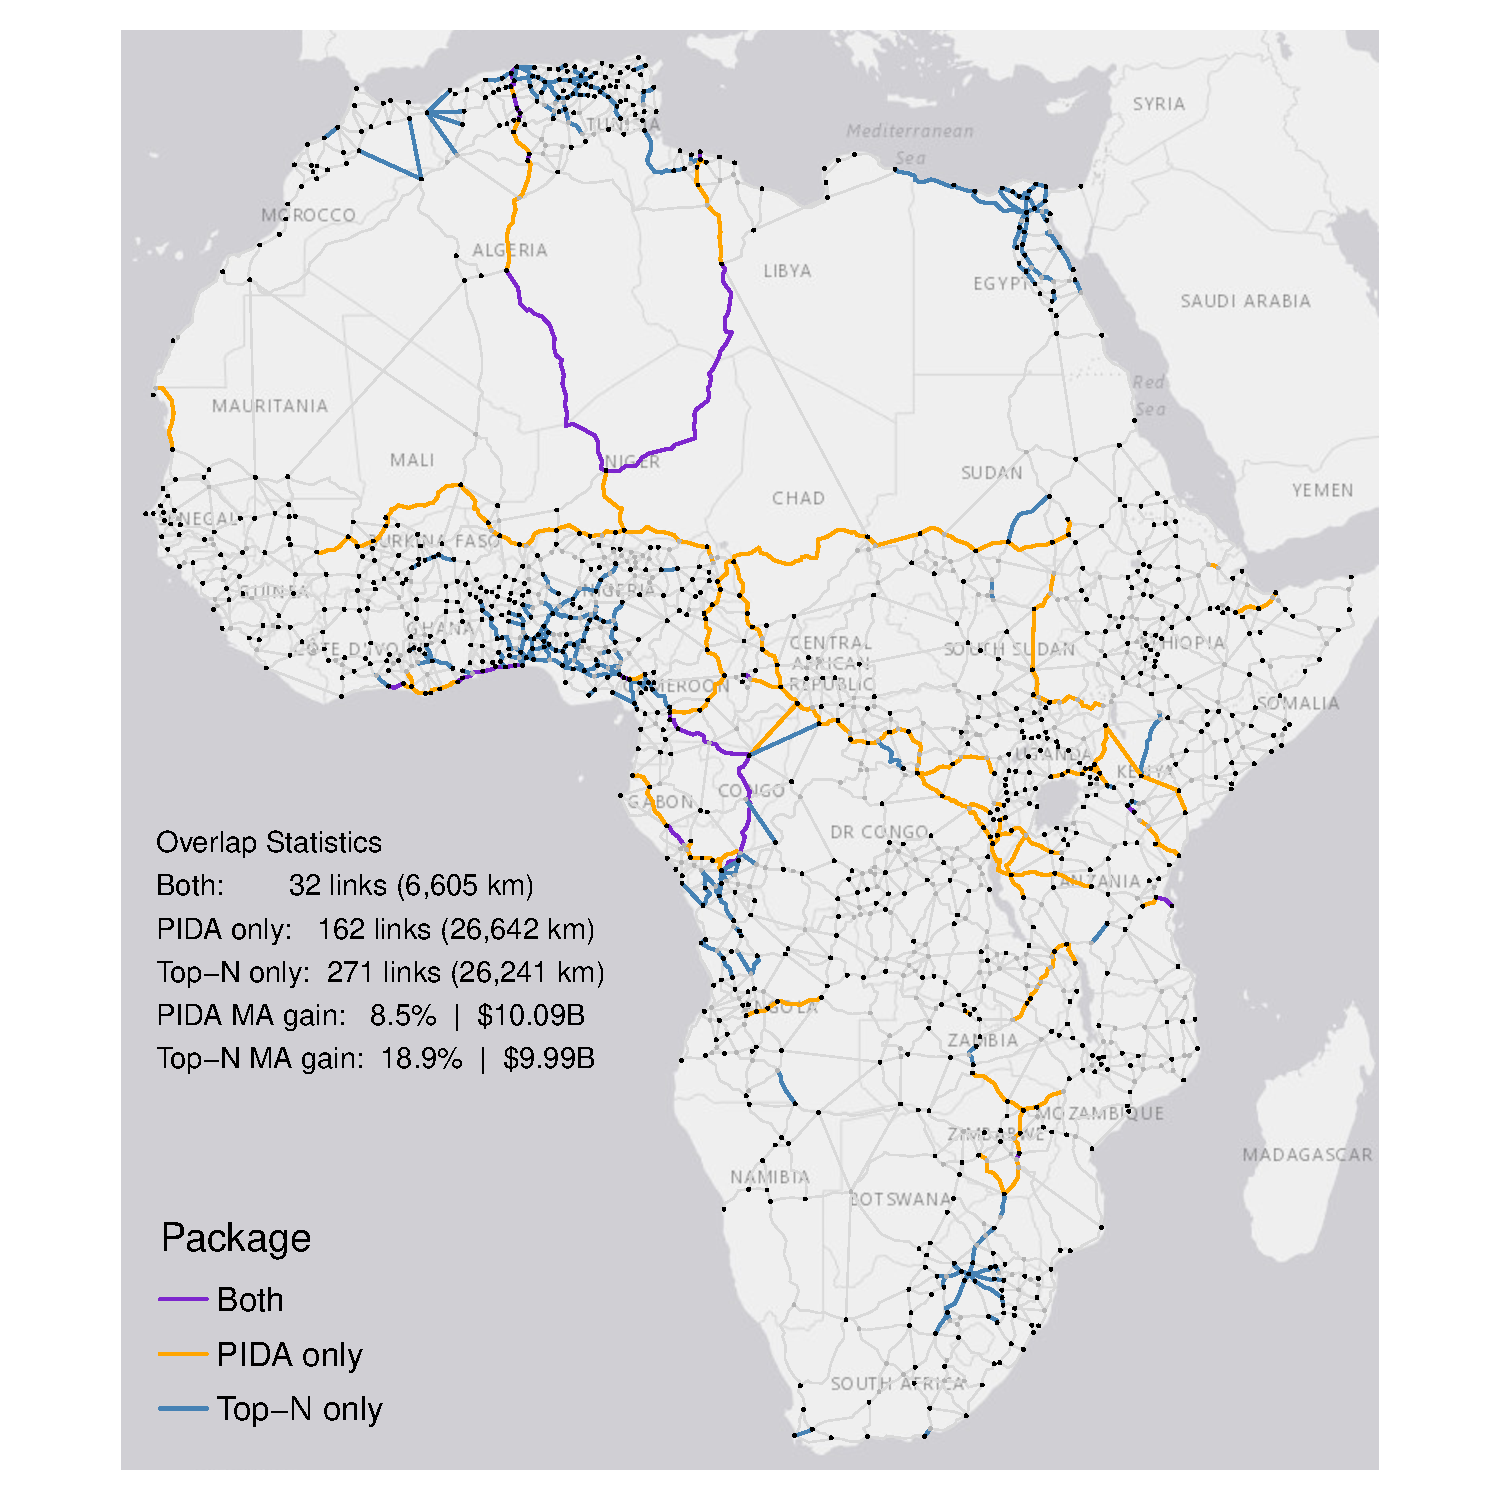
\includegraphics[width=0.48\textwidth, trim = {2cm 0 2cm 0}, clip]{../figures/transport_network/PIDA/trans_africa_network_PIDA_vs_top10B_consensus.pdf} &
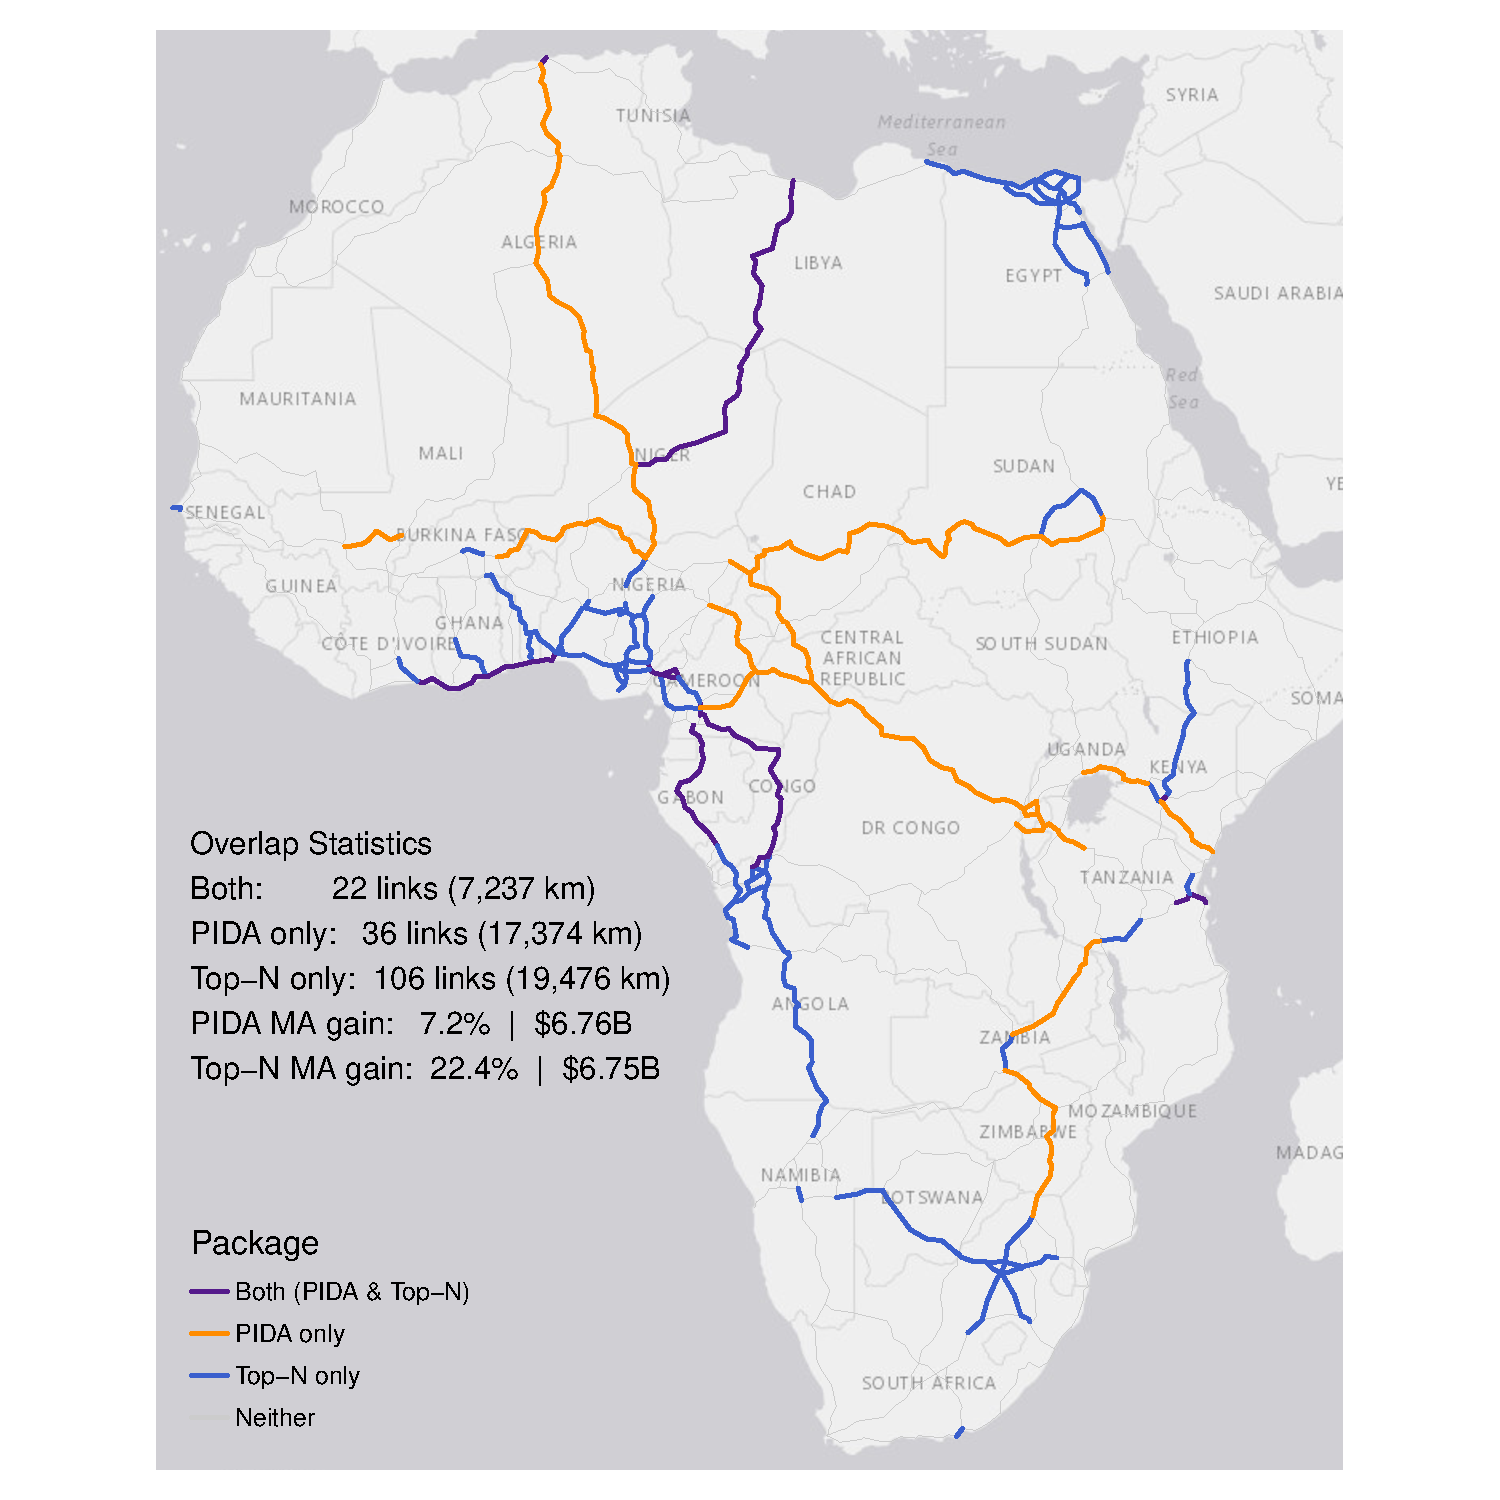
\includegraphics[width=0.48\textwidth, trim = {2cm 0 2cm 0}, clip]{../figures/transport_network/PIDA/PE_trans_african/trans_africa_network_PE_TA_PIDA_vs_topN_consensus.pdf} \\
\end{tabular}
}
\raggedright
\scriptsize
\emph{Notes:} Purple: links in both PIDA and the cost-matched top-N consensus benchmark. Orange: links in PIDA only. Blue: links in the top-N consensus benchmark only. The benchmark contains the highest-yielding links sorted by consensus \$/min/\$ until the cumulative cost matches the PIDA total on the respective network: \$10.1B on the full grid (left) vs.\ \$6.8B on the 330-edge trans-African network (right; only the subset of PIDA roads that fall on a 47-largest-port-city corridor is included). MA gains reported are frictionless joint percentages relative to the network's baseline. % \vspace{-1mm}
\end{figure}

%  The macroeconomic feasibility analysis (Table \ref{tab:MACAB}) yields that PIDA would be jointly profitable in PDV terms if it raises the macroeconomic growth rate by 0.06\% in the 4.1\% baseline-growth scenario or 0.09\% in the 3\% scenario. Comparing these to the 1.9--8.5\% MA gain implies a required MA-to-growth ratio of between 21:1 (frictions) and 142:1 (frictionless), comfortably below the 4:1 elasticity suggested by Table \ref{tab:MAregs} and the 2:1 elasticity of \citet{donaldson2016railroads}, even if costs overrun by a factor of two. \newline

% Overall, the PIDA package is decently efficient in PE terms, particularly its OSBP component, and substantially improves connectivity along major trans-African corridors. However, the cost-matched optimal benchmark in Figure \ref{fig:PIDA_vs_Top10B} suggests that reallocating spending from the more remote PIDA-only segments (notably in trans-Saharan and Central-African corridors) toward populated regions and crop belts in West Africa, the Horn of Africa, and Southern Africa would roughly double the package's frictionless MA return (8.5\%~$\to$~18.4\%), and could yield an order-of-magnitude improvement under frictions (1.9\%~$\to$~17.1\%). Targeted refinements to the PIDA pipeline---particularly broadening its OSBP component toward the full 31-edge programme, which delivers 3.6 percentage points of additional MA at minimal cost---could thus deliver outsized additional gains. A welfare-based assessment in general equilibrium is provided in \S\ref{sec:GE_PIDA} below. \newline

\subsection{General Equilibrium Evaluation} \label{sec:GE_PIDA}

To complement the PE assessment, I also evaluate PIDA against the welfare-maximising planner of \citet{fajgelbaum2020optimal} at exactly the PIDA-equivalent budget of $K_i = \$10.089$B USD'15. The natural comparison set is the trans-African routes network introduced in Section \ref{ss:TAGE}, connecting the 47 largest African port-cities along their fastest routes.  \newline % Using the same geometric-coverage matching as in Figure \ref{fig:PIDA_vs_Top10B}, 58 of these 330 edges ($\approx 17.6\%$) coincide with a PIDA project. \newline

As established in Section \ref{sec:GE}, trans-African connections plausibly exhibit weak congestion and IR ($\gamma^\ast = \beta^2/\gamma$). Figure \ref{fig:PIDA_GE_main} below therefore reports the IR case; the standard-congestion (DR) case is provided in Figure \ref{fig:PIDA_GE_DR}. For each planner I show the utilitarian ($\rho = 0$) and inequality-averse ($\rho = 2$) social welfare functions, and both the Armington baseline ($\sigma = 3.8$) and the lower elasticity ($\sigma = 2$) consistent with the MA gain of 1 ($\theta = \sigma - 1$; Footnote~\ref{fn:theta_sigma}). Frictions are intentionally omitted in all runs: as established in Section \ref{ss:TAGE}, border frictions have only minor effects on the GE-optimal allocation. The OSBP component, whose effect is precisely identified in the PE analysis above, is thus left aside in the GE counterfactual. \newline

Figure \ref{fig:PIDA_GE_main} overlays the PIDA-flagged subset of the trans-African network (navy dotted) on each planner's optimal upgrading allocation. All four IR variants spend the full \$10.089B budget on upgrading between 38.0K and 40.7K\,km. The spatial pattern is broadly consistent with Figure \ref{fig:TA_GE_Comp_IRS} where equivalent planners spend a \$15B budget on the same network. \newline % across the four variants: the highest-intensity upgrades fall on the Lagos--Abidjan and Lagos--Kano corridors, the Nairobi--Mombasa--Dar es Salaam axis, the trans-Saharan north--south spine, and the southern African network around Johannesburg and Cape Town. \newline

\begin{figure}[h!] \vspace{-4mm}
\caption{\label{fig:PIDA_GE_main} Welfare-Maximising GE Investments at \$10.1B with PIDA Overlay (IR Planner)}
\vspace{2mm}
\resizebox{\textwidth}{!}{
\begin{tabular}{@{}c@{}c@{}}
%\textbf{Standard ($\rho = 0$), $\sigma = 3.8$} & \textbf{Inequality-averse ($\rho = 2$), $\sigma = 3.8$} \\
%WG: 0.40\%  |  CG: 0.48\%  |  MA: 20.4\% &
%WG: 0.18\%  |  CG: 0.26\%  |  MA: 21.3\% \\
% PIDA-share: 13.6\% & PIDA-share: 13.6\% \\
Non-Inequality Averse Planner, $\sigma = 3.8$ & Inequality Averse Planner, $\sigma = 3.8$ \\
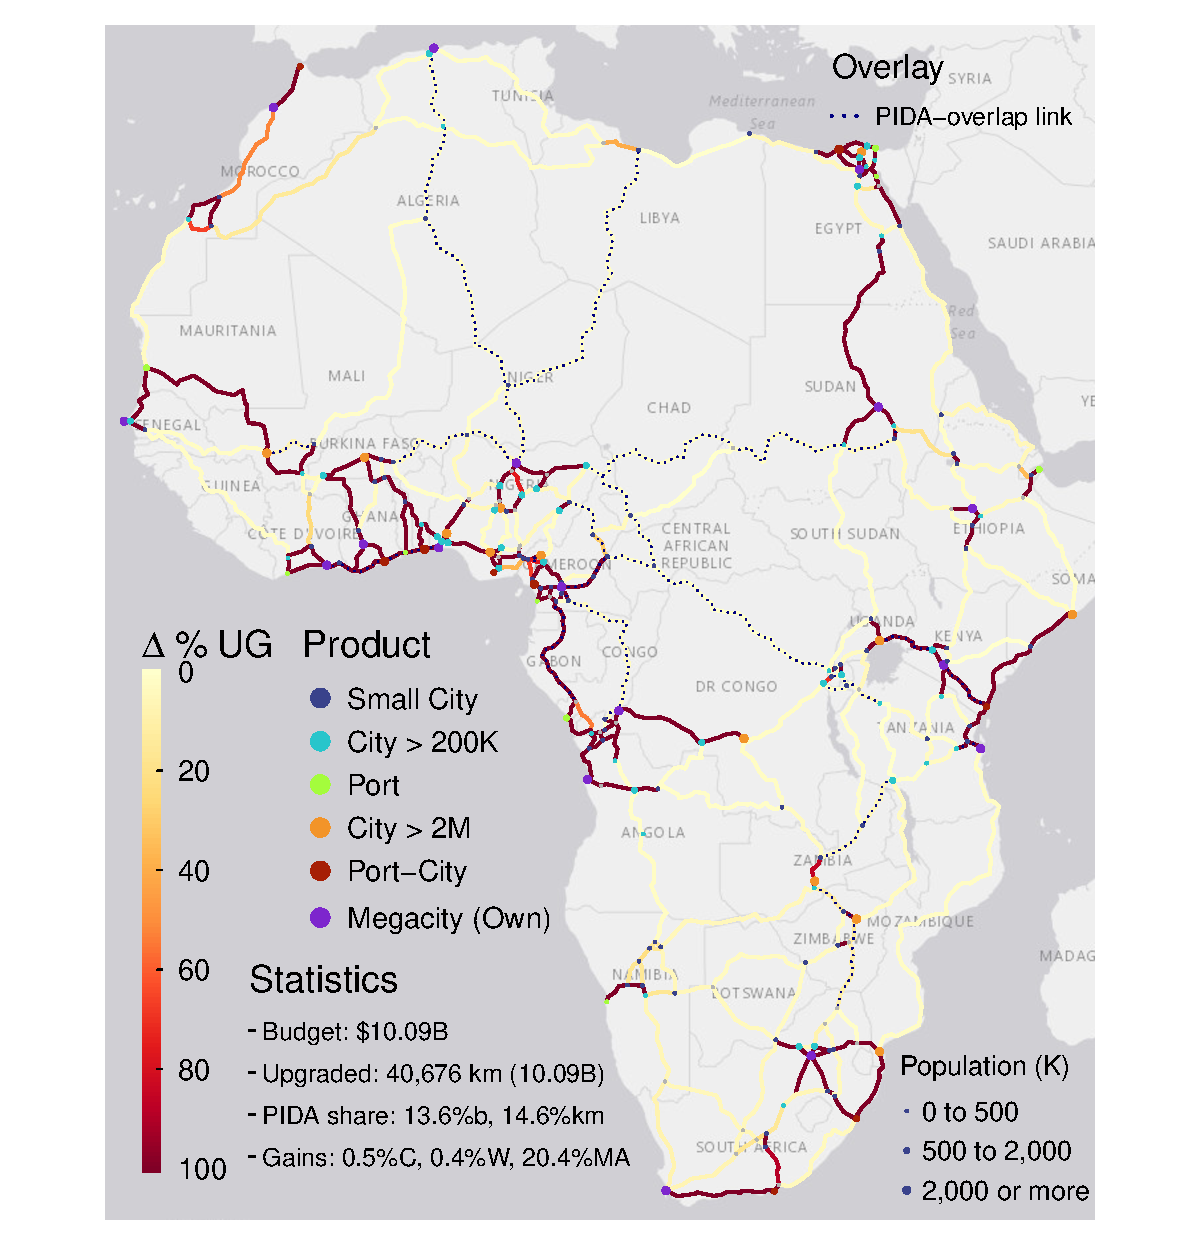
\includegraphics[width=0.48\textwidth, trim = {2cm 0 0.5cm 0}, clip]{../figures/transport_network/PIDA/GE_trans_african/trans_africa_network_GE_22g_10089m_fixed_cgc_irs_na_sigma3.8_rho0_duality_julia_perc_ug_with_PIDA.pdf} &
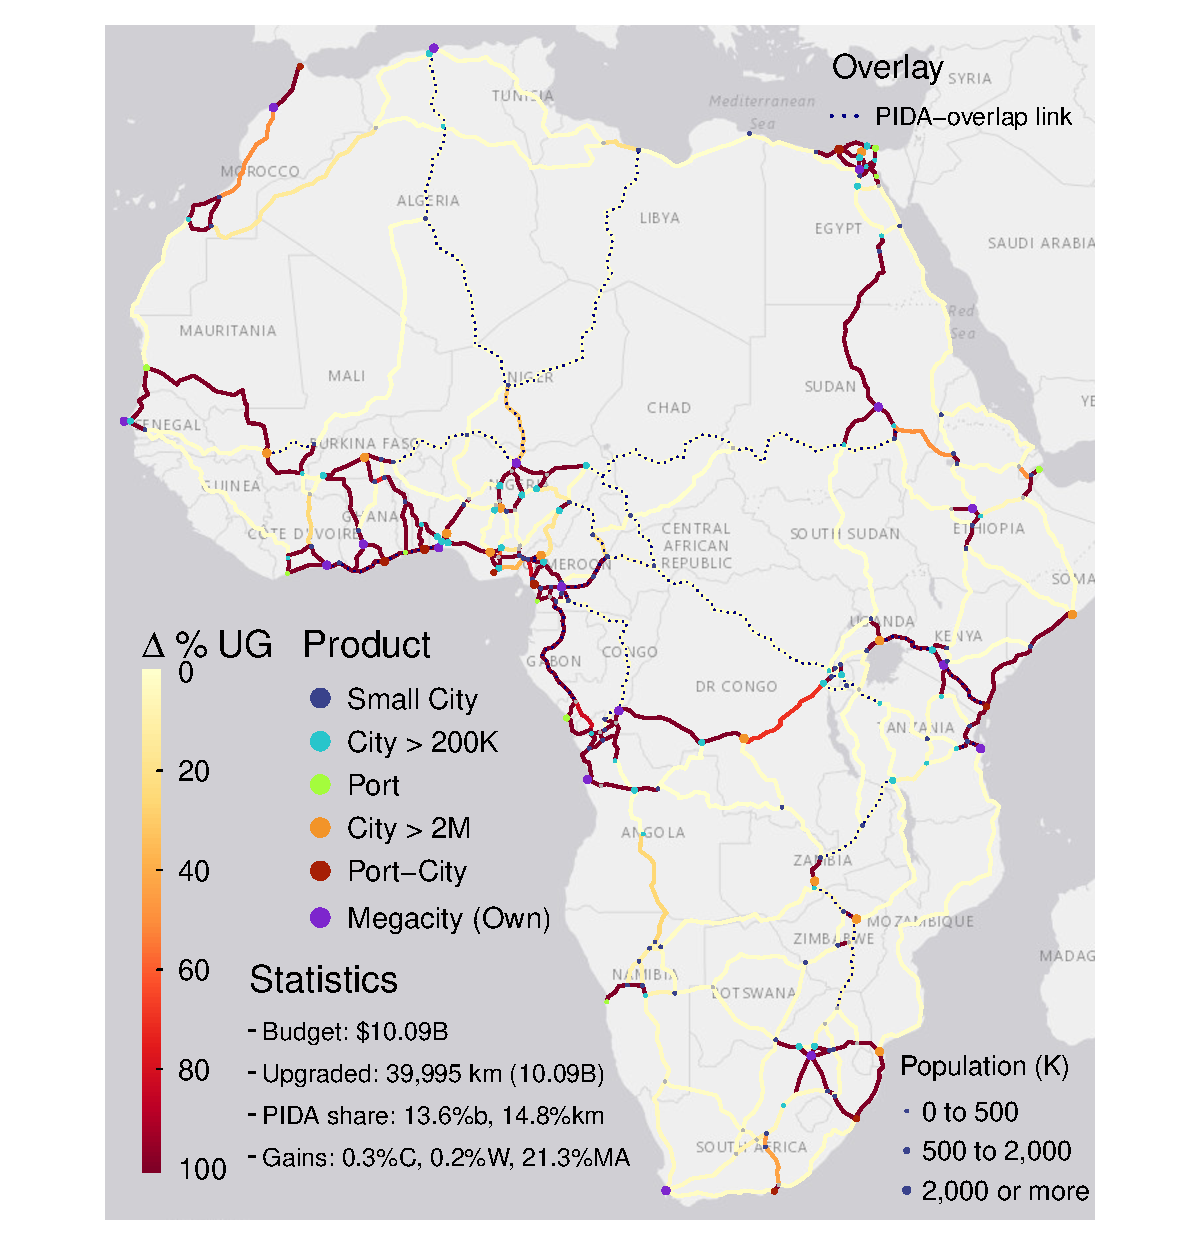
\includegraphics[width=0.48\textwidth, trim = {2cm 0 0.5cm 0}, clip]{../figures/transport_network/PIDA/GE_trans_african/trans_africa_network_GE_22g_10089m_fixed_cgc_irs_na_sigma3.8_rho2_duality_julia_perc_ug_with_PIDA.pdf} \\
%\textbf{Standard ($\rho = 0$), $\sigma = 2$} & \textbf{Inequality-averse ($\rho = 2$), $\sigma = 2$} \\
%WG: 2.78\%  |  CG: 3.87\%  |  MA: 20.1\%   &
%WG: 2.40\%  |  CG: 3.45\%  |  MA: 19.9\%  \\
%PIDA-share: 14.0\% & PIDA-share: 15.5\% \\ 
Non-Inequality Averse Planner, $\sigma = 2$ & Inequality Averse Planner, $\sigma = 2$ \\
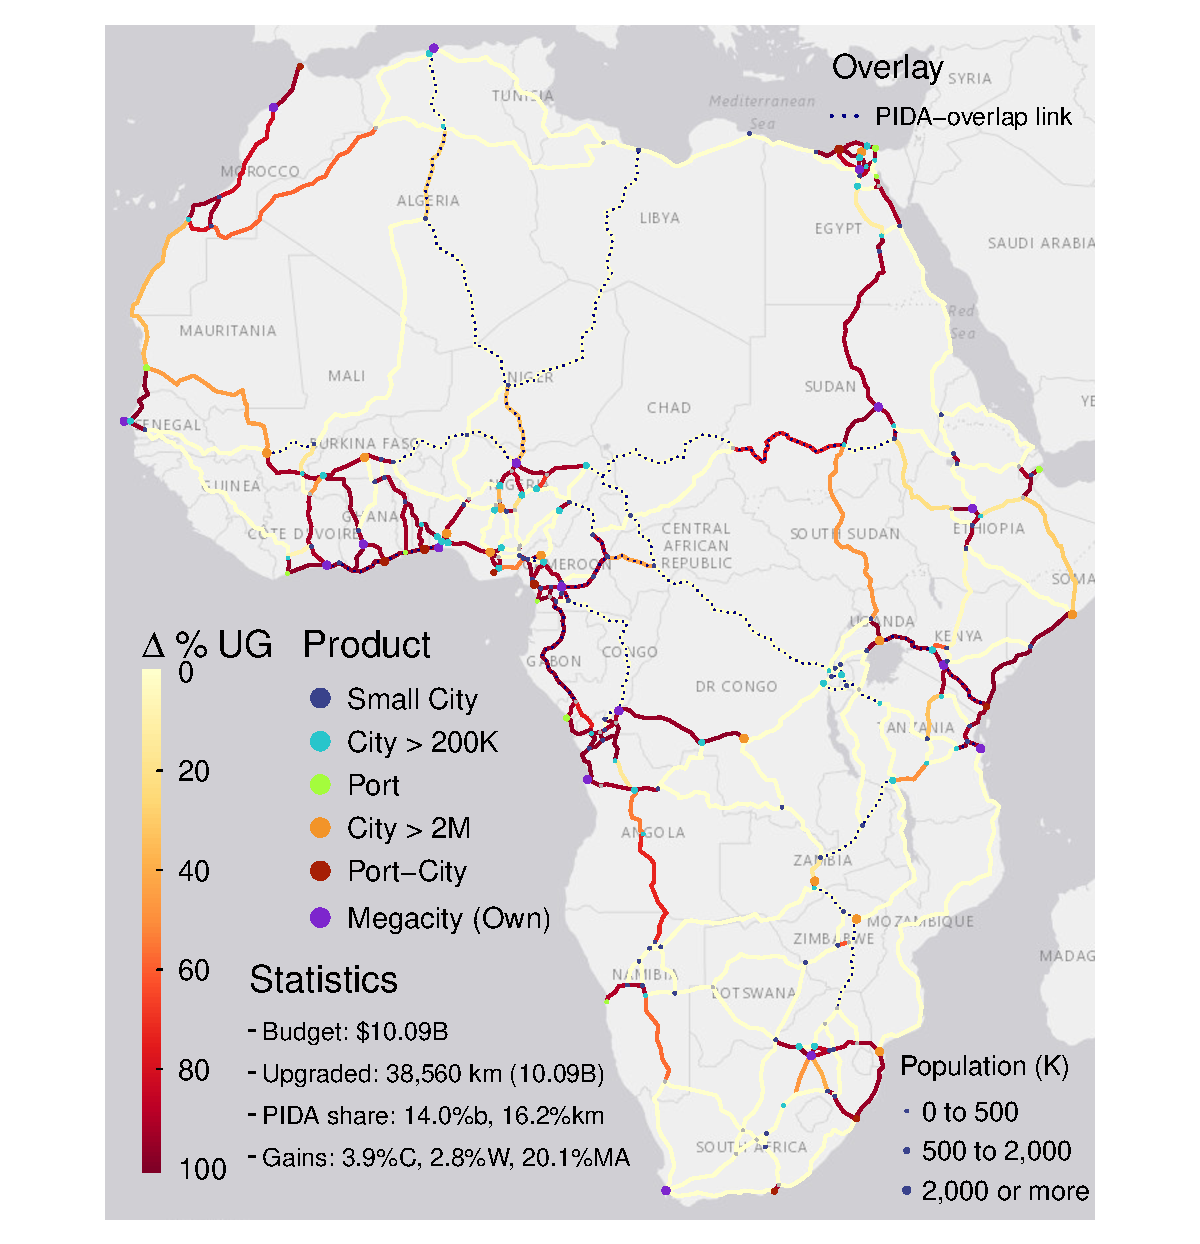
\includegraphics[width=0.48\textwidth, trim = {2cm 0 0.5cm 0}, clip]{../figures/transport_network/PIDA/GE_trans_african/trans_africa_network_GE_22g_10089m_fixed_cgc_irs_na_sigma2.0_rho0_duality_julia_perc_ug_with_PIDA.pdf} &
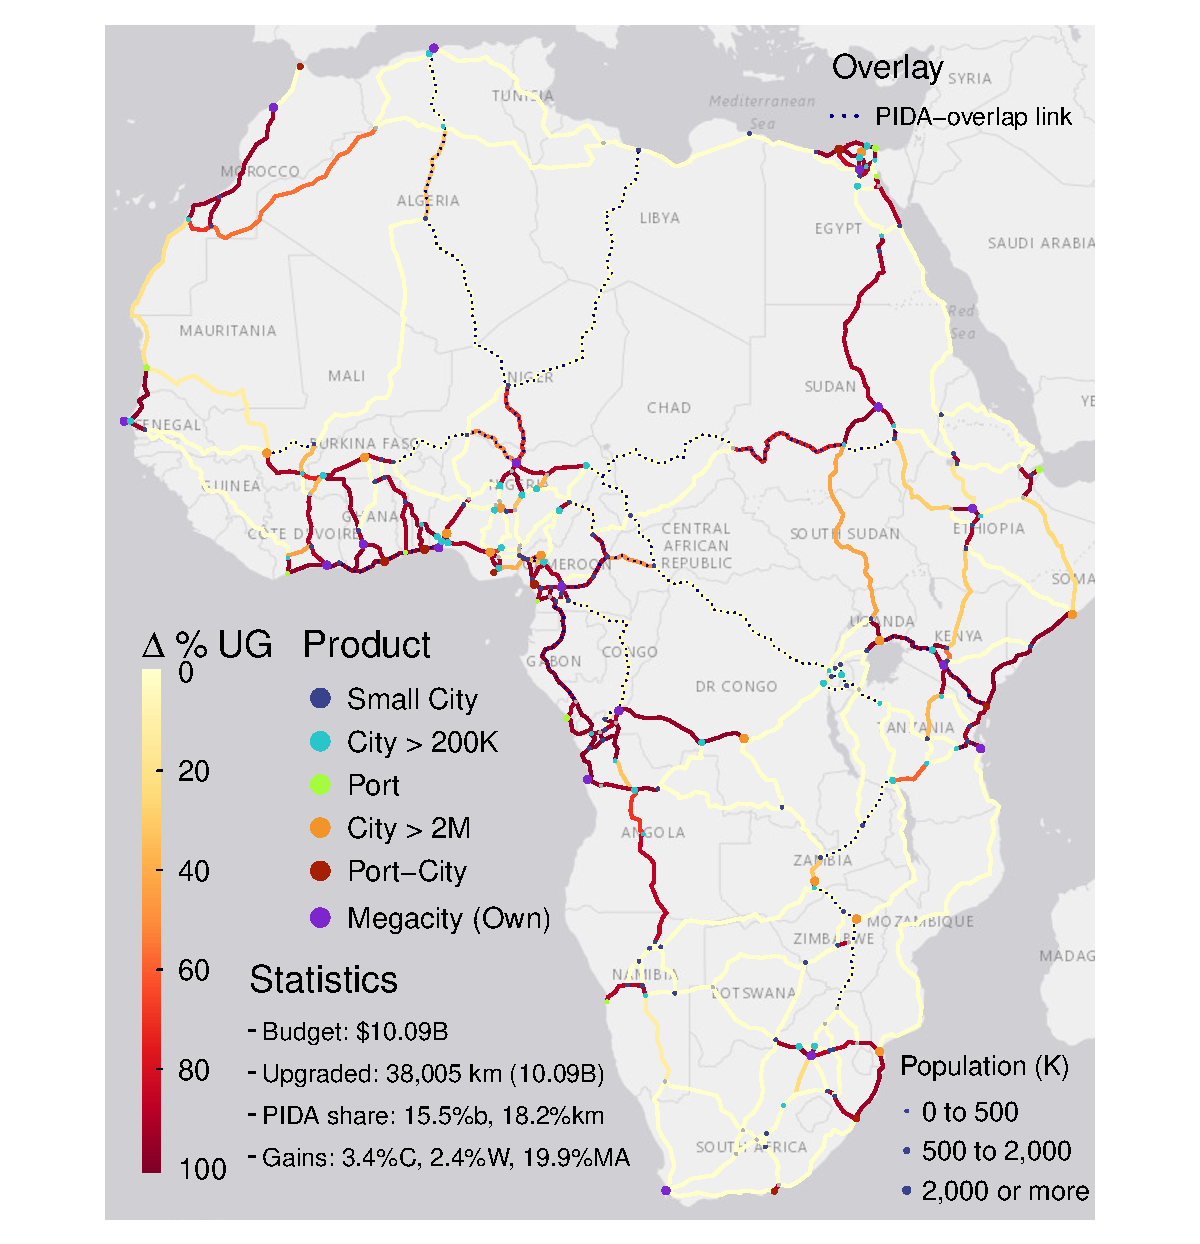
\includegraphics[width=0.48\textwidth, trim = {2cm 0 0.5cm 0}, clip]{../figures/transport_network/PIDA/GE_trans_african/trans_africa_network_GE_22g_10089m_fixed_cgc_irs_na_sigma2.0_rho2_duality_julia_perc_ug_with_PIDA.pdf} \\
\end{tabular}
}
\raggedright
\scriptsize
\emph{Notes:} Each panel shows the welfare-maximising allocation of a \$10.089B infrastructure budget (the PIDA-equivalent cost) on the condensed trans-African network connecting the 47 largest port-cities (330 corridor segments), under increasing returns to infrastructure ($\gamma^\ast = \beta^2/\gamma$). Columns vary the social-welfare function (utilitarian vs.\ inequality-averse $\rho = 2$); rows vary the Armington elasticity ($\sigma = 3.8$ top, $\sigma = 2$ bottom). Yellow-to-red intensity indicates the fractional upgrade ($\Delta\%$ UG) chosen by the planner; navy dotted lines overlay the 58 trans-African links matched to PIDA projects via geometric coverage (cf.\ Fig.\ \ref{fig:PIDA_vs_Top10B}). WG = aggregate welfare gain, CG = consumption gain, MA = market-access gain on the resulting network; PIDA-share is the fraction of the optimal budget that falls on the PIDA-overlap subset (network edge-count floor: $58/330 = 17.6\%$). % Frictions are omitted (\S\ref{ss:TAGE} shows their effect on the allocation shape is minor).
The DR case is reported in Appendix Figure \ref{fig:PIDA_GE_DR}. \vspace{-5mm}
\end{figure}

The headline finding is that the IR planners route between 13.6\% and 15.5\% of their budgets to PIDA corridors. Set against the network edge-count floor of $58/330 = 17.6\%$, this indicates that the welfare-maximising planner mildly under-weights PIDA's selection relative to the rest of the strategic network. 
The overlap rises modestly with lower trade elasticity ($\sigma = 2$: 14.0\%--15.5\%) because less-substitutable goods push the planner to spread spending more evenly across the strategic-corridor system. The inequality-averse planner ($\rho = 2$) yields very similar PIDA-overlap shares, suggesting PIDA's selection criteria incorporate some implicit weight on remote regions. \newline

In terms of both welfare and MA gains achieved, the GE-optimal allocation outperforms PIDA substantially. The frictionless MA gain on the resulting GE network is 19.9\%--21.3\% across the four IR variants, against PIDA's PE-derived gain of 7.3\% on the same 330-edge trans-African network (8.5\% on the full continental one)---the welfare-optimal use of the budget thus nearly triples the MA gain of PIDA's corridors.\footnote{The two figures are not on an identical footing: the GE planner deploys the full \$10.089B on the 330-edge network, whereas PIDA's projects on those same corridors cost only \$6.76B (the remaining \$3.3B of PIDA road lies off the 47-city corridor system; cf.\ Figure \ref{fig:PIDA_vs_Top10B}). The gap therefore reflects both a superior \textit{allocation} of spending and the planner's freedom to concentrate the entire PIDA-equivalent budget on the strategic network. The cost-matched PE comparison in Figure \ref{fig:PIDA_vs_Top10B}, which holds the budget fixed at \$6.75B, isolates the pure allocation effect and still finds a $3.1\times$ MA improvement. The PE market-access gain ($\theta$) and the GE welfare allocation ($\sigma$) are governed by the same elasticity primitive ($\theta = \sigma - 1$; Footnote~\ref{fn:theta_sigma}), so these figures are consistent under $\sigma = 2$.} Aggregate welfare gains range from 0.18\% (IR, $\sigma = 3.8$, $\rho = 2$) to 2.78\% (IR, $\sigma = 2$, $\rho = 0$); lower trade elasticity raises the gains by an order of magnitude because each city's good is more uniquely valuable when substitution is harder, amplifying the welfare benefit of upgrading any given corridor. Inequality aversion typically lowers aggregate welfare by a few tenths of a percentage point as the planner trades off mean for variance. \newline

Putting PE and GE together, PIDA emerges as a partially-targeted but materially under-optimal package. A planner with the same \$10.089B budget optimally allocated would upgrade the Lagos--Abidjan coastal corridor, the Mombasa--Nairobi axis, the trans-Saharan north--south spine, and several southern African links that PIDA underweights---roughly doubling the full-grid MA return (8.5\%~$\to$~18.4\%, against the PE-optimal benchmark) and nearly triple it on the strategic network (7.3\%~$\to$~19.9--21.3\%, against the GE-optimal allocation), while unlocking substantially larger welfare gains ranging from 0.18\% to 2.78\% depending on the assumed trade elasticity and social-welfare function. Combining this re-allocation with the OSBP component (3.6 pp. PE gain) would push the joint return higher still. \newline

An important caveat tempers the normative reading of this efficiency gap. The planners in this paper only maximize aggregate welfare or MA. But many of the PIDA corridors that the optimal allocation would deprioritize---trans-Saharan links, Central-African connections, and roads serving landlocked and fragile states such as Chad, the Central African Republic, and South Sudan---advance regional integration under the AfCFTA, support state presence and humanitarian access in remote areas, and must remain politically feasible across the African Union's member governments with divergent national interests. %%That planned projects score lower on aggregate market-access efficiency may be precisely because they pursue these non-modelled goals. 
The gap is therefore better read not as evidence of poor planning, but as a measure of the price---in forgone MA---that the continent pays for connectivity to its most remote and fragile regions and for the political viability of a six-decade, multi-country investment programme. Quantifying that price is itself valuable policy information: the figures above tell decision-makers roughly how much aggregate MA is being traded for the broader integration and equity objectives the welfare model does not capture, and where the two objectives are most complementary and least in tension. % \newline



% \newpage

\section{Conclusion} % Summary and   and Policy Recommendations

This paper rigorously examines Africa's continental road network and characterizes optimal investments into it in partial and general equilibrium (PE and GE). Africa has 1.6 million km of non-residential roads ($\sim$30\% paved), with a network route efficiency of 0.68 (vs.\ 0.84 for the US). Cross-border frictions are severe: the median border crossing is equivalent to 1043km of road distance, inducing aggregate MA losses of 26-78\%. \newline 

In PE, I find that upgrading all links to $\geq$100km/h yields a 42\% MA gain---far exceeding the 5.5\% from new links alone---at an estimated cost of \$106B. Building proposed new links costs \$56B. Combining both, consensus investment packages targeting high-return links cost \$17-61B and yield 19-38\% MA gains, which are macroeconomically feasible under plausible assumptions. Border frictions reduce these gains substantially, particularly for remote and transnational links. \newline 

In GE, welfare-maximizing planners with \$35B focus on connecting large cities and ports to surrounding areas, with about 30\% of spending on new links. An inequality-averse planner invests more in poorer Central African and Horn of Africa regions. Under increasing returns to infrastructure, planners invest more in road upgrading and less in new construction, increasing welfare gains. Trans-African planners with \$15B primarily improve regional connectivity; making central African cross-continental links a priority requires unrealistically low trade elasticities ($\sigma = 1.5$) combined with inequality aversion. Border frictions further reduce investments along these links. \newline

Benchmarking the African Union's PIDA pipeline against these frameworks (\S\ref{sec:PIDAeval}) reveals a partially-targeted but materially under-optimal package. At its \$10.1B budget, PIDA delivers an 8.5\% frictionless MA gain against 18.4\% for the cost-matched PE-optimal benchmark, and the welfare-maximizing GE planner directs only 13.6--15.5\% of the same budget to PIDA-flagged corridors---slightly below the 17.6\% pro-rata edge-count share. Reallocating spending from remote trans-Saharan and Central-African segments toward the Lagos--Abidjan, Mombasa--Nairobi, and southern-African corridors, and broadening the one-stop-border-post component (an additional 3.6 percentage points of MA at minimal cost), would roughly double the package's market-access return. \newline

The overarching finding is that trans-African roads are neither MA nor welfare maximizing compared to improved local connectivity in populated areas or between nearby cities and coastal ports. This is especially true under border frictions, which reduce the value of trans-African links. Yet, these links are essential for trans-African trade under AfCFTA to pick up. A general policy recommendation is thus to prioritize regional connectivity improvements, reduce border frictions, and invest in trans-African roads along specific high-yield corridors. The graphical results provided in the paper and appendix should be helpful in prioritizing continental and regional investments, with detailed data and results available \href{https://github.com/SebKrantz/OptimalAfricanRoads}{on GitHub}. The multi-level approach combining routing engines, PE, and GE analysis can also be adapted to examine specific regions---as demonstrated for the \href{https://www.dropbox.com/scl/fi/67nwybv21px11r5bnqoek/optimal_CEMAC_roads.pdf?rlkey=x7q71wzfxjddtushojo4w4rec&e=1&dl=0}{CEMAC region} as part of a World Bank regional infrastructure assessment. The \href{https://github.com/OptimalTransportNetworks/OptimalTransportNetworks.jl}{Julia library} and \href{https://github.com/SebKrantz/OptimalAfricanRoads}{reproducibility package} should be useful in this regard.

% \vspace{1cm}
\newpage

\bibliographystyle{apacite}
\bibliography{quant_spatial_econ} 
\newpage
\section*{Appendix}
\setcounter{table}{0}
\renewcommand{\thetable}{A\arabic{table}}
\setcounter{figure}{0}
\renewcommand{\thefigure}{A\arabic{figure}}

% === PIDA GE robustness: DR (standard congestion) counterpart of main figure ===

\begin{figure}[H] \vspace{-2mm}
\caption{\label{fig:PIDA_GE_DR} Welfare-Maximising GE Investments at \$10.1B with PIDA Overlay (DR Planner)}
\vspace{2mm}
\resizebox{\textwidth}{!}{
\begin{tabular}{@{}c@{}c@{}}
%\textbf{Standard ($\rho = 0$), $\sigma = 3.8$} & \textbf{Inequality-averse ($\rho = 2$), $\sigma = 3.8$} \\
%WG: 0.08\%  |  CG: 0.10\%  |  MA: 19.8\% &
%WG: 0.04\%  |  CG: 0.06\%  |  MA: 20.7\% \\
% PIDA-share: 13.9\% & PIDA-share: 14.1\% \\
Non-Inequality Averse Planner, $\sigma = 3.8$ & Inequality Averse Planner, $\sigma = 3.8$ \\
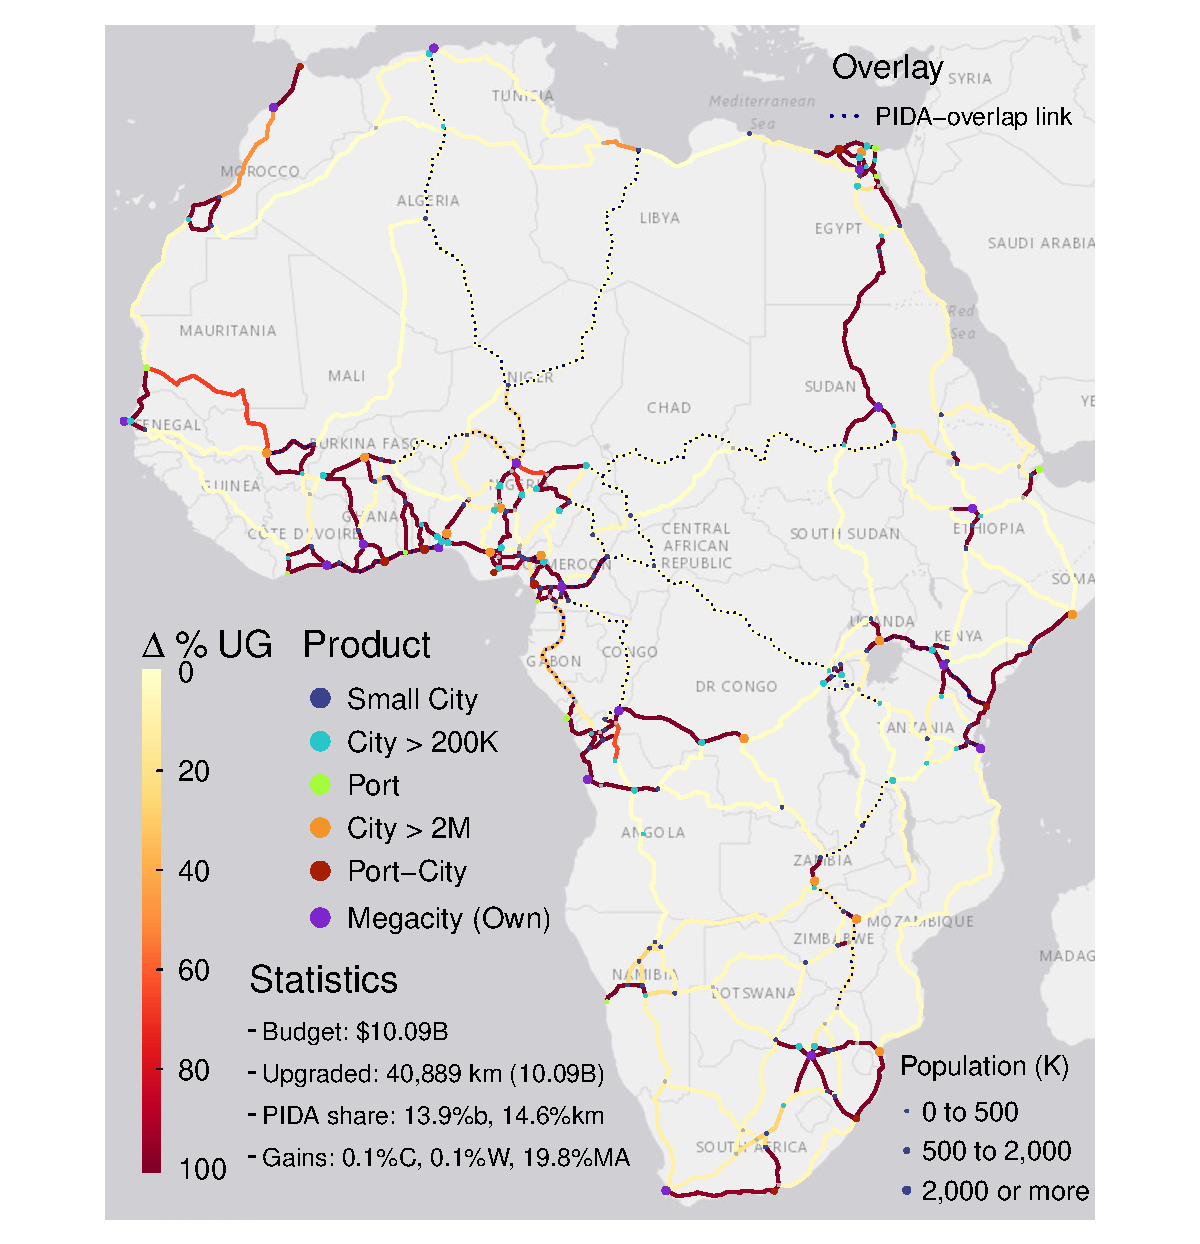
\includegraphics[width=0.48\textwidth, trim = {2cm 0 0.5cm 0}, clip]{../figures/transport_network/PIDA/GE_trans_african/trans_africa_network_GE_22g_10089m_fixed_cgc_sigma3.8_rho0_duality_julia_perc_ug_with_PIDA.pdf} &
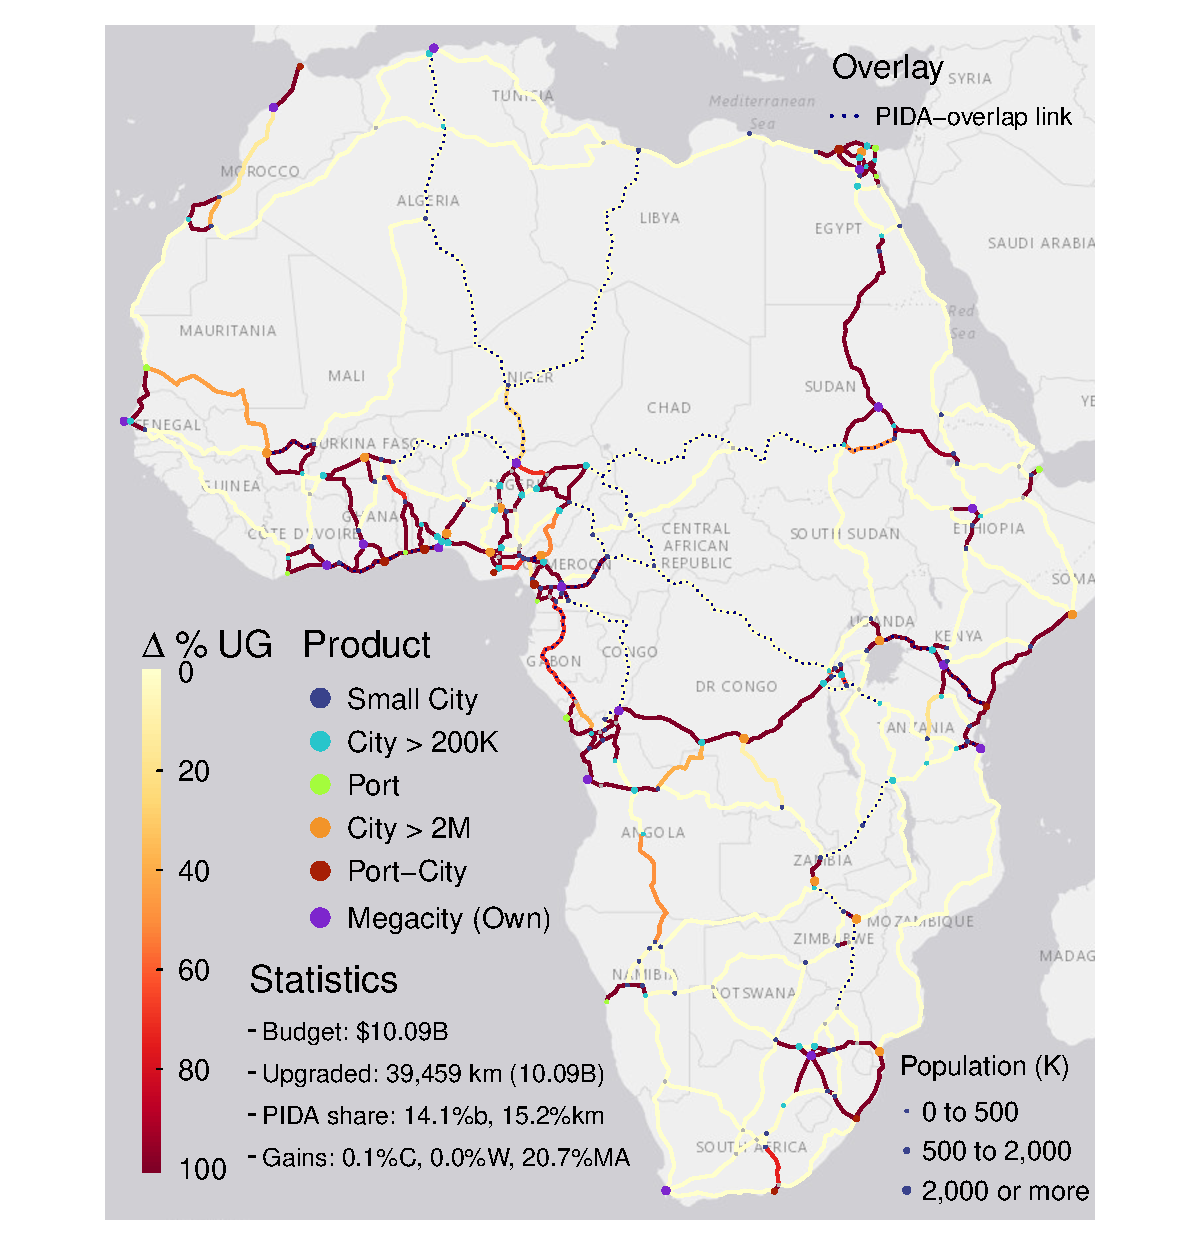
\includegraphics[width=0.48\textwidth, trim = {2cm 0 0.5cm 0}, clip]{../figures/transport_network/PIDA/GE_trans_african/trans_africa_network_GE_22g_10089m_fixed_cgc_sigma3.8_rho2_duality_julia_perc_ug_with_PIDA.pdf} \\
%\textbf{Standard ($\rho = 0$), $\sigma = 2$} & \textbf{Inequality-averse ($\rho = 2$), $\sigma = 2$} \\
%WG: 1.11\%  |  CG: 1.52\%  |  MA: 20.8\%   &
%WG: 0.69\%  |  CG: 0.99\%  |  MA: 21.1\%  \\
%PIDA-share: 15.4\% & PIDA-share: 16.1\% \\
Non-Inequality Averse Planner, $\sigma = 2$ & Inequality Averse Planner, $\sigma = 2$ \\
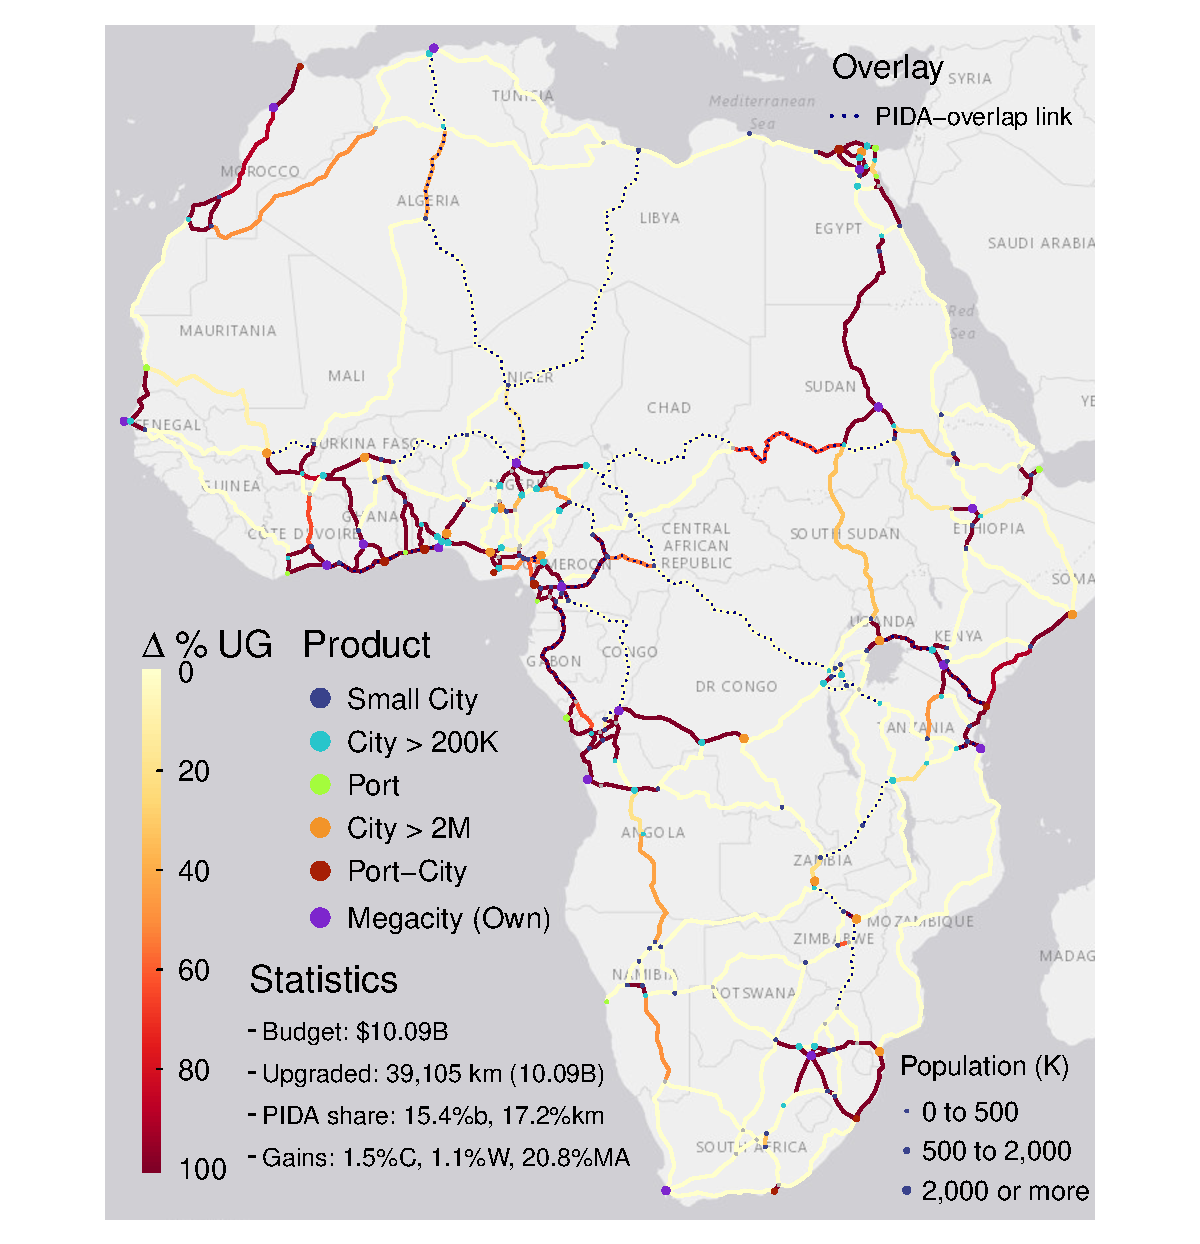
\includegraphics[width=0.48\textwidth, trim = {2cm 0 0.5cm 0}, clip]{../figures/transport_network/PIDA/GE_trans_african/trans_africa_network_GE_22g_10089m_fixed_cgc_sigma2.0_rho0_duality_julia_perc_ug_with_PIDA.pdf} &
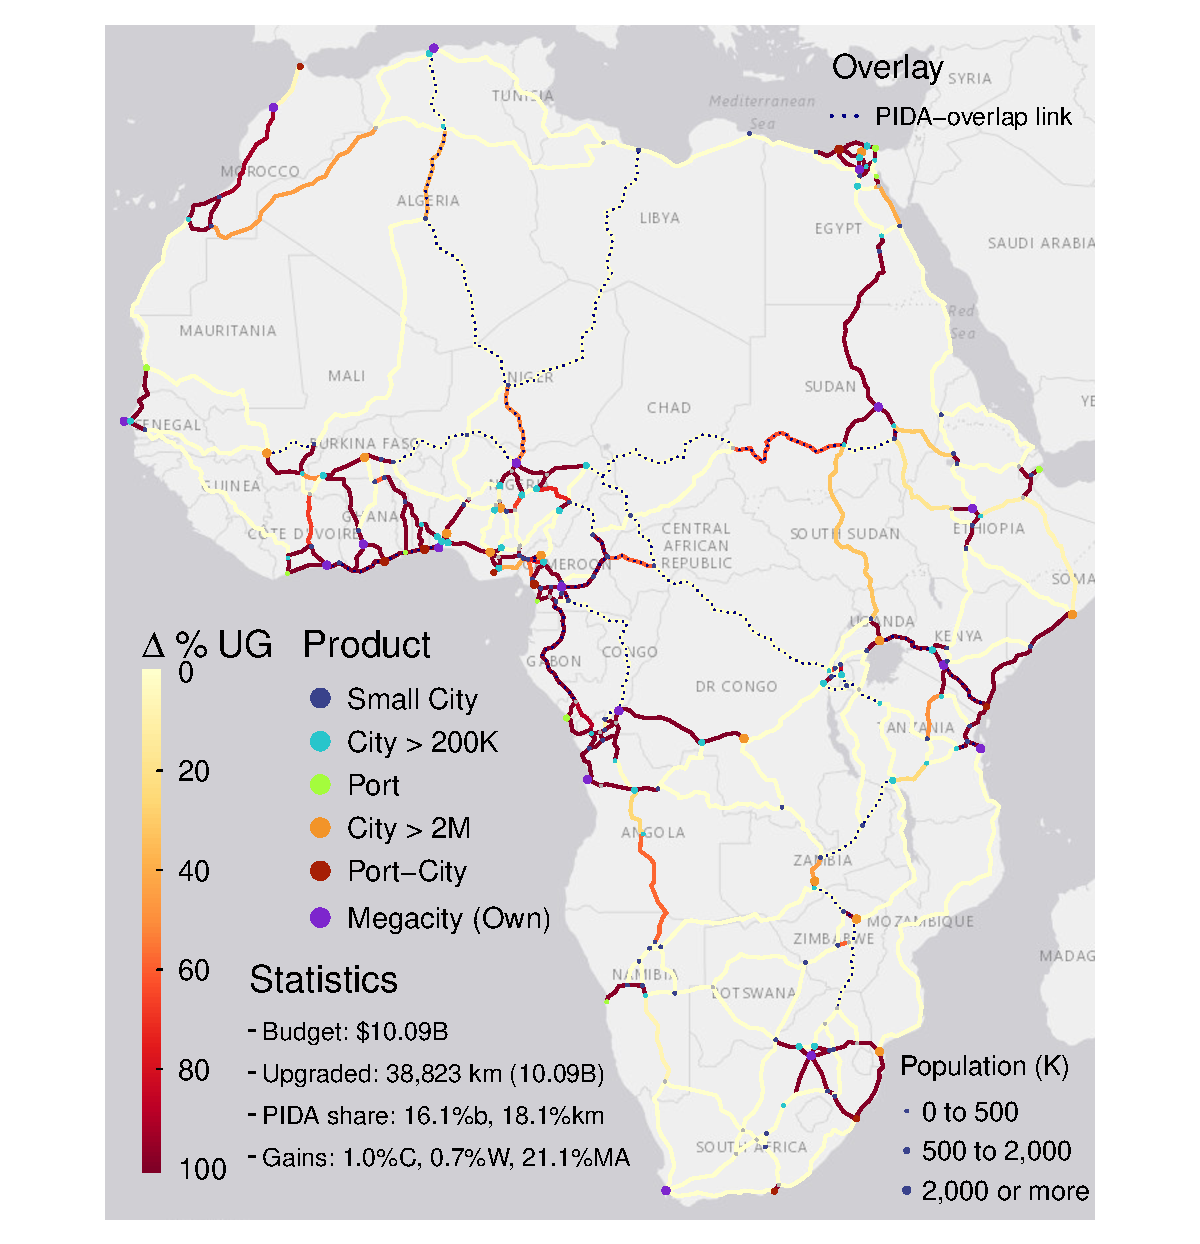
\includegraphics[width=0.48\textwidth, trim = {2cm 0 0.5cm 0}, clip]{../figures/transport_network/PIDA/GE_trans_african/trans_africa_network_GE_22g_10089m_fixed_cgc_sigma2.0_rho2_duality_julia_perc_ug_with_PIDA.pdf} \\
\end{tabular}
}
\raggedright
\scriptsize
\emph{Notes:} Counterpart of Figure \ref{fig:PIDA_GE_main} under the standard decreasing-returns (DR) congestion calibration $\gamma = \beta = 1$ derived from U.S. urban-congestion studies, rather than the IRS calibration $\gamma^\ast = \beta^2/\gamma$ used in the main figure. The spatial allocation is qualitatively similar to IRS---highest-intensity upgrades fall on the same Lagos--Abidjan, Lagos--Kano, Nairobi--Mombasa, and trans-Saharan corridors---but aggregate welfare gains are substantially smaller (0.04\%--1.11\%, vs.\ 0.18\%--2.78\% under IRS); MA gains and the PIDA-overlap share are essentially unchanged. The pattern reinforces the broader paper finding that the IRS regime is the more realistic and welfare-favourable parameterisation for continental-scale African transport. \vspace{-1mm}
\end{figure}


% === Tables moved from main text ===

\begin{table}[H] % \vspace{-2mm}
\centering
\caption{\label{tab:OSM_Roads}African Roads (OSM April 2024)}
\vspace{2mm}
\begin{tabular}{lrrr}
  \toprule
Highway Tag & N & Length in km & Paved Length in km \\ 
  \midrule
motorway & 14,986 & 22,400 & 17,744 (79.2\%) \\ 
  trunk & 75,265 & 181,459 & 128,978 (71.1\%) \\ 
  primary & 124,547 & 252,047 & 136,452 (54.1\%) \\ 
  secondary & 158,674 & 365,939 & 97,904 (26.8\%) \\ 
  tertiary & 299,573 & 790,067 & 94,373 (12.0\%) \\ \midrule
  Total & 673,045 & 1,611,912 & 475,450 (29.6\%) \\
   \bottomrule
\end{tabular}
\end{table}


\begin{table}[h!] \vspace{-2mm}
\centering
\caption{\label{tab:TARIFFs} World Development Indicators: Tariffs Applied in 2020}
\vspace{2mm}
\begin{tabular}{lrrrrrrrr}
  \toprule
& \multicolumn{4}{c}{All Products} & \multicolumn{4}{c}{Manufactured Products} \\
Region/Income Status & SSR & SIP & TR & WTR &  SSR & SIP & TR & WTR \\
  \midrule
  OECD & 5.7 & 2.7 & 2.0 & 1.6 & 0.3 & 0.6 & 1.5 & 1.5 \\ 
  Non-OECD & 0.5 & 19.1 & 8.0 & 6.3 & 0.2 & 17.8 & 7.5 & 6.0 \\ \midrule
  High income & 4.3 & 4.7 & 3.0 & 2.6 & 0.2 & 3.0 & 2.6 & 2.4 \\ 
  Low income & 0.0 & 34.3 & 11.1 & 9.3 & 0.0 & 32.4 & 10.6 & 8.4 \\ \midrule
Europe \& Central Asia & 5.0 & 2.4 & 2.5 & 1.9 & 0.3 & 0.6 & 2.2 & 1.9 \\ 
  Latin America \& Caribbean & 0.0 & 19.2 & 8.0 & 6.7 & 0.0 & 17.7 & 7.5 & 6.6 \\ 
  South Asia & 0.6 & 28.6 & 10.6 & 8.8 & 0.6 & 27.8 & 10.2 & 9.9 \\ 
  Middle East \& North Africa & 0.8 & 9.3 & 6.4 & 5.1 & 0.1 & 8.8 & 5.6 & 4.8 \\ 
  Sub-Saharan Africa & 0.1 & 33.9 & 10.8 & 8.2 & 0.1 & 32.5 & 10.5 & 7.6 \\ \midrule
  All Africa wtd. GDP PPP & 0.0 & 26.9 & 11.2 & 8.7 & 0.0 & 26.1 & 9.0 & 7.6 \\ 
\bottomrule \\ [-0.9em]
      \multicolumn{8}{l}{SSR $=$ Share of Tariff Lines with Specific Rates (\%)} \\
   \multicolumn{8}{l}{SIP $=$ Share of Tariff Lines with International Peaks (\%)} \\
   \multicolumn{8}{l}{TR $=$ Tariff Rate, Applied, Simple Mean (\%)} \\
   \multicolumn{8}{l}{WTR $=$ Tariff Rate, Applied, Weighted Mean (\%)} 
\end{tabular}
\vspace{-2mm}
\end{table}


\begin{table}[H] % \vspace{-2mm}
\centering
\caption{\label{tab:DB_TAB} World Bank Doing Business: Trading Across Borders in 2019}
\vspace{2mm}
\begin{tabular}{lrrrrrrrr}
  \toprule
 & \multicolumn{4}{c}{Exporting} & \multicolumn{4}{c}{Importing} \\  & \multicolumn{2}{c}{USD} & \multicolumn{2}{c}{Hours} & \multicolumn{2}{c}{USD} & \multicolumn{2}{c}{Hours} \\
Region/Income Status & BC & DC & BC & DC & BC & DC & BC & DC \\ 
  \midrule
  OECD & 149.7 & 34.8 & 12.8 & 2.5 & 106.5 & 26.5 & 9.4 & 3.8 \\ 
  Non-OECD & 453.8 & 145.0 & 64.0 & 55.8 & 531.5 & 191.4 & 82.5 & 66.5 \\ \midrule
High income & 228.4 & 68.0 & 24.8 & 12.6 & 252.1 & 74.3 & 22.1 & 16.0 \\ 
  Low income & 528.8 & 197.1 & 84.1 & 78.9 & 670.7 & 348.0 & 125.9 & 124.3 \\ \midrule 
Europe \& Central Asia & 117.8 & 47.1 & 11.9 & 12.2 & 91.8 & 42.1 & 10.4 & 11.2 \\ 
  South Asia & 310.6 & 157.9 & 53.4 & 73.7 & 472.9 & 261.7 & 85.7 & 93.7 \\ 
  Latin America \& Caribbean & 513.2 & 99.5 & 55.7 & 36.4 & 625.3 & 106.5 & 55.8 & 44.3 \\ 
  Middle East \& North Africa & 447.0 & 239.7 & 54.1 & 63.1 & 526.0 & 261.8 & 97.3 & 72.4 \\ 
  Sub-Saharan Africa & 603.1 & 172.5 & 97.1 & 71.9 & 690.6 & 287.2 & 126.2 & 96.1 \\ \midrule
  All Africa wtd. GDP PPP & 628.9 & 178.8 & 89.3 & 80.5 & 717.6 & 459.6 & 167.9 & 123.9 \\ 
   \bottomrule \\ [-0.9em]
      \multicolumn{8}{l}{DC $=$ Documentary Compliance, BC $=$ Border Compliance} 
\end{tabular}
\end{table}


\begin{table}[H] % \vspace{-2mm}
\centering
\caption{\label{tab:ROCKS} Road Building Costs: Road Costs Knowledge System (ROCKS) - 2018 Update}
\vspace{2mm}
\begin{tabular}{lrrrrr}
  \toprule
Work Type & N & Length (km) & Cost (M\$'15) & Cost/km \\ 
  \midrule
 \multicolumn{5}{l}{\textit{Continental Africa}} \\ 
    New 1L Road & 1 & 99.0 & 21.15 & 0.214 \\ 
 New 2L Highway & 4 & 122.0 & 59.53 & 0.611 \\ 
  \midrule  \multicolumn{5}{l}{\textit{All Low and Lower-Middle Income Countries}} \\ 
  New 1L Road & 6 & 59.5 & 7.65 & 0.135 \\ 
  New 2L Highway & 6 & 84.5 & 44.09 & 0.611 \\ 
  New 4L Expressway & 1 & 84.8 & 328.08 & 3.869 \\ \midrule
 \multicolumn{5}{l}{\textit{All Countries}} \\ 
  New 2L Highway & 7 & 50.0 & 43.03 & 0.682 \\     
  New 4L Expressway & 24 & 74.9 & 213.01 & 5.152 \\ 
   \bottomrule  \\ [-0.9em]
\multicolumn{5}{l}{\parbox{0.7\textwidth}{\footnotesize
\textit{Notes:} Statistics are aggregated across projects using the median. Costs are in millions of 2015 USD. The raw costs in current USD were deflated at their project end date using the US GDP deflator with base year 2015.  }}
\end{tabular}
\end{table}


\begin{table}[H]
\centering
\caption{\label{tab:ROCKS_UG} Road Upgrading Costs: Road Costs Knowledge System (ROCKS) - 2018 Update}
\vspace{2mm}
\begin{tabular}{lrrrrr}
  \toprule
Work Type & N & Length (km) & Weight & Cost (M\$'15) & Cost/km \\ 
  \midrule
 \multicolumn{6}{l}{\textit{Continental Africa}} \\ Upgrading & 28 & 103.5 & 2898 & 49.73 & 0.513 \\ 
  Reconstruction & 27 & 33.0 & 891 & 20.20 & 0.116 \\ 
  Asphalt Mix Resurfacing & 14 & 133.8 & 1874 & 16.93 & 0.143 \\ 
  Strengthening & 11 & 110.0 & 1210 & 42.97 & 0.316 \\    Weighted Average & & 104.0 & & 35.77 & 0.326 \\ \midrule  \multicolumn{6}{l}{\textit{All Low and Lower-Middle Income Countries}} \\ Upgrading & 68 & 61.8 & 4199 & 20.63 & 0.320 \\ 
  Reconstruction & 53 & 73.0 & 3869 & 20.20 & 0.162 \\ 
  Asphalt Mix Resurfacing & 35 & 143.9 & 5036 & 15.50 & 0.090 \\ 
  Strengthening & 26 & 92.0 & 2392 & 20.89 & 0.316 \\  
  Weighted Average & & 95.9 & & 18.90 & 0.205 \\  
   \bottomrule  \\ [-0.9em]
\multicolumn{6}{l}{\parbox{0.85\textwidth}{\footnotesize
\textit{Notes:} Statistics are aggregated across projects using the median. The 'Weight' column is the number of projects (N) times the median length (Length). This is used to compute a weighted average across different work types. Costs are in millions of 2015 USD. The raw costs in current USD were deflated at their project end date using the US GDP deflator with base year 2015.  }}
\end{tabular}
\end{table}


% === Figures moved from main text ===

\begin{figure}[H] % \vspace{-2mm}
\centering
\caption{\label{fig:OSM_Roads_Surface}Surface of African Roads (OSM April 2024) $|$ Paved: 475,450km (29.6\%)}
\vspace{2mm}

\includegraphics[width=1\textwidth, trim= {0.85cm 0.28cm 0.78cm 0.3cm}, clip]{"../figures/missing/OSM Roads by Pavement Highres Light 300dpi.png"} \raggedright
\scriptsize 
\emph{Notes:} Figure shows all non-residential roads in the Africa OSM (April 2024) colored by the 'surface' tag. 
%  \vspace{-5mm}
\end{figure}

 \begin{figure}[H] % \vspace{-2mm}
\centering
\caption{\label{fig:OSRM}Grid Cell Centroids and OSRM Route Starting and End Points}
\vspace{2mm}
\begin{tabular}{cc}
Grid Centroids (Inaccessible Cells in Grey) & Actual Route Starting/Destination Points \\
\includegraphics[height=0.5\textwidth, trim= {2.5cm 3cm 19cm 2.5cm}, clip]{"../figures/full_network/route_starting_points.pdf"} & \includegraphics[height=0.5\textwidth, trim= {20cm 3cm 1.5cm 2.5cm}, clip]{"../figures/full_network/route_starting_points.pdf"} \end{tabular}
\scriptsize 
\emph{Notes:} Figure shows centroids of 50.28km ISEA3H grid (LHS) and the nearest road segment to each centroid (RHS).
% \vspace{-1mm}
\end{figure}

\begin{figure}[H]  \vspace{-2mm}
\centering
\caption{\label{fig:ANS} Average Network Speed and WorldPop Population Estimate}
\vspace{2mm}
\resizebox{\textwidth}{!}{
\begin{tabular}{cc}
\includegraphics[width=0.5\textwidth]{"../figures/full_network/average_network_speed.pdf"}  &
\includegraphics[width=0.5\textwidth]{"../figures/full_network/WorldPop2020_hex9_grid.pdf"} 
\end{tabular}
}
\end{figure}

\begin{figure}[H]  \vspace{-2mm}
\centering
\caption{\label{fig:GDP_IWI} Gridded GDP and International Wealth Index}
\vspace{3mm}
\begin{tabular}{cc}
Gridded GDP PPP in 2015  & International Wealth Index (2017+) \\
\citep{kummu2018gridded} & \citep{lee2022high} \\

\includegraphics[width=0.5\textwidth, trim= {0 0 0 0}, clip]{"../figures/missing/GDP.png"}  &

\includegraphics[width=0.5\textwidth, trim= {0 0 0 0}, clip]{"../figures/missing/IWI_small.jpg"} 
\end{tabular}
\end{figure}

\begin{figure}[H] % \vspace{-2mm}
\centering
\caption{\label{fig:IWIImp} Imputed International Wealth Index using Database of \citet{krantz2023mapping}}
\vspace{3mm}

\includegraphics[width = \textwidth]{"../figures/missing/IWI_10km_hex.png"}
\\\vspace{2mm}
\footnotesize
\raggedright
\textbf{Notes:} The high $R^2$ is not surprising as the estimates of \citet{lee2022high} also utilize many features from OSM in their methodology and Random Forests is very flexible. A concern with the imputation is that the relationship between infrastructure and wealth may be different south of the Sahara. \citet{lee2022high} mention the absence of (recent) DHS surveys in North Africa as an obstacle to extending their methodology to them. Their success in estimating cross-country models for all of SSA, including South Africa, however suggests that these models - approximated by \emph{MissForest} - should also provide acceptable predictions in North Africa.
\end{figure}
 
\begin{figure}[H]  \vspace{-2mm}
\centering
\caption{\label{fig:MAM} Market Access Maps using GDP in 2015 USD PPP}
\vspace{3mm}
\resizebox{\textwidth}{!}{
\begin{tabular}{cc}
\multicolumn{2}{c}{$\theta = 1$ \citep{Peng2021}, cor(MA, GDP) $=$ 0.480-0.484} \\
\includegraphics[height=0.5\textwidth]{"../figures/full_network/gdp_per_hour.pdf"} &
\includegraphics[height=0.5\textwidth]{"../figures/full_network/gdp_per_km.pdf"} \\
\end{tabular}
}
\raggedright
\scriptsize 
\emph{Notes:} Figure shows local market access using Eq. \ref{eq:MA} where $L_j$ is cell-GDP in 2015 USD PPP from \citet{kummu2018gridded}.
\end{figure}


\begin{figure}[H] % \vspace{-2mm}
\centering
\caption{\label{fig:MAMS38} Market Access Maps using GDP in 2015 USD PPP: $\theta = 3.8$}
\vspace{3mm}
\begin{tabular}{cc}
\multicolumn{2}{c}{$\theta = 3.8$ \citep{jedwab2022average}, cor(MA, GDP) $=$ 0.894-0.962} \\
\includegraphics[height=0.5\textwidth]{"../figures/full_network/gdp_per_hour_theta_3.8.pdf"} &
\includegraphics[height=0.497\textwidth]{"../figures/full_network/gdp_per_km_theta_3.8.pdf"} 
\end{tabular}
\raggedright
\scriptsize 
\emph{Notes:} Figure shows local market access using Eq. \ref{eq:MA} where $L_j$ is cell-GDP in 2015 USD PPP from \citet{kummu2018gridded}.
\end{figure}


\begin{figure}[H] % \vspace{-2mm}
\centering
\caption{\label{fig:DB_TAB} World Bank Doing Business: Border Compliance Frictions in 2019}
\vspace{2mm}
\resizebox{\textwidth}{!}{
\begin{tabular}{cc}
Border Compliance Cost, Median: 1222\$  & Border Compliance Time, Median: 224h \\

\includegraphics[width=0.5\textwidth, trim= {1cm 0 1cm 0}, clip]{"../figures/missing/DBS_border_cost_usd_map.pdf"}  & 

\includegraphics[width=0.5\textwidth, trim= {1cm 0 1cm 0}, clip]{"../figures/missing/DBS_border_time_hours_map.pdf"}  \\ [-0.3em] \end{tabular}
}
\scriptsize 
\emph{Notes:} Figure shows average (bi-directional) 2019 border compliance cost/time of trading a standardized product.
\end{figure}


\begin{figure}[H] % \vspace{-2mm}
\centering
\caption{\label{fig:MAM_NTBs} Market Access Maps using GDP in 2015 USD PPP: With Frictions}
\vspace{3mm}
\begin{tabular}{cc}
\multicolumn{2}{c}{$\theta = 1$ \citep{Peng2021}, cor(MA, GDP) $=$ 0.519-0.530} \\
\includegraphics[width=0.5\textwidth]{"../figures/full_network/gdp_per_hour_btime.pdf"} &
\includegraphics[width=0.5\textwidth]{"../figures/full_network/gdp_per_km_bdist.pdf"} \\
\multicolumn{2}{c}{$\theta = 3.8$ \citep{jedwab2022average}, cor(MA, GDP) $=$ 0.894-0.962} \\
\includegraphics[width=0.5\textwidth]{"../figures/full_network/gdp_per_hour_btime_theta_3.8.pdf"} &
\includegraphics[width=0.5\textwidth]{"../figures/full_network/gdp_per_km_bdist_theta_3.8.pdf"} 
\end{tabular}
% \vspace{-7mm}
\end{figure}


\begin{figure}[H] % \vspace{-2mm}
\centering
\caption{\label{fig:MAM_NTBs_Loss} Market Access Loss (\%) from Border Frictions under $\theta = 1$}
\vspace{2mm}
\begin{tabular}{c}
\includegraphics[width=\textwidth]{"../figures/full_network/gdp_per_km_MA_loss_perc_theta_1.pdf"} \\
\end{tabular}
\scriptsize 
\emph{Notes:} Figure shows local MA \%-loss from frictions (using Eq. \ref{eq:MA} where $L_j$ is cell-GDP from \citet{kummu2018gridded}).
% \vspace{-1mm}
\end{figure}

\begin{figure}[H]   \vspace{-2mm}
\centering
\caption{\label{fig:MAM_S38_NTBs_Loss} Market Access Loss (\%) from Border Frictions under $\theta = 3.8$}
\vspace{2mm}

\includegraphics[width=\textwidth]{"../figures/missing/gdp_per_km_MA_loss_perc_theta_3.8.pdf"} 
% \vspace{-25mm}
\end{figure}


\begin{figure}[H] % \vspace{-2mm}
\centering
\caption{\label{fig:ATAN} Computing an Optimal Graph of Africa's Transport Network}
\vspace{2mm}
\begin{tabular}{cc}
25,742 Routes Connecting 453 (Port-)Cities & Undirected Graph Representation \\ \includegraphics[width=0.48\textwidth, trim = {1cm 0 1cm 0}, clip]{"../figures/transport_network/trans_africa_network_actual.pdf"} &

\includegraphics[width=0.48\textwidth, trim = {1cm 0 1cm 0}, clip]{"../figures/missing/trans_africa_network_actual_discretized_gravity.pdf"}
\end{tabular}
\scriptsize 
\emph{Notes:} The LHS shows 25,742 fastest car routes connecting all 453 (port-)cities less than 2000km spherical distance apart. The RHS shows an undirected graph comprising 1,379 nodes and 2,344 edges generated from these intersecting routes. 
\end{figure}

\begin{figure}[H] % \vspace{-2mm}
\centering
\caption{\label{fig:ATAN_PORIG} Discretized Trans-African Network Plus Original Routes}
\vspace{2mm}
\includegraphics[width=\textwidth, trim = {1cm 0 1cm 0}, clip]{"../figures/transport_network/trans_africa_network_actual_discretized_gravity_plus_orig.pdf"}
\end{figure}

\begin{figure}[H] % \vspace{-2mm}
\centering
\caption{\label{fig:TAN_OI_US} Discretized Trans-African Network and New Links for US Route Efficiency}
\vspace{2mm}

\includegraphics[width=\textwidth, trim = {1cm 0 1cm 0}, clip]{"../figures/missing/trans_africa_network_actual_discretized_gravity_new_roads_US.pdf"}
\end{figure}



\begin{figure}[H] % \vspace{-2mm}
\centering
\caption{\label{fig:TAN} Demonstration of Network Finding Algorithm}
\vspace{2mm}
\begin{tabular}{cc}
543 (Port-)City Sizes (Population) & US-Grade Hypothetical Network\\

\includegraphics[width=0.48\textwidth, trim = {1cm 0 1cm 0}, clip]{"../figures/missing/trans_africa_cities_ports.pdf"} &
\includegraphics[width=0.48\textwidth, trim = {1cm 0 1cm 0}, clip]{"../figures/transport_network/trans_africa_network_US_20deg.pdf"}
\end{tabular}
\scriptsize 
\emph{Notes:} The LHS shows the 453 (port-)cities; circles reflect population. The RHS shows the result of applying the network finding algorithm described above, requiring US route efficiency of 0.834 \citep{wolfram2021efficiency} and a maximum 20$^\circ$ deviation.  
\end{figure}


\begin{figure}[H] % \vspace{-2mm}
\centering
\caption{\label{fig:NRE_DA_TAN} Percentage Gain in Network RE from Constructing Each Proposed Link}
\vspace{2mm}
\begin{tabular}{cc}
Unweighted NRE Gain (\%) & Gravity (Eq. \ref{eq:gravity}) Weighted NRE Gain (\%) \\ 
\includegraphics[width=0.48\textwidth]{"../figures/transport_network/PE/trans_africa_network_NRE_gain_perc.pdf"} &

\includegraphics[width=0.48\textwidth]{"../figures/transport_network/PE/trans_africa_network_NRE_wtd_gain_perc.pdf"} \\ [-0.2em]
\end{tabular}
\scriptsize 
\emph{Notes:} Figure shows (weighted) average route efficiency (RE) gains across all trips from building a specific link/edge. 
\end{figure}


\begin{figure}[H]  \vspace{-2mm}
\centering
\caption{\label{fig:MA_DA_TAN} Percentage Gain in Market Access (GDP) from Constructing Each Proposed Link}
\vspace{2mm}
\begin{tabular}{cc}
$\theta = 1$ \citep{Peng2021} & $\theta = 3.8$ \citep{jedwab2022average} \\

\includegraphics[width=0.48\textwidth]{"../figures/transport_network/PE/trans_africa_network_MA_gain_perc.pdf"} &

\includegraphics[width=0.48\textwidth]{"../figures/missing/trans_africa_network_MA_gain_perc_theta38.pdf"}  \\ [-0.2em]
\end{tabular}
\scriptsize 
\emph{Notes:} Figure shows total road-distance denominated MA gains measured (summed) across all trips from building a link. 
% \vspace{-1mm}
\end{figure}


\begin{figure}[H] % \vspace{-2mm}
\centering
\caption{\label{fig:MA_DA_TAN_BC} Percentage Gains in Market Access (GDP) under Border Frictions}
\vspace{2mm}
\begin{tabular}{cc}
\%-Gain in MA from Each Link & Ratio of Gains to Frictionless Network \\

\includegraphics[width=0.48\textwidth]{"../figures/transport_network/PE/trans_africa_network_MA_gain_perc_bc.pdf"} &

\includegraphics[width=0.48\textwidth]{"../figures/transport_network/PE/trans_africa_network_MA_gain_bc_ratio.pdf"}  \\ [-0.2em] \end{tabular}
\scriptsize 
\emph{Notes:} Figure shows absolute and relative distance-denominated MA gains from building a link under trip-level frictions. Because frictions only apply at origin and destination country borders + a lump-sum 48h transit penalty for transiting through any third countries, the optimal route under frictions is the same as the optimal frictionless route. 
\end{figure}


\begin{figure}[H] % \vspace{-2mm}
\centering
\caption{\label{fig:MA_DA_TAN_BC_OPT} Gains in Market Access (GDP) with Optimizing Agents}
\vspace{2mm}
\begin{tabular}{cc}
\%-Gain in MA from Each Link & Ratio of Gains to Frictionless Network \\

\includegraphics[width=0.48\textwidth]{"../figures/transport_network/PE/trans_africa_network_MA_gain_perc_bc_opt.pdf"} & 

\includegraphics[width=0.48\textwidth]{"../figures/transport_network/PE/trans_africa_network_MA_gain_bc_opt_ratio.pdf"} \\ [-0.2em]
\end{tabular}
\scriptsize 
\emph{Notes:} Figure shows absolute and relative distance-denominated MA gains from building a link under link-level frictions. Traders choose the fastest route taking into account cumulative frictions, such that the optimal route under frictions may differ from the optimal frictionless route.
\end{figure}


\begin{figure}[H] % \vspace{-2mm}
\centering
\caption{\label{fig:RUGG_POP} Ruggedness and Population Density within 3km Buffer around Links}
\vspace{2mm}
\begin{tabular}{cc}
Ruggedness \citep{nunn2012ruggedness} & Population Density (WorldPop 2020) \\

\includegraphics[width=0.48\textwidth]{"../figures/transport_network/trans_africa_network_rugg.pdf"} &

\includegraphics[width=0.48\textwidth]{"../figures/transport_network/trans_africa_network_pop_wpop_km2.pdf"} \\ [-0.2em]
\end{tabular}
\scriptsize 
\emph{Notes:} Figure shows average ruggedness and total population within a 3km (two-sided) buffer around (straight) links.
% \vspace{-1mm}
\end{figure}


\begin{figure}[H] % \vspace{-2mm}
\centering
\caption{\label{fig:COST_BEN} Cost-Benefit Analysis (USD/km MA Gain per USD Invested)}
\vspace{2mm}
\begin{tabular}{cc}
No Border Frictions & Frictions at Origin/Destination $+$ 48h Transit  \\

\includegraphics[width=0.48\textwidth]{"../figures/transport_network/PE/trans_africa_network_MA_gain_pusd.pdf"} &

\includegraphics[width=0.48\textwidth]{"../figures/transport_network/PE/trans_africa_network_MA_gain_pusd_bc.pdf"} \\
Frictions in Network $+$ Optimizing Agents & Consensus Extension ($\Delta$MA/USD $>1$)  \\

\includegraphics[width=0.48\textwidth]{"../figures/transport_network/PE/trans_africa_network_MA_gain_pusd_bc_opt.pdf"} &

\includegraphics[width=0.48\textwidth]{"../figures/transport_network/PE/trans_africa_network_MA_gain_pusd_cons.pdf"}  \\ [-0.2em]
\end{tabular}
\scriptsize 
\emph{Notes:} Figure shows MA returns in USD/km per USD invested in link building under different types of border frictions.
% \vspace{-1mm}
\end{figure}


\begin{figure}[H]  \vspace{-2mm}
\centering
\caption{\label{fig:COST} Estimated Network Building Cost per Kilometer}
\vspace{2mm}
\begin{tabular}{cc}
Total Network Building Cost Estimate & New Links + Algeria-Morocco $3\times$ Cheaper \\

\includegraphics[width=0.48\textwidth]{"../figures/transport_network/trans_africa_network_cost_km.pdf"} &

\includegraphics[width=0.48\textwidth]{"../figures/transport_network/trans_africa_network_cost_km_adj.pdf"} \\
\end{tabular}
\end{figure}



\begin{figure}[H] % \vspace{-2mm}
\centering
\caption{\label{fig:COST_BEN_BT} Cost-Benefit Analysis (USD/min MA Gain per USD Invested)}
\vspace{2mm}
\begin{tabular}{cc}
No Border Frictions & Frictions at Origin/Destination $+$ 48h Transit  \\

\includegraphics[width=0.48\textwidth]{"../figures/transport_network/PE/trans_africa_network_MA_gain_100_min_speed_pusd.pdf"} &

\includegraphics[width=0.48\textwidth]{"../figures/transport_network/PE/trans_africa_network_MA_gain_100_min_speed_pusd_bt.pdf"} \\
Frictions in Network $+$ Optimizing Agents & Consensus Upgrade ($\Delta$MA/USD $>1$)  \\

\includegraphics[width=0.48\textwidth]{"../figures/transport_network/PE/trans_africa_network_MA_gain_100_min_speed_pusd_bt_opt.pdf"} &

\includegraphics[width=0.48\textwidth]{"../figures/transport_network/PE/trans_africa_network_MA_gain_100_min_speed_pusd_cons.pdf"} \\
\end{tabular}
\scriptsize 
\emph{Notes:} Figure shows MA returns in USD/min per USD invested in link upgrading under different types of border frictions.
\end{figure}


\begin{figure}[H] % \vspace{-2mm}
\centering
\caption{\label{fig:TAN_ALS} Average Link Speeds in Africa's Transport Network}
\vspace{2mm}
\begin{tabular}{cc}

\includegraphics[width=0.48\textwidth, trim = {0 0.4cm 1.5cm 2.5cm}, clip]{"../figures/transport_network/trans_africa_network_average_link_speed_hist.pdf"} &

\includegraphics[width=0.48\textwidth]{"../figures/transport_network/trans_africa_network_average_link_speed.pdf"}
\end{tabular}
\scriptsize 
\emph{Notes:} Figure shows average link speeds calculated at the link-level using the ORSM R API (accessed June 2024).
\end{figure}


\begin{figure}[H] % \vspace{-2mm}
\centering
\caption{\label{fig:MA_DA_TAN_ALS} MA Gains (GDP/min) from Upgrading Links and Adding High-Speed Links}
\vspace{2mm}
\begin{tabular}{cc}
(A) Upgrading Link to Speed $\geq100$km/h & (B) Adding High-Speed (100km/h) Link \\

\includegraphics[width=0.48\textwidth]{"../figures/transport_network/PE/trans_africa_network_MA_100_min_speed_perc.pdf"} & 

\includegraphics[width=0.48\textwidth]{"../figures/transport_network/PE/trans_africa_network_MA_per_link_100kmh_perc.pdf"} \\
(C) Adding Links to Upgraded Network & (D) Ratio: C / B \\

\includegraphics[width=0.48\textwidth]{"../figures/transport_network/PE/trans_africa_network_MA_per_link_100kmh_imp_perc.pdf"} & 

\includegraphics[width=0.48\textwidth]{"../figures/transport_network/PE/trans_africa_network_MA_per_link_100kmh_ratio.pdf"} 
\end{tabular}
\scriptsize 
\emph{Notes:} Figure shows total MA gains from upgrading a link and building a new link before/after upgrading all links.
\end{figure}


\begin{figure}[H] % \vspace{-2mm}
\centering
\caption{\label{fig:MA_DA_TAN_BT} Percentage Gains in Market Access (GDP/min) under Border Frictions}
\vspace{2mm}
\begin{tabular}{cc}
\%-Gain in MA from Improving Link & Ratio of Gains to Frictionless Network \\

\includegraphics[width=0.48\textwidth]{"../figures/transport_network/PE/trans_africa_network_MA_100_min_speed_bt_perc.pdf"} &

\includegraphics[width=0.48\textwidth]{"../figures/transport_network/PE/trans_africa_network_MA_100_min_speed_bt_ratio.pdf"}  \\ [-0.2em]
\end{tabular}
\scriptsize 
\emph{Notes:} Figure shows absolute and relative MA gains from upgrading a link under trip-level frictions.
% \vspace{-1mm}
\end{figure}


\begin{figure}[H] % \vspace{-2mm}
\centering
\caption{\label{fig:MA_DA_TAN_BT_OPT} Gains in MA (GDP/min) under Border Frictions with Optimizing Agents}
\vspace{2mm}
\begin{tabular}{cc}
\%-Gain in MA from Improving Link & Ratio of Gains to Frictionless Network \\

\includegraphics[width=0.48\textwidth]{"../figures/transport_network/PE/trans_africa_network_MA_100_min_speed_bt_opt_perc.pdf"} &

\includegraphics[width=0.48\textwidth]{"../figures/transport_network/PE/trans_africa_network_MA_100_min_speed_bt_opt_ratio.pdf"}  \\ [-0.2em]
\end{tabular}
\scriptsize 
\emph{Notes:} Figure shows absolute and relative MA gains from upgrading a link under link-level frictions.
\end{figure}


\begin{figure}[H] % \vspace{-2mm}
\centering
\caption{\label{fig:COST_UG} Estimated Network Upgrading Cost per Kilometer}
\vspace{2mm}
\begin{tabular}{cc}
Upgrade Category & Estimated Cost per Kilometer \\

\includegraphics[width=0.48\textwidth]{"../figures/transport_network/trans_africa_network_type_of_work.pdf"} &

\includegraphics[width=0.48\textwidth]{"../figures/transport_network/trans_africa_network_upgrading_costs.pdf"} \\
\end{tabular}
\scriptsize 
\emph{Notes:} Figure shows stipulated work required to upgrade a link to speed $\geq$100km/h (LHS) and estimated cost/km (RHS).
\end{figure}


\begin{figure}[H] % \vspace{-1mm}
\centering
\caption{\label{fig:COST_ALL} Estimated Network Building/Upgrading Cost per Kilometer}
\vspace{2mm}
\begin{tabular}{cc}

\includegraphics[width=0.48\textwidth, trim = {0 0.4cm 1.5cm 2.5cm}, clip]{"../figures/transport_network/trans_africa_network_all_costs_hist.pdf"} &

\includegraphics[width=0.48\textwidth]{"../figures/transport_network/trans_africa_network_all_costs.pdf"} \\
\end{tabular}
\scriptsize 
\emph{Notes:} Figure shows combined cost/km of building new (fast) links and upgrading existing links to speed $\geq$100km/h.
% \vspace{-1.2cm}
\end{figure}

\begin{figure}[H]
\centering
\caption{\label{fig:TAN_HYP_EU} Hypothetical Trans-African Network Connecting the 1370 Nodes with EU Route Efficiency}
\vspace{2mm}

\includegraphics[width=\textwidth, trim = {1cm 0 1cm 0}, clip]{"/Users/sebastiankrantz/Documents/IFW Kiel/OptimalAfricanRoads/figures/transport_network/trans_africa_network_EU_45deg_nodes.pdf"}
\end{figure}

\begin{figure}[H] \centering
\caption{\label{fig:ProdComp} Nightlights vs. IWI to Measure City Productivity}
\vspace{2mm}
\begin{tabular}{cc}
Nightlights/Capita (20km Buffer) & IWI by \citet{lee2022high} \\

\includegraphics[width=0.48\textwidth]{"../figures/missing/trans_africa_network_log_nl_20km_buf_cap.pdf"} &

\includegraphics[width=0.48\textwidth]{"../figures/missing/trans_africa_network_IWI.pdf"} \\
\end{tabular}
% \vspace{-15mm}
\end{figure}


\begin{figure}[H] % \vspace{-2mm}
\centering
\caption{\label{fig:TAN_GE_Fixed} Optimal Network Investments under Decreasing Returns}
\vspace{2mm}
\resizebox{\textwidth}{!}{
\begin{tabular}{@{}c@{}c@{}c@{}}
Final Network Speed & Investments in km/h & Investments in \% Completed \\

\includegraphics[width=0.57\textwidth, trim = {1.25cm 0 1.25cm 0.7cm}, clip]{"/Users/sebastiankrantz/Documents/IFW Kiel/OptimalAfricanRoads/figures/transport_network/GE_dual/total/trans_africa_network_GE_add_22g_35b_fixed_sigma3.8_rho0_julia.pdf"} &

\includegraphics[width=0.57\textwidth, trim = {1.25cm 0 1.25cm 0.7cm}, clip]{"/Users/sebastiankrantz/Documents/IFW Kiel/OptimalAfricanRoads/figures/transport_network/GE_dual/total/trans_africa_network_GE_add_22g_35b_fixed_sigma3.8_rho0_julia_diff.pdf"} & 

\includegraphics[width=0.57\textwidth, trim = {1.25cm 0 1.25cm 0.7cm}, clip]{"/Users/sebastiankrantz/Documents/IFW Kiel/OptimalAfricanRoads/figures/transport_network/GE_dual/total/trans_africa_network_GE_add_22g_35b_fixed_sigma3.8_rho0_julia_perc_ug.pdf"} \\ [-0.4em]
\end{tabular}
}
\raggedright
\scriptsize 
\emph{Notes:} Figure shows the optimal spatial allocation of a \$50B social planner. Investments in km/h are bounded above by 100km/h. The \%-completed is the invested amount (speed) divided by the difference of the initial speed from 100km/h.
\end{figure}


\begin{figure}[H] % \vspace{-3mm}
\centering
\caption{\label{fig:TAN_GE_Qjk} Flow of Goods Following \$35B Investments under Decreasing Returns}

\includegraphics[width=\textwidth]{"/Users/sebastiankrantz/Documents/IFW Kiel/OptimalAfricanRoads/figures/transport_network/GE_dual/total/trans_africa_network_GE_add_22g_35b_fixed_sigma3.8_rho0_julia_good_flows_8_city.pdf"} \\
\scriptsize \vspace{-1mm}
\emph{Notes:} Figure shows the equilibrium flow of goods produced by difference (port-)cities on a logarithmic scale.
\end{figure}


\begin{figure}[H] % \vspace{-12mm}
\centering
\caption{\label{fig:TAN_GE_Qjk_IR} Flow of Goods Following \$35B Investments under Increasing Returns}

\includegraphics[width=\textwidth]{"/Users/sebastiankrantz/Documents/IFW Kiel/OptimalAfricanRoads/figures/transport_network/GE_dual/total/trans_africa_network_GE_add_22g_35b_fixed_irs1.2_na_sigma3.8_rho0_julia_good_flows_8_city.pdf"} \\
\scriptsize \vspace{-1mm}
\emph{Notes:} Figure shows the equilibrium flow of goods produced by difference (port-)cities on a logarithmic scale.
\end{figure}


\begin{figure}[H] % \vspace{-2mm}
\centering
\caption{\label{fig:TAN_GE_Comp_WG_IRS} Optimal \$35B Network Investments under Increasing Returns: Welfare Gains}
\vspace{2mm}
\resizebox{0.96\textwidth}{!}{
\begin{tabular}{cc}
Non-Inequality Averse Planner, $\sigma = 3.8$, $\Delta$W $=$ 0.3\% & Inequality Averse Planner, $\sigma = 3.8$, $\Delta$W $=$ 0.2\% \\

\includegraphics[width=0.57\textwidth, trim = {1.25cm 0 1.25cm 0.7cm}, clip]{"/Users/sebastiankrantz/Documents/IFW Kiel/OptimalAfricanRoads/figures/transport_network/GE_dual/total/trans_africa_network_GE_add_22g_35b_fixed_irs1.2_na_sigma3.8_rho0_julia_upw_gain.pdf"} &

\includegraphics[width=0.57\textwidth, trim = {1.25cm 0 1.25cm 0.7cm}, clip]{"/Users/sebastiankrantz/Documents/IFW Kiel/OptimalAfricanRoads/figures/transport_network/GE_dual/total/trans_africa_network_GE_add_22g_35b_fixed_irs1.2_na_sigma3.8_rho2_julia_upw_gain.pdf"} \\

Non-Inequality Averse Planner, $\sigma = 2$, $\Delta$W $=$ 1.9\% & Inequality Averse Planner, $\sigma = 2$, $\Delta$W $=$ 1.2\% \\

\includegraphics[width=0.57\textwidth, trim = {1.25cm 0 1.25cm 0.7cm}, clip]{"/Users/sebastiankrantz/Documents/IFW Kiel/OptimalAfricanRoads/figures/transport_network/GE_dual/total/trans_africa_network_GE_add_22g_35b_fixed_irs1.2_na_sigma2.0_rho0_julia_upw_gain.pdf"} &

\includegraphics[width=0.57\textwidth, trim = {1.25cm 0 1.25cm 0.7cm}, clip]{"/Users/sebastiankrantz/Documents/IFW Kiel/OptimalAfricanRoads/figures/transport_network/GE_dual/total/trans_africa_network_GE_add_22g_35b_fixed_irs1.2_na_sigma2.0_rho2_julia_upw_gain.pdf"} \\ [-0.5em]
\end{tabular}
}
\scriptsize 
\emph{Notes:} Figure compares welfare gains from optimal \$35B allocations under IR $-$ corresponding to Figure \ref{fig:TAN_GE_Comp_IRS}. % \vspace{-6mm}
\end{figure}


\begin{figure}[H] % \vspace{-2mm}
\centering
\caption{\label{fig:TAN_GE_Comp_FR} Optimal \$35B Network Investments under Frictions: Difference}
\vspace{2mm}
\resizebox{\textwidth}{!}{
\begin{tabular}{cc}
$\beta>\gamma$ (DR), $\sigma = 3.8$ & $\beta<\gamma$ (IR), $\sigma = 3.8$ \\ 

\includegraphics[width=0.57\textwidth, trim = {1.25cm 0 1.25cm 0.7cm}, clip]{"/Users/sebastiankrantz/Documents/IFW Kiel/OptimalAfricanRoads/figures/transport_network/GE_dual/total/trans_africa_network_GE_add_22g_35b_fixed_sigma3.8_rho0_julia_Ijk_bc_perc_ug_diff.pdf"} &

\includegraphics[width=0.57\textwidth, trim = {1.25cm 0 1.25cm 0.7cm}, clip]{"/Users/sebastiankrantz/Documents/IFW Kiel/OptimalAfricanRoads/figures/transport_network/GE_dual/total/trans_africa_network_GE_add_22g_35b_fixed_irs1.2_na_sigma3.8_rho0_julia_Ijk_bc_perc_ug_diff.pdf"} \\
$\beta>\gamma$ (DR), $\sigma = 2$ & $\beta<\gamma$ (IR), $\sigma = 2$ \\ 

\includegraphics[width=0.57\textwidth, trim = {1.25cm 0 1.25cm 0.7cm}, clip]{"/Users/sebastiankrantz/Documents/IFW Kiel/OptimalAfricanRoads/figures/transport_network/GE_dual/total/trans_africa_network_GE_add_22g_35b_fixed_sigma2.0_rho0_julia_Ijk_bc_perc_ug_diff.pdf"} &

\includegraphics[width=0.57\textwidth, trim = {1.25cm 0 1.25cm 0.7cm}, clip]{"/Users/sebastiankrantz/Documents/IFW Kiel/OptimalAfricanRoads/figures/transport_network/GE_dual/total/trans_africa_network_GE_add_22g_35b_fixed_irs1.2_na_sigma2.0_rho0_julia_Ijk_bc_perc_ug_diff.pdf"}
\end{tabular}
}
\scriptsize 
\emph{Notes:} Figure compares optimal \$35B allocations with/without border frictions as the difference in \% of work completed. 
\end{figure}


\begin{figure}[H] % \vspace{-2mm}
\centering
\caption{\label{fig:TA_GE_Qjk} Flow of Goods Following \$15B Investments under Decreasing Returns}

\includegraphics[width=\textwidth]{"/Users/sebastiankrantz/Documents/IFW Kiel/OptimalAfricanRoads/figures/transport_network/GE_dual/trans_african/trans_africa_network_GE_22g_15b_fixed_cgc_sigma3.8_rho0_duality_julia_good_flows_8_city.pdf"} \\
\scriptsize \vspace{-1mm}
\emph{Notes:} Figure shows the equilibrium flow of goods produced by difference (port-)cities on a logarithmic scale.
\end{figure}


\begin{figure}[H] % \vspace{-2mm}
\centering
\caption{\label{fig:TA_GE_TAR} Optimal Trans-African Network Investments to Close Gap (Increasing Returns)}
\vspace{2mm}
\resizebox{0.94\textwidth}{!}{
\begin{tabular}{cc}
\$15B, Inequality Averse Planner, $\sigma = 1.5$ & \$20B, Inequality Averse Planner, $\sigma = 1.5$ \\

\includegraphics[width=0.555\textwidth, trim = {1cm 0 1cm 0.5cm}, clip]{"/Users/sebastiankrantz/Documents/IFW Kiel/OptimalAfricanRoads/figures/transport_network/GE_dual/trans_african/trans_africa_network_GE_22g_15b_fixed_cgc_irs1.2_na_sigma1.5_rho2_duality_julia_perc_ug.pdf"} &

\includegraphics[width=0.555\textwidth, trim = {1cm 0 1cm 0.5cm}, clip]{"/Users/sebastiankrantz/Documents/IFW Kiel/OptimalAfricanRoads/figures/transport_network/GE_dual/trans_african/trans_africa_network_GE_22g_20b_fixed_cgc_irs1.2_na_sigma1.5_rho2_duality_julia_perc_ug.pdf"} \\

\$15B, Inequality Averse Planner, $\sigma = 1.5$ (FR Diff) & \$20B, Inequality Averse Planner, $\sigma = 1.5$ (FR Diff) \\

\includegraphics[width=0.57\textwidth, trim = {1.25cm 0 1.25cm 0.7cm}, clip]{"/Users/sebastiankrantz/Documents/IFW Kiel/OptimalAfricanRoads/figures/transport_network/GE_dual/trans_african/trans_africa_network_GE_22g_15b_fixed_cgc_irs1.2_na_sigma1.5_rho2_duality_julia_Ijk_bc_perc_ug_diff.pdf"} &

\includegraphics[width=0.57\textwidth, trim = {1.25cm 0 1.25cm 0.7cm}, clip]{"/Users/sebastiankrantz/Documents/IFW Kiel/OptimalAfricanRoads/figures/transport_network/GE_dual/trans_african/trans_africa_network_GE_22g_20b_fixed_cgc_irs1.2_na_sigma1.5_rho2_duality_julia_Ijk_bc_perc_ug_diff.pdf"}
\\ [-0.3em]
\end{tabular}
}
\scriptsize 
\emph{Notes:} Figure compares optimal \$15B allocations under DR with/without an inequality averse planner under different $\sigma$. % \\ \vspace{-1mm}
\end{figure}


\begin{figure}[H] % \vspace{-2mm}
\centering
\caption{\label{fig:TAN_GE_Qjk_sigma2} Flow of Goods Following \$35B Investments under Decreasing Returns and $\sigma = 2$}

\includegraphics[width=\textwidth]{"/Users/sebastiankrantz/Documents/IFW Kiel/OptimalAfricanRoads/figures/transport_network/GE_dual/total/trans_africa_network_GE_add_22g_35b_fixed_sigma2.0_rho0_julia_good_flows_8_city.pdf"} 
\end{figure}


\begin{figure}[H] % \vspace{-2mm}
\centering
\caption{\label{fig:TAN_GE_Comp_AB} Optimal Network Investments under Decreasing Returns: Alternative Budgets}
\vspace{2mm}
\resizebox{\textwidth}{!}{
\begin{tabular}{cc}
Budget $=$ \$20B, $\sigma = 3.8$ & Budget $=$ \$20B, $\sigma = 2$ \\

\includegraphics[width=0.57\textwidth, trim = {1.25cm 0 1.25cm 0.7cm}, clip]{"/Users/sebastiankrantz/Documents/IFW Kiel/OptimalAfricanRoads/figures/transport_network/GE_dual/total/trans_africa_network_GE_add_22g_20b_fixed_sigma3.8_rho0_julia_perc_ug.pdf"} &

\includegraphics[width=0.57\textwidth, trim = {1.25cm 0 1.25cm 0.7cm}, clip]{"/Users/sebastiankrantz/Documents/IFW Kiel/OptimalAfricanRoads/figures/transport_network/GE_dual/total/trans_africa_network_GE_add_22g_20b_fixed_sigma2.0_rho0_julia_perc_ug.pdf"} \\
Budget $=$ \$50B, $\sigma = 3.8$ & Budget $=$ \$50B, $\sigma = 2$ \\

\includegraphics[width=0.57\textwidth, trim = {1.25cm 0 1.25cm 0.7cm}, clip]{"/Users/sebastiankrantz/Documents/IFW Kiel/OptimalAfricanRoads/figures/transport_network/GE_dual/total/trans_africa_network_GE_add_22g_50b_fixed_sigma3.8_rho0_julia_perc_ug.pdf"} &

\includegraphics[width=0.57\textwidth, trim = {1.25cm 0 1.25cm 0.7cm}, clip]{"/Users/sebastiankrantz/Documents/IFW Kiel/OptimalAfricanRoads/figures/transport_network/GE_dual/total/trans_africa_network_GE_add_22g_50b_fixed_sigma2.0_rho0_julia_perc_ug.pdf"} \\
\end{tabular}
}
% \vspace{-20mm}
\end{figure}


\begin{figure}[H] % \vspace{-2mm}
\centering
\caption{\label{fig:TAN_GE_Qjk_IR_sigma2} Flow of Goods Following \$35B Investments under Increasing Returns and $\sigma = 2$}

\includegraphics[width=\textwidth]{"/Users/sebastiankrantz/Documents/IFW Kiel/OptimalAfricanRoads/figures/transport_network/GE_dual/total/trans_africa_network_GE_add_22g_35b_fixed_irs1.2_na_sigma2.0_rho0_julia_good_flows_8_city.pdf"} 
\end{figure}

\begin{figure}[H] % \vspace{-2mm}
\centering
\caption{\label{fig:TAN_GE_Comp_IR_AB} Optimal Network Investments under Increasing Returns: Alternative Budgets}
\vspace{2mm}
\resizebox{\textwidth}{!}{
\begin{tabular}{cc}
Budget $=$ \$20B, $\sigma = 3.8$ & Budget $=$ \$20B, $\sigma = 2$ \\

\includegraphics[width=0.57\textwidth, trim = {1.25cm 0 1.25cm 0.7cm}, clip]{"/Users/sebastiankrantz/Documents/IFW Kiel/OptimalAfricanRoads/figures/transport_network/GE_dual/total/trans_africa_network_GE_add_22g_20b_fixed_irs1.2_na_sigma3.8_rho0_julia_perc_ug.pdf"} &

\includegraphics[width=0.57\textwidth, trim = {1.25cm 0 1.25cm 0.7cm}, clip]{"/Users/sebastiankrantz/Documents/IFW Kiel/OptimalAfricanRoads/figures/transport_network/GE_dual/total/trans_africa_network_GE_add_22g_20b_fixed_irs1.2_na_sigma2.0_rho0_julia_perc_ug.pdf"} \\
Budget $=$ \$50B, $\sigma = 3.8$ & Budget $=$ \$50B, $\sigma = 2$ \\

\includegraphics[width=0.57\textwidth, trim = {1.25cm 0 1.25cm 0.7cm}, clip]{"/Users/sebastiankrantz/Documents/IFW Kiel/OptimalAfricanRoads/figures/transport_network/GE_dual/total/trans_africa_network_GE_add_22g_50b_fixed_irs1.2_na_sigma3.8_rho0_julia_perc_ug.pdf"} &

\includegraphics[width=0.57\textwidth, trim = {1.25cm 0 1.25cm 0.7cm}, clip]{"/Users/sebastiankrantz/Documents/IFW Kiel/OptimalAfricanRoads/figures/transport_network/GE_dual/total/trans_africa_network_GE_add_22g_50b_fixed_irs1.2_na_sigma2.0_rho0_julia_perc_ug.pdf"} \\
\end{tabular}
}
% \vspace{-20mm}
\end{figure}


\begin{figure}[H] % \vspace{-2mm}
\centering
\caption{\label{fig:TAN_GE_Comp_FR_WG} Optimal \$35B Network Investments under Increasing Returns: Difference in Welfare (Gains) under Frictions}
\vspace{2mm}
\resizebox{\textwidth}{!}{
\begin{tabular}{cc}
Original Welfare Difference (Pre-Investment), $\sigma = 3.8$ & Difference in Welfare Gains, $\sigma = 3.8$ \\ 

\includegraphics[width=0.57\textwidth, trim = {1.25cm 0 1.25cm 0.7cm}, clip]{"/Users/sebastiankrantz/Documents/IFW Kiel/OptimalAfricanRoads/figures/transport_network/GE_dual/total/trans_africa_network_GE_add_22g_35b_fixed_irs1.2_na_sigma3.8_rho0_julia_upw_gain_bc_loss.pdf"} &

\includegraphics[width=0.57\textwidth, trim = {1.25cm 0 1.25cm 0.7cm}, clip]{"/Users/sebastiankrantz/Documents/IFW Kiel/OptimalAfricanRoads/figures/transport_network/GE_dual/total/trans_africa_network_GE_add_22g_35b_fixed_irs1.2_na_sigma3.8_rho0_julia_upw_gain_bc_wg_diff.pdf"} \\
Original Welfare Difference (Pre-Investment), $\sigma = 2$ & Difference in Welfare Gains, $\sigma = 2$ \\ 

\includegraphics[width=0.57\textwidth, trim = {1.25cm 0 1.25cm 0.7cm}, clip]{"/Users/sebastiankrantz/Documents/IFW Kiel/OptimalAfricanRoads/figures/transport_network/GE_dual/total/trans_africa_network_GE_add_22g_35b_fixed_irs1.2_na_sigma2.0_rho0_julia_upw_gain_bc_loss.pdf"} &

\includegraphics[width=0.57\textwidth, trim = {1.25cm 0 1.25cm 0.7cm}, clip]{"/Users/sebastiankrantz/Documents/IFW Kiel/OptimalAfricanRoads/figures/transport_network/GE_dual/total/trans_africa_network_GE_add_22g_35b_fixed_irs1.2_na_sigma2.0_rho0_julia_upw_gain_bc_wg_diff.pdf"}
\end{tabular}
}
\scriptsize 
\emph{Notes:} Figure compares the difference in welfare gains. The LHS maps provide the difference in \% before the investment for different values of $\sigma$ (i.e., the negative welfare loss ex-ante), and the RHS maps show the difference in (relative) welfare gains in \% from optimal \$35B investments. All differences are computed against the frictionless case. 
 \end{figure}


\begin{figure}[H] % \vspace{-2mm}
\centering
\caption{\label{fig:TA_GE_Qjk_sigma2} Flow of Goods Following \$15B Investments under Decreasing Returns and $\sigma = 2$}

\includegraphics[width=\textwidth]{"/Users/sebastiankrantz/Documents/IFW Kiel/OptimalAfricanRoads/figures/transport_network/GE_dual/trans_african/trans_africa_network_GE_22g_15b_fixed_cgc_sigma2.0_rho0_duality_julia_good_flows_8_city.pdf"} 
\end{figure}


\begin{figure}[H] % \vspace{-2mm}
\centering
\caption{\label{fig:TA_GE_Comp_AB} Optimal Network Investments under Decreasing Returns: Alternative Budgets}
\vspace{2mm}
\resizebox{0.96\textwidth}{!}{
\begin{tabular}{cc}
Budget $=$ \$10B, $\sigma = 3.8$ & Budget $=$ \$10B, $\sigma = 2$ \\

\includegraphics[width=0.57\textwidth, trim = {1.25cm 0 1.25cm 0.7cm}, clip]{"/Users/sebastiankrantz/Documents/IFW Kiel/OptimalAfricanRoads/figures/transport_network/GE_dual/trans_african/trans_africa_network_GE_22g_10b_fixed_cgc_sigma3.8_rho0_duality_julia_perc_ug.pdf"} &

\includegraphics[width=0.57\textwidth, trim = {1.25cm 0 1.25cm 0.7cm}, clip]{"/Users/sebastiankrantz/Documents/IFW Kiel/OptimalAfricanRoads/figures/transport_network/GE_dual/trans_african/trans_africa_network_GE_22g_10b_fixed_cgc_sigma2.0_rho0_duality_julia_perc_ug.pdf"} \\
Budget $=$ \$20B, $\sigma = 3.8$ & Budget $=$ \$20B, $\sigma = 2$ \\

\includegraphics[width=0.57\textwidth, trim = {1.25cm 0 1.25cm 0.7cm}, clip]{"/Users/sebastiankrantz/Documents/IFW Kiel/OptimalAfricanRoads/figures/transport_network/GE_dual/trans_african/trans_africa_network_GE_22g_20b_fixed_cgc_sigma3.8_rho0_duality_julia_perc_ug.pdf"} &

\includegraphics[width=0.57\textwidth, trim = {1.25cm 0 1.25cm 0.7cm}, clip]{"/Users/sebastiankrantz/Documents/IFW Kiel/OptimalAfricanRoads/figures/transport_network/GE_dual/trans_african/trans_africa_network_GE_22g_20b_fixed_cgc_sigma2.0_rho0_duality_julia_perc_ug.pdf"} \\
\end{tabular}
}
% \vspace{-20mm}
\end{figure}


\begin{figure}[H] % \vspace{-2mm}
\centering
\caption{\label{fig:TA_GE_Qjk_IR_sigma2} Flow of Goods Following \$15B Investments under Increasing Returns and $\sigma = 2$}

\includegraphics[width=\textwidth]{"/Users/sebastiankrantz/Documents/IFW Kiel/OptimalAfricanRoads/figures/transport_network/GE_dual/trans_african/trans_africa_network_GE_22g_15b_fixed_cgc_irs1.2_na_sigma2.0_rho0_duality_julia_good_flows_8_city.pdf"} 
\end{figure}

\begin{figure}[H] % \vspace{-2mm}
\centering
\caption{\label{fig:TA_GE_Comp_IR_AB} Optimal Network Investments under Increasing Returns: Alternative Budgets}
\vspace{2mm}
\resizebox{0.96\textwidth}{!}{
\begin{tabular}{cc}
Budget $=$ \$10B, $\sigma = 3.8$ & Budget $=$ \$10B, $\sigma = 2$ \\

\includegraphics[width=0.57\textwidth, trim = {1.25cm 0 1.25cm 0.7cm}, clip]{"/Users/sebastiankrantz/Documents/IFW Kiel/OptimalAfricanRoads/figures/transport_network/GE_dual/trans_african/trans_africa_network_GE_22g_10b_fixed_cgc_irs1.2_na_sigma3.8_rho0_duality_julia_perc_ug.pdf"} &

\includegraphics[width=0.57\textwidth, trim = {1.25cm 0 1.25cm 0.7cm}, clip]{"/Users/sebastiankrantz/Documents/IFW Kiel/OptimalAfricanRoads/figures/transport_network/GE_dual/trans_african/trans_africa_network_GE_22g_10b_fixed_cgc_irs1.2_na_sigma2.0_rho0_duality_julia_perc_ug.pdf"} \\
Budget $=$ \$20B, $\sigma = 3.8$ & Budget $=$ \$20B, $\sigma = 2$ \\

\includegraphics[width=0.57\textwidth, trim = {1.25cm 0 1.25cm 0.7cm}, clip]{"/Users/sebastiankrantz/Documents/IFW Kiel/OptimalAfricanRoads/figures/transport_network/GE_dual/trans_african/trans_africa_network_GE_22g_20b_fixed_cgc_irs1.2_na_sigma3.8_rho0_duality_julia_perc_ug.pdf"} &

\includegraphics[width=0.57\textwidth, trim = {1.25cm 0 1.25cm 0.7cm}, clip]{"/Users/sebastiankrantz/Documents/IFW Kiel/OptimalAfricanRoads/figures/transport_network/GE_dual/trans_african/trans_africa_network_GE_22g_20b_fixed_cgc_irs1.2_na_sigma2.0_rho0_duality_julia_perc_ug.pdf"} \\
\end{tabular}
}
% \vspace{-20mm}
\end{figure}


\begin{figure}[h!] %\vspace{-2mm}
\centering
\caption{\label{fig:TA_GE_Comp_FR} Optimal \$15B Network Investments under Frictions: Difference}
\vspace{2mm}
\resizebox{\textwidth}{!}{
\begin{tabular}{cc}
$\beta>\gamma$ (DR), $\sigma = 3.8$ & $\beta<\gamma$ (IR), $\sigma = 3.8$ \\ 

\includegraphics[width=0.57\textwidth, trim = {1.25cm 0 1.25cm 0.7cm}, clip]{"/Users/sebastiankrantz/Documents/IFW Kiel/OptimalAfricanRoads/figures/transport_network/GE_dual/trans_african/trans_africa_network_GE_22g_15b_fixed_cgc_sigma3.8_rho0_duality_julia_Ijk_bc_perc_ug_diff.pdf"} &

\includegraphics[width=0.57\textwidth, trim = {1.25cm 0 1.25cm 0.7cm}, clip]{"/Users/sebastiankrantz/Documents/IFW Kiel/OptimalAfricanRoads/figures/transport_network/GE_dual/trans_african/trans_africa_network_GE_22g_15b_fixed_cgc_irs1.2_na_sigma3.8_rho0_duality_julia_Ijk_bc_perc_ug_diff.pdf"} \\
$\beta>\gamma$ (DR), $\sigma = 2$ & $\beta<\gamma$ (IR), $\sigma = 2$ \\ 

\includegraphics[width=0.57\textwidth, trim = {1.25cm 0 1.25cm 0.7cm}, clip]{"/Users/sebastiankrantz/Documents/IFW Kiel/OptimalAfricanRoads/figures/transport_network/GE_dual/trans_african/trans_africa_network_GE_22g_15b_fixed_cgc_sigma2.0_rho0_duality_julia_Ijk_bc_perc_ug_diff.pdf"} &

\includegraphics[width=0.57\textwidth, trim = {1.25cm 0 1.25cm 0.7cm}, clip]{"/Users/sebastiankrantz/Documents/IFW Kiel/OptimalAfricanRoads/figures/transport_network/GE_dual/trans_african/trans_africa_network_GE_22g_15b_fixed_cgc_irs1.2_na_sigma2.0_rho0_duality_julia_Ijk_bc_perc_ug_diff.pdf"}
\end{tabular}
}
\scriptsize 
\emph{Notes:} Figure compares optimal \$15B allocations with/without border frictions as the difference in \% of work completed. 
\end{figure}
 


\end{document}